\documentclass[a4paper, 10pt]{article}\usepackage[]{graphicx}\usepackage[]{color}
%% maxwidth is the original width if it is less than linewidth
%% otherwise use linewidth (to make sure the graphics do not exceed the margin)
\makeatletter
\def\maxwidth{ %
  \ifdim\Gin@nat@width>\linewidth
    \linewidth
  \else
    \Gin@nat@width
  \fi
}
\makeatother

\definecolor{fgcolor}{rgb}{0.345, 0.345, 0.345}
\newcommand{\hlnum}[1]{\textcolor[rgb]{0.686,0.059,0.569}{#1}}%
\newcommand{\hlstr}[1]{\textcolor[rgb]{0.192,0.494,0.8}{#1}}%
\newcommand{\hlcom}[1]{\textcolor[rgb]{0.678,0.584,0.686}{\textit{#1}}}%
\newcommand{\hlopt}[1]{\textcolor[rgb]{0,0,0}{#1}}%
\newcommand{\hlstd}[1]{\textcolor[rgb]{0.345,0.345,0.345}{#1}}%
\newcommand{\hlkwa}[1]{\textcolor[rgb]{0.161,0.373,0.58}{\textbf{#1}}}%
\newcommand{\hlkwb}[1]{\textcolor[rgb]{0.69,0.353,0.396}{#1}}%
\newcommand{\hlkwc}[1]{\textcolor[rgb]{0.333,0.667,0.333}{#1}}%
\newcommand{\hlkwd}[1]{\textcolor[rgb]{0.737,0.353,0.396}{\textbf{#1}}}%

\usepackage{framed}
\makeatletter
\newenvironment{kframe}{%
 \def\at@end@of@kframe{}%
 \ifinner\ifhmode%
  \def\at@end@of@kframe{\end{minipage}}%
  \begin{minipage}{\columnwidth}%
 \fi\fi%
 \def\FrameCommand##1{\hskip\@totalleftmargin \hskip-\fboxsep
 \colorbox{shadecolor}{##1}\hskip-\fboxsep
     % There is no \\@totalrightmargin, so:
     \hskip-\linewidth \hskip-\@totalleftmargin \hskip\columnwidth}%
 \MakeFramed {\advance\hsize-\width
   \@totalleftmargin\z@ \linewidth\hsize
   \@setminipage}}%
 {\par\unskip\endMakeFramed%
 \at@end@of@kframe}
\makeatother

\definecolor{shadecolor}{rgb}{.97, .97, .97}
\definecolor{messagecolor}{rgb}{0, 0, 0}
\definecolor{warningcolor}{rgb}{1, 0, 1}
\definecolor{errorcolor}{rgb}{1, 0, 0}
\newenvironment{knitrout}{}{} % an empty environment to be redefined in TeX

\usepackage{alltt}
\usepackage[T1]{fontenc}
\usepackage{url}

\usepackage{graphicx}
\usepackage{tikz}
\usetikzlibrary{decorations,arrows,shapes}
\usepackage[margin=0.9in]{geometry}
\usepackage{url}
\usepackage{hyperref}
\usepackage{listings}
\usepackage{xspace}
\usepackage{tabularx}
\usepackage{makeidx}\makeindex
%\usepackage[numbers]{natbib}
\usepackage{natbib}
\bibliographystyle{plainnat}
\usepackage{algorithmic} 
\usepackage{algorithm}
%\usepackage[left=3cm,right=3cm,top=2cm,bottom=2cm]{geometry}
\usepackage{amsmath,amsthm,amsfonts,amssymb}
\setlength{\parindent}{0mm}
\setlength{\parskip}{1mm}
\newcommand{\commentout}[1]{}
\renewcommand{\theequation}{\thesection.\arabic{\equation}}
\numberwithin{equation}{section}

\theoremstyle{definition}
\newtheorem{Def}{Definition}[section]
\newtheorem{Rem}[Def]{Remark}
\newtheorem{RemDef}[Def]{Remark und Definition}
\newtheorem{DefRem}[Def]{Definition und Remark}
\newtheorem{Example}[Def]{Example}
\theoremstyle{plain}
\newtheorem{Theorem}[Def]{Theorem}
\newtheorem{DefTheorem}[Def]{Definition and Theorem}
\newtheorem{Corollary}[Def]{Corollary}
\newtheorem{Lemma}[Def]{Lemma}

\newcommand{\C}{\ensuremath{\mathbb{C}}\xspace}
\newcommand{\R}{\ensuremath{\mathbb{R}}\xspace}
\newcommand{\Q}{\ensuremath{\mathbb{Q}}\xspace}
\newcommand{\Z}{\ensuremath{\mathbb{Z}}\xspace}
\newcommand{\NN}{\ensuremath{\mathbb{N}_0}\xspace}
\newcommand{\N}{\ensuremath{\mathbb{N}}\xspace}
\newcommand{\sF}{\ensuremath{\mathcal{F}}\xspace}
\newcommand{\Pot}{\ensuremath{\mathfrak{Pot}}\xspace}
\newcommand{\kronecker}{\raisebox{1pt}{\ensuremath{\:\otimes\:}}}

\DeclareMathOperator{\range}{range}

\newcommand{\skp}[1]{\left\langle#1\right\rangle}

\renewcommand{\epsilon}{\varepsilon}
\renewcommand{\phi}{\varphi}
\newcommand{\id}{\text{id}}

\newenvironment{Proof}{\par\noindent\upshape\textit{Proof. }\nopagebreak}{\qed\par}

\usepackage{setspace}
\onehalfspacing
\IfFileExists{upquote.sty}{\usepackage{upquote}}{}

\begin{document}

% \VignetteEngine{knitr::knitr}
% \VignetteIndexEntry{A Graphical Approach to Weighted Multiple Test Procedures}
% \VignetteDepends{coin}

\title{gMCP - an R package for a graphical approach to weighted multiple test procedures} 

\author{Kornelius Rohmeyer}

\maketitle\thispagestyle{empty}\vspace*{1cm}

\begin{center}
  \includegraphics[width=0.95\textwidth]{pictures/entangled.png}\\[0.4cm]
  %\vspace*{2cm}
  %\includegraphics[width=0.95\textwidth]{pictures/GeneratedRCode.png}
\end{center}

\newpage

\tableofcontents




\newpage

\section{Introduction}

This package provides functions and graphical user interfaces for
graph based multiple test procedures. By defining weighted directed graphs one
also defines a weighting strategy for all subsets of null hypotheses.
Weighted tests can be performed on these subsets and following the
closed test procedure this leads to a multiple test procedure
controlling the family wise error rate in the strong sense. In some
cases shortcuts are available, one example is the weighted Bonferroni
procedure that leads to a sequentially rejective multiple test procedure.

For all steps either graphical user interfaces or the R Console with S4
objects and methods can be used.

%Please note that this is still an early release and the API will most
%likely still change in future versions.

\subsection{Installation}

If you don't already have R (\cite{R}) on your system, you can download a bundled
version of R and gMCP from \url{http://www.algorithm-forge.com/gMCP/bundle/}.

Otherwise open R and type \texttt{install.packages("gMCP")}, 
select an arbitrary mirror and gMCP will be downloaded and installed.

Once it is installed, whenever you start R you can load the gMCP
package by entering \texttt{library(gMCP)} into the R Console. The
graphical user interface is started with the command
\texttt{graphGUI()}.

If you run into problems, see
\url{http://cran.r-project.org/web/packages/gMCP/INSTALL} or please write us
an email at
\href{mailto:help@small-projects.de}{\texttt{help@small-projects.de}}.
We are eager to help and to learn about existing problems. 

\subsection{Basic Theoretical Background}

Graph based multiple test procedures are closed test procedures, i.e.\ for a
family $\{H_i\;|\; i\in I\}$, $I=\{1,\ldots,n\}$ of elementary hypotheses each
intersection $\bigcap_{j\in J}H_j$, $J\subset I$ is tested with a local level
$\alpha$ test. Following the closed testing principle one can derive a
multiple test procedure that controls the family-wise error rate (FWER) at
level $\alpha$.

The local level $\alpha$ tests in gMCP are weighted tests, where the weights are
derived from a directed weighted graph $G_I$. Examples of weigthed tests that are
available in gMCP are the weighted Bonferroni, parametric and Simes tests.

For each intersection $\bigcap_{j\in J}H_j$, $J\subset I$ a graph $G_J$ can be
derived from $G_I$ and the weights for the weighted local test for
$\bigcap_{j\in J}H_j$ are the weights of the nodes of $G_J$. To derive
graph $G_J$ remove all nodes that are not in $J$ and update the edges
of the graph according to Algorithm \ref{alg:rmNodeAlg} (the order does not matter).
For a more detailed version please take a look at the article from \cite{Bretz11} 
that is freely available as an OnlineOpen Article.

\begin{algorithm}
\caption{Removing node $i$, passing the weight and updating the graph edges}
\label{alg:rmNodeAlg}
\begin{algorithmic}
\FOR{$l \in I$} 
  \STATE $w_l \gets w_l+w_i\cdot g_{il}$
  \FOR{$k \in I$}    
    \IF{$l \neq k$ \textbf{and} $g_{lj}\cdot g_{jl}\neq1$}
      \STATE $g_{lk} \gets \frac{g_{lk}+g_{lj}\cdot g_{jk}}{1-g_{lj}\cdot g_{jl}}$
    \ELSE
      \STATE $g_{lk} \gets 0$
    \ENDIF    
  \ENDFOR
\ENDFOR
\end{algorithmic}
\end{algorithm}

\subsection{Example and diving in}

Let's start with a well-known procedure and see how it fits into this
graphical approach to weighted multiple test procedures: The
Bonferroni-Holm-Procedure from \cite{Holm79}.

\begin{Theorem}[Bonferroni-Holm-Procedure]\index{Bonferroni-Holm-Procedure} 
Let $T_1, \ldots, T_m$
be test statistics for $m\in\N$ null hypotheses $H_1, \ldots, H_m$ and
$p_1, \ldots, p_m$ the associated p-values. Then the following test
will control the familywise error rate at level $\alpha\in]0,1[$ in
    the strong sense:

Denote the ordered p-values by $p^{(1)}<p^{(2)}<\ldots<p^{(m)}$ 
and the corresponding hypotheses by $H^{(1)},H^{(2)},\ldots, H^{(m)}$.

Reject $H^{(1)},H^{(2)},\ldots, H^{(j)}$ such that 
\[p^{(i)}\leq\frac{\alpha}{n-i+1}\quad\text{for all $1\leq i\leq j$}.\]
\end{Theorem}

The corresponding graph for the Bonferroni-Holm-Procedure for three
hypotheses is given in Figure \ref{fig:exampleHolm}.  We see a fully
connected graph, where each node represents a hypothesis and the nodes
and edges have weights.

\begin{figure}[ht]
  \centering
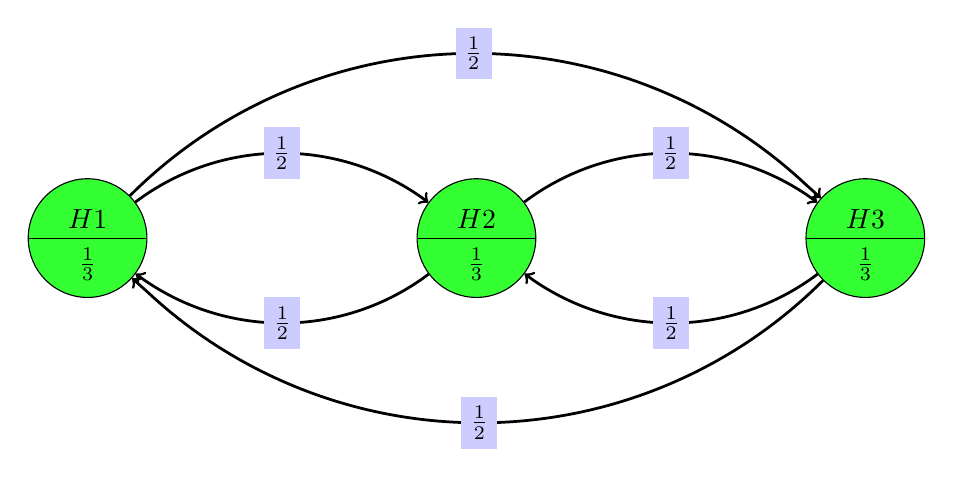
\begin{tikzpicture}[scale=0.7]

\node (H1) at (135.714285714286bp,-235.714285714286bp)[draw,circle split,fill=green!80] {$H1$ \nodepart{lower} $\frac{1}{3}$};
\node (H2) at (335.714285714286bp,-235.714285714286bp)[draw,circle split,fill=green!80] {$H2$ \nodepart{lower} $\frac{1}{3}$};
\node (H3) at (535.714285714286bp,-235.714285714286bp)[draw,circle split,fill=green!80] {$H3$ \nodepart{lower} $\frac{1}{3}$};
\draw [->,line width=1pt] (H1.37) arc(127:90:125bp) node[fill=blue!20] {$\frac{1}{2}$} arc(90:55:125bp) to (H2);
\draw [->,line width=1pt] (H1.45) arc(135:90:250bp) node[fill=blue!20] {$\frac{1}{2}$} arc(90:47:250bp) to (H3);
\draw [->,line width=1pt] (H2.217) arc(307:270:125bp) node[fill=blue!20] {$\frac{1}{2}$} arc(270:235:125bp) to (H1);
\draw [->,line width=1pt] (H2.37) arc(127:90:125bp) node[fill=blue!20] {$\frac{1}{2}$} arc(90:55:125bp) to (H3);
\draw [->,line width=1pt] (H3.225) arc(315:270:250bp) node[fill=blue!20] {$\frac{1}{2}$} arc(270:227:250bp) to (H1);
\draw [->,line width=1pt] (H3.217) arc(307:270:125bp) node[fill=blue!20] {$\frac{1}{2}$} arc(270:235:125bp) to (H2);
\end{tikzpicture}


  \caption{\label{fig:exampleHolm} Graph representing the
    Bonferroni-Holm-Procedure for three hypotheses.}
\end{figure}

A null hypothesis can be rejected, when the p-value is less than the
alpha level of the corresponding node.  In this case the graph will be
updated and the alpha level of this node is passed according to the
edge weights.

\begin{Example}
  We give an example for the Bonferroni-Holm-Procedure.
  %that willbe used repeatedly throughout this manual. 
  Of course this 
  package is made for more advanced tests (you find a selection in 
  appendix \ref{sec:exampleGraphs} with applied examples in section \ref{sec:caseStudies}),
  but since most readers are already familiar with this procedure,
  for a first introduction of gMCP, we stick to this simple example.  
  
  Let $p_1=0.01$, $p_2=0.07$ and $p_3=0.02$ be three p-values and
  $\alpha=0.05$.  In the first step $H_1$ can be rejected since
  $p_1<\alpha/3$.  The updated graph can be seen in figure
  \ref{fig:exampleHolmP} and now also $H_3$ can be rejected since
  $p_1<\alpha/2$.  Again the graph is updated, but $H_2$
  can not be rejected.
\end{Example}

\begin{figure}[ht]
  \centering
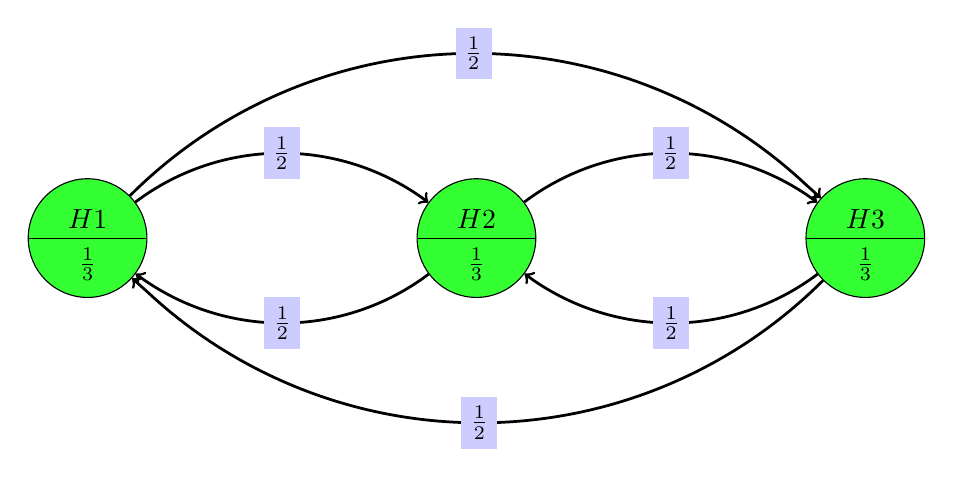
\begin{tikzpicture}[scale=0.7]

\node (H1) at (135.714285714286bp,-235.714285714286bp)[draw,circle split,minimum size=1.2cm, fill=green!80] {$H1$ \nodepart{lower} $\frac{1}{3}$};
\node (H2) at (335.714285714286bp,-235.714285714286bp)[draw,circle split,minimum size=1.2cm, fill=green!80] {$H2$ \nodepart{lower} $\frac{1}{3}$};
\node (H3) at (535.714285714286bp,-235.714285714286bp)[draw,circle split,minimum size=1.2cm, fill=green!80] {$H3$ \nodepart{lower} $\frac{1}{3}$};
\draw [->,line width=1pt] (H1.37) arc(127:90:125bp) node[fill=blue!20] {$\frac{1}{2}$} arc(90:55:125bp) to (H2);
\draw [->,line width=1pt] (H1.45) arc(135:90:250bp) node[fill=blue!20] {$\frac{1}{2}$} arc(90:47:250bp) to (H3);
\draw [->,line width=1pt] (H2.217) arc(307:270:125bp) node[fill=blue!20] {$\frac{1}{2}$} arc(270:235:125bp) to (H1);
\draw [->,line width=1pt] (H2.37) arc(127:90:125bp) node[fill=blue!20] {$\frac{1}{2}$} arc(90:55:125bp) to (H3);
\draw [->,line width=1pt] (H3.225) arc(315:270:250bp) node[fill=blue!20] {$\frac{1}{2}$} arc(270:227:250bp) to (H1);
\draw [->,line width=1pt] (H3.217) arc(307:270:125bp) node[fill=blue!20] {$\frac{1}{2}$} arc(270:235:125bp) to (H2);
\end{tikzpicture}
\\$\downarrow$ reject $H_1$\\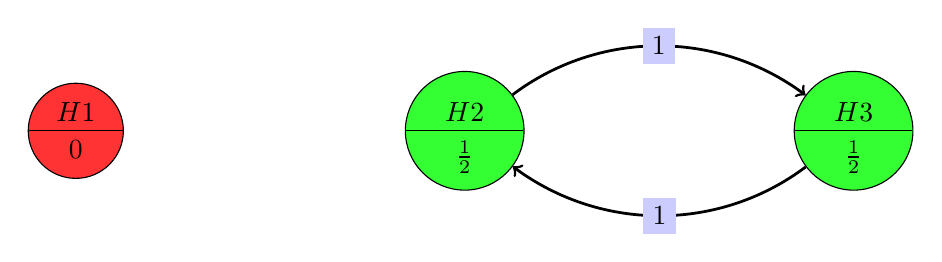
\begin{tikzpicture}[scale=0.7]

\node (H1) at (135.714285714286bp,-235.714285714286bp)[draw,circle split,minimum size=1.2cm, fill=red!80] {$H1$ \nodepart{lower} $0$};
\node (H2) at (335.714285714286bp,-235.714285714286bp)[draw,circle split,minimum size=1.2cm, fill=green!80] {$H2$ \nodepart{lower} $\frac{1}{2}$};
\node (H3) at (535.714285714286bp,-235.714285714286bp)[draw,circle split,minimum size=1.2cm, fill=green!80] {$H3$ \nodepart{lower} $\frac{1}{2}$};
\draw [->,line width=1pt] (H2.37) arc(127:90:125bp) node[fill=blue!20] {$1$} arc(90:55:125bp) to (H3);
\draw [->,line width=1pt] (H3.217) arc(307:270:125bp) node[fill=blue!20] {$1$} arc(270:235:125bp) to (H2);
\end{tikzpicture}
\\$\downarrow$ reject $H_3$\\\ \\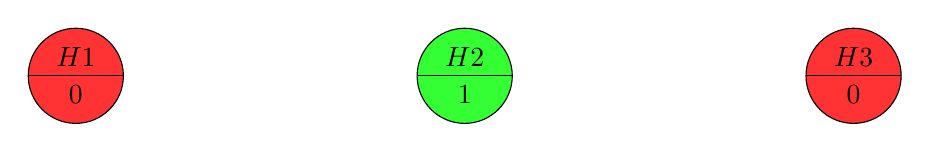
\begin{tikzpicture}[scale=0.7]

\node (H1) at (135.714285714286bp,-235.714285714286bp)[draw,circle split,minimum size=1.2cm, fill=red!80] {$H1$ \nodepart{lower} $0$};
\node (H2) at (335.714285714286bp,-235.714285714286bp)[draw,circle split,minimum size=1.2cm, fill=green!80] {$H2$ \nodepart{lower} $1$};
\node (H3) at (535.714285714286bp,-235.714285714286bp)[draw,circle split,minimum size=1.2cm, fill=red!80] {$H3$ \nodepart{lower} $0$};
\end{tikzpicture}


  \caption{\label{fig:exampleHolmP} Example showing how two
    null hypotheses can be rejected with p-values $p_1=0.01$,
    $p_2=0.07$ and $p_3=0.02$.}
\end{figure}

Let's reproduce this with the \texttt{gMCP} package. We start R and enter:

\begin{knitrout}\footnotesize
\definecolor{shadecolor}{rgb}{0.969, 0.969, 0.969}\color{fgcolor}\begin{kframe}
\begin{alltt}
\hlkwd{library}\hlstd{(gMCP)}
\hlkwd{graphGUI}\hlstd{()}
\end{alltt}
\end{kframe}
\end{knitrout}


The GUI seen in Figure \ref{fig:fullGUI} is shown and we select from the
menu "\emph{Example graphs}" the entry "\emph{Bonferroni-Holm Test}".
We enter the three p-values in the respective fields on the right
side.  By clicking on the button with the green arrow we start the
test procedure and can sequentially reject all three hypotheses.

If we don't want to use the GUI we can also use R:

\begin{knitrout}\footnotesize
\definecolor{shadecolor}{rgb}{0.969, 0.969, 0.969}\color{fgcolor}\begin{kframe}
\begin{alltt}
\hlkwd{library}\hlstd{(gMCP)}
\hlstd{graph} \hlkwb{<-} \hlkwd{BonferroniHolm}\hlstd{(}\hlnum{3}\hlstd{)}
\hlkwd{gMCP}\hlstd{(graph,} \hlkwc{pvalues} \hlstd{=} \hlkwd{c}\hlstd{(}\hlnum{0.01}\hlstd{,} \hlnum{0.07}\hlstd{,} \hlnum{0.02}\hlstd{),} \hlkwc{alpha} \hlstd{=} \hlnum{0.05}\hlstd{)}
\end{alltt}
\begin{verbatim}
## gMCP-Result
## 
## Initial graph:
## A graphMCP graph
## H1 (weight=0.3333)
## H2 (weight=0.3333)
## H3 (weight=0.3333)
## Edges:
## H1  -( 0.5 )->  H2 
## H1  -( 0.5 )->  H3 
## H2  -( 0.5 )->  H1 
## H2  -( 0.5 )->  H3 
## H3  -( 0.5 )->  H1 
## H3  -( 0.5 )->  H2 
## 
## 
## P-values:
##   H1   H2   H3 
## 0.01 0.07 0.02 
## 
## Adjusted p-values:
##   H1   H2   H3 
## 0.03 0.07 0.04 
## 
## Alpha: 0.05 
## 
## Hypothesis rejected:
##    H1    H2    H3 
##  TRUE FALSE  TRUE 
## 
## Final graph after 2 steps:
## A graphMCP graph
## H1 (rejected, weight=0)
## H2 (weight=1)
## H3 (rejected, weight=0)
## No edges.
\end{verbatim}
\end{kframe}
\end{knitrout}


\section{Creating Weighted Graphs}

In the first step a graph that describes the multiple test procedures
must be created.

\begin{figure}[ht]
  \centering   
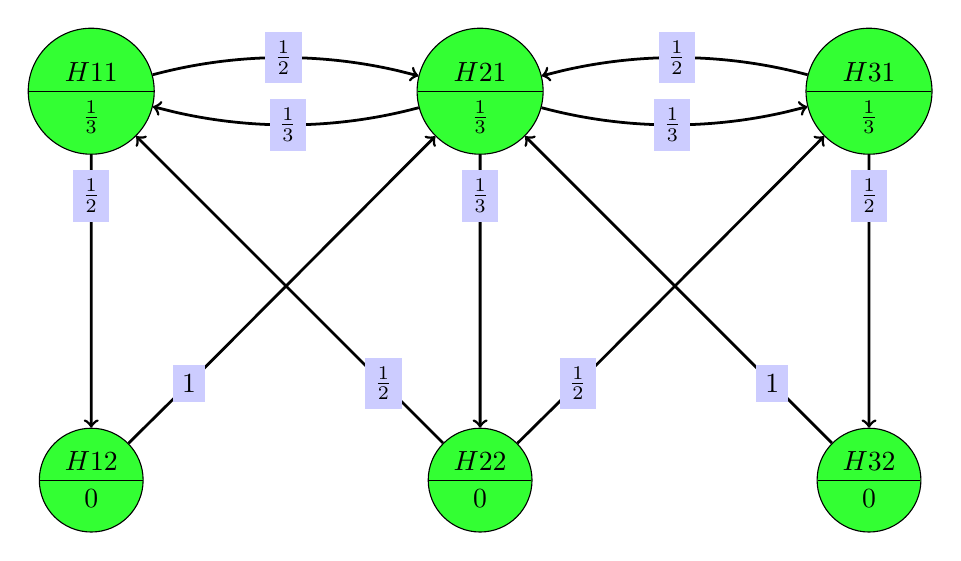
\begin{tikzpicture}[scale=0.7]

\node (H11) at (135.714285714286bp,-135.714285714286bp)[draw,circle split,fill=green!80] {$H11$ \nodepart{lower} $\frac{1}{3}$};
\node (H21) at (335.714285714286bp,-135.714285714286bp)[draw,circle split,fill=green!80] {$H21$ \nodepart{lower} $\frac{1}{3}$};
\node (H31) at (535.714285714286bp,-135.714285714286bp)[draw,circle split,fill=green!80] {$H31$ \nodepart{lower} $\frac{1}{3}$};
\node (H12) at (135.714285714286bp,-335.714285714286bp)[draw,circle split,fill=green!80] {$H12$ \nodepart{lower} $0$};
\node (H22) at (335.714285714286bp,-335.714285714286bp)[draw,circle split,fill=green!80] {$H22$ \nodepart{lower} $0$};
\node (H32) at (535.714285714286bp,-335.714285714286bp)[draw,circle split,fill=green!80] {$H32$ \nodepart{lower} $0$};
\draw [->,line width=1pt] (H11.15) arc(105:90:260bp) node[fill=blue!20] {$\frac{1}{2}$} arc(90:77:260bp) to (H21);
\draw [->,line width=1pt] (H11) to[auto] node[near start,above,fill=blue!20] {$\frac{1}{2}$} (H12);
\draw [->,line width=1pt] (H21.195) arc(285:270:260bp) node[fill=blue!20] {$\frac{1}{3}$} arc(270:257:260bp) to (H11);
\draw [->,line width=1pt] (H21.345) arc(255:270:260bp) node[fill=blue!20] {$\frac{1}{3}$} arc(270:283:260bp) to (H31);
\draw [->,line width=1pt] (H21) to[auto] node[near start,above,fill=blue!20] {$\frac{1}{3}$} (H22);
\draw [->,line width=1pt] (H31.165) arc(75:90:260bp) node[fill=blue!20] {$\frac{1}{2}$} arc(90:103:260bp) to (H21);
\draw [->,line width=1pt] (H31) to[auto] node[near start,above,fill=blue!20] {$\frac{1}{2}$} (H32);
\draw [->,line width=1pt] (H12) to (186bp, -286bp) node[fill=blue!20] {$1$} to (H21);
\draw [->,line width=1pt] (H22) to (286bp, -286bp) node[fill=blue!20] {$\frac{1}{2}$} to (H11);
\draw [->,line width=1pt] (H22) to (386bp, -286bp) node[fill=blue!20] {$\frac{1}{2}$} to (H31);
\draw [->,line width=1pt] (H32) to (486bp, -286bp) node[fill=blue!20] {$1$} to (H21);
\end{tikzpicture}


  \caption{\label{fig:exampleGraphBretz} Example graph from \cite{bretz2011test} that we will create in this vignette.}
\end{figure}

\subsection{Using R}

The most convenient way to create a graph in R is to use the functions
\texttt{matrix2graph}\index{matrix2graph} and
\texttt{setWeights}\index{setWeights}.  As an example we create the
graph from \cite{bretz2011test} that you can see in
figure \ref{fig:exampleGraphBretz}.

\begin{knitrout}\footnotesize
\definecolor{shadecolor}{rgb}{0.969, 0.969, 0.969}\color{fgcolor}\begin{kframe}
\begin{alltt}
\hlstd{m} \hlkwb{<-} \hlkwd{rbind}\hlstd{(}\hlkwc{H11}\hlstd{=}\hlkwd{c}\hlstd{(}\hlnum{0}\hlstd{,}   \hlnum{0.5}\hlstd{,} \hlnum{0}\hlstd{,}   \hlnum{0.5}\hlstd{,} \hlnum{0}\hlstd{,}   \hlnum{0}  \hlstd{),}
           \hlkwc{H21}\hlstd{=}\hlkwd{c}\hlstd{(}\hlnum{1}\hlopt{/}\hlnum{3}\hlstd{,} \hlnum{0}\hlstd{,}   \hlnum{1}\hlopt{/}\hlnum{3}\hlstd{,} \hlnum{0}\hlstd{,}   \hlnum{1}\hlopt{/}\hlnum{3}\hlstd{,} \hlnum{0}  \hlstd{),}
           \hlkwc{H31}\hlstd{=}\hlkwd{c}\hlstd{(}\hlnum{0}\hlstd{,}   \hlnum{0.5}\hlstd{,} \hlnum{0}\hlstd{,}   \hlnum{0}\hlstd{,}   \hlnum{0}\hlstd{,}   \hlnum{0.5}\hlstd{),}
           \hlkwc{H12}\hlstd{=}\hlkwd{c}\hlstd{(}\hlnum{0}\hlstd{,}   \hlnum{1}\hlstd{,}   \hlnum{0}\hlstd{,}   \hlnum{0}\hlstd{,}   \hlnum{0}\hlstd{,}   \hlnum{0}  \hlstd{),}
           \hlkwc{H22}\hlstd{=}\hlkwd{c}\hlstd{(}\hlnum{0.5}\hlstd{,} \hlnum{0}\hlstd{,}   \hlnum{0.5}\hlstd{,} \hlnum{0}\hlstd{,}   \hlnum{0}\hlstd{,}   \hlnum{0}  \hlstd{),}
           \hlkwc{H32}\hlstd{=}\hlkwd{c}\hlstd{(}\hlnum{0}\hlstd{,}   \hlnum{1}\hlstd{,}   \hlnum{0}\hlstd{,}   \hlnum{0}\hlstd{,}   \hlnum{0}\hlstd{,}   \hlnum{0}  \hlstd{))}

\hlstd{graph} \hlkwb{<-} \hlkwd{matrix2graph}\hlstd{(m)}
\hlstd{graph} \hlkwb{<-} \hlkwd{setWeights}\hlstd{(graph,} \hlkwd{c}\hlstd{(}\hlnum{1}\hlopt{/}\hlnum{3}\hlstd{,} \hlnum{1}\hlopt{/}\hlnum{3}\hlstd{,} \hlnum{1}\hlopt{/}\hlnum{3}\hlstd{,} \hlnum{0}\hlstd{,} \hlnum{0}\hlstd{,} \hlnum{0}\hlstd{))}
\end{alltt}
\end{kframe}
\end{knitrout}


For accessing the weights and transition matrix of an existing graph
the functions \texttt{getWeights} and \texttt{getMatrix} are provided.

Let's print the newly created graph:

\begin{knitrout}\footnotesize
\definecolor{shadecolor}{rgb}{0.969, 0.969, 0.969}\color{fgcolor}\begin{kframe}
\begin{alltt}
\hlkwd{print}\hlstd{(graph)}
\end{alltt}
\begin{verbatim}
## A graphMCP graph
## H11 (weight=0.3333)
## H21 (weight=0.3333)
## H31 (weight=0.3333)
## H12 (weight=0)
## H22 (weight=0)
## H32 (weight=0)
## Edges:
## H11  -( 0.5 )->  H21 
## H11  -( 0.5 )->  H12 
## H21  -( 0.333333333333333 )->  H11 
## H21  -( 0.333333333333333 )->  H31 
## H21  -( 0.333333333333333 )->  H22 
## H31  -( 0.5 )->  H21 
## H31  -( 0.5 )->  H32 
## H12  -( 1 )->  H21 
## H22  -( 0.5 )->  H11 
## H22  -( 0.5 )->  H31 
## H32  -( 1 )->  H21
\end{verbatim}
\end{kframe}
\end{knitrout}


Since we also want to visualize the graph, we set two node attributes
\texttt{X} and \texttt{Y} (for further information see the manual
pages of method \texttt{nodeAttr}).

\begin{knitrout}\footnotesize
\definecolor{shadecolor}{rgb}{0.969, 0.969, 0.969}\color{fgcolor}\begin{kframe}
\begin{alltt}
\hlstd{graph}\hlopt{@}\hlkwc{nodeAttr}\hlopt{$}\hlstd{X} \hlkwb{<-} \hlkwd{c}\hlstd{(}\hlkwc{H11} \hlstd{=} \hlnum{100}\hlstd{,} \hlkwc{H21} \hlstd{=} \hlnum{300}\hlstd{,} \hlkwc{H31} \hlstd{=} \hlnum{500}\hlstd{,} \hlkwc{H12} \hlstd{=} \hlnum{100}\hlstd{,} \hlkwc{H22} \hlstd{=} \hlnum{300}\hlstd{,} \hlkwc{H32} \hlstd{=} \hlnum{500}\hlstd{)}
\hlstd{graph}\hlopt{@}\hlkwc{nodeAttr}\hlopt{$}\hlstd{Y} \hlkwb{<-} \hlkwd{c}\hlstd{(}\hlkwc{H11} \hlstd{=} \hlnum{100}\hlstd{,} \hlkwc{H21} \hlstd{=} \hlnum{100}\hlstd{,} \hlkwc{H31} \hlstd{=} \hlnum{100}\hlstd{,} \hlkwc{H12} \hlstd{=} \hlnum{300}\hlstd{,} \hlkwc{H22} \hlstd{=} \hlnum{300}\hlstd{,} \hlkwc{H32} \hlstd{=} \hlnum{300}\hlstd{)}
\end{alltt}
\end{kframe}
\end{knitrout}


For placement of the nodes in a matrix pattern, the function
\texttt{placeNodes} is helpful. The following code does the same as
the two lines of R code above.

\begin{knitrout}\footnotesize
\definecolor{shadecolor}{rgb}{0.969, 0.969, 0.969}\color{fgcolor}\begin{kframe}
\begin{alltt}
\hlstd{graph} \hlkwb{<-} \hlkwd{placeNodes}\hlstd{(graph,} \hlkwc{nrow} \hlstd{=} \hlnum{2}\hlstd{)}
\end{alltt}
\end{kframe}
\end{knitrout}


Coordinates are interpretated as pixels in the GUI and big points in
{\LaTeX} (72 bp = 1 inch).\index{coordinates}

Let's take a look at the graph in {\LaTeX} rendered with package TikZ from 
\cite{TikZ}\index{TikZ} (figure
\ref{fig:exampleGraphBretz} shows the compiled result):

%\lstset{language=[LaTeX]TeX}
%\begin{lstlisting}
\begin{knitrout}\footnotesize
\definecolor{shadecolor}{rgb}{0.969, 0.969, 0.969}\color{fgcolor}\begin{kframe}
\begin{alltt}
\hlkwd{cat}\hlstd{(}\hlkwd{graph2latex}\hlstd{(graph))}
\end{alltt}
\begin{verbatim}
## \begin{tikzpicture}
## 
## \node (H11) at (125bp,-125bp)[draw,circle split,fill=green!80] {$H11$ \nodepart{lower} $\frac{1}{3}$};
## \node (H21) at (325bp,-125bp)[draw,circle split,fill=green!80] {$H21$ \nodepart{lower} $\frac{1}{3}$};
## \node (H31) at (525bp,-125bp)[draw,circle split,fill=green!80] {$H31$ \nodepart{lower} $\frac{1}{3}$};
## \node (H12) at (125bp,-325bp)[draw,circle split,fill=green!80] {$H12$ \nodepart{lower} $0$};
## \node (H22) at (325bp,-325bp)[draw,circle split,fill=green!80] {$H22$ \nodepart{lower} $0$};
## \node (H32) at (525bp,-325bp)[draw,circle split,fill=green!80] {$H32$ \nodepart{lower} $0$};
## \draw [->,line width=1pt] (H11) to[bend left=15] node[near start,above,fill=blue!20] {$\frac{1}{2}$} (H21);
## \draw [->,line width=1pt] (H11) to[auto] node[near start,above,fill=blue!20] {$\frac{1}{2}$} (H12);
## \draw [->,line width=1pt] (H21) to[bend left=15] node[near start,above,fill=blue!20] {$\frac{1}{3}$} (H11);
## \draw [->,line width=1pt] (H21) to[bend left=15] node[near start,above,fill=blue!20] {$\frac{1}{3}$} (H31);
## \draw [->,line width=1pt] (H21) to[auto] node[near start,above,fill=blue!20] {$\frac{1}{3}$} (H22);
## \draw [->,line width=1pt] (H31) to[bend left=15] node[near start,above,fill=blue!20] {$\frac{1}{2}$} (H21);
## \draw [->,line width=1pt] (H31) to[auto] node[near start,above,fill=blue!20] {$\frac{1}{2}$} (H32);
## \draw [->,line width=1pt] (H12) to[auto] node[near start,above,fill=blue!20] {$1$} (H21);
## \draw [->,line width=1pt] (H22) to[auto] node[near start,above,fill=blue!20] {$\frac{1}{2}$} (H11);
## \draw [->,line width=1pt] (H22) to[auto] node[near start,above,fill=blue!20] {$\frac{1}{2}$} (H31);
## \draw [->,line width=1pt] (H32) to[auto] node[near start,above,fill=blue!20] {$1$} (H21);
## \end{tikzpicture}
\end{verbatim}
\end{kframe}
\end{knitrout}

%\end{lstlisting}

We can even change the position of the edge labels for further fine
tuning of the graphical representation.  With the following command we
place the label for the edge from \texttt{H1} to \texttt{H2} at
position (200, 80):

\begin{knitrout}\footnotesize
\definecolor{shadecolor}{rgb}{0.969, 0.969, 0.969}\color{fgcolor}\begin{kframe}
\begin{alltt}
\hlkwd{edgeAttr}\hlstd{(graph,} \hlstr{"H11"}\hlstd{,} \hlstr{"H21"}\hlstd{,} \hlstr{"labelX"}\hlstd{)} \hlkwb{<-} \hlnum{200}
\hlkwd{edgeAttr}\hlstd{(graph,} \hlstr{"H11"}\hlstd{,} \hlstr{"H21"}\hlstd{,} \hlstr{"labelY"}\hlstd{)} \hlkwb{<-} \hlnum{80}
\end{alltt}
\end{kframe}
\end{knitrout}


\subsection{Using the GUI}

The creation of \texttt{graphMCP} objects as seen in the last section 
with basic R commands is very straight forward,
but still takes some time and typos may occur.  More convenient for
the most users is the use of the graphical user interface for
creating and editing MCP graphs that the \texttt{gMCP} package
includes.

It is called by the command \texttt{graphGUI()} and takes as optional
argument a variable name, given as a character string, of the graph to
edit.
% or under which a newly created \texttt{graphMCP} object will be
% available from the R command line.

\begin{knitrout}\footnotesize
\definecolor{shadecolor}{rgb}{0.969, 0.969, 0.969}\color{fgcolor}\begin{kframe}
\begin{alltt}
\hlkwd{graphGUI}\hlstd{(}\hlstr{"graph"}\hlstd{)}
\end{alltt}
\end{kframe}
\end{knitrout}


\begin{figure}[ht]
  \centering    
  \includegraphics[width=0.95\textwidth]{pictures/FullFeaturedGUI.png}      
  \caption{\label{fig:fullGUI} The graphical user interface allows testing, calculation of confidence intervals and adjusted p-values.}
\end{figure}

Let's take a look at the icon panel:

\includegraphics[width=0.5cm]{pictures/vertex.png} This button lets
you add a new node to the graph.  After pressing the button click
somewhere on the graph panel and a new node will appear at this place.

\includegraphics[width=0.5cm]{pictures/edge.png} This button lets you
add a new edge between two nodes.  After pressing the button click on
the node the edge should start and after that on the node the edge
should end.

\includegraphics[width=0.5cm]{pictures/zoom_in.png}
\includegraphics[width=0.5cm]{pictures/zoom_out.png} For really big
graphs the ability to zoom in and out is usefull.

\includegraphics[width=0.5cm]{pictures/StartTesting.png}
\includegraphics[width=0.5cm]{pictures/Reset.png} Starts the testing
procedure / goes back to the graph modification.

\includegraphics[width=0.5cm]{pictures/adjPval.png} Calculates the
adjusted p-values.

\includegraphics[width=0.5cm]{pictures/confint2.png} Calculates
simultaneous confidence intervals.

With drag and drop you can move nodes and also adjust edges. Double
clicking the nodes or edges will open a property dialog that can also
be accessed via the right-click context menu. These dialogs and
context menus also give you the option to delete the selected
node/edge.

As seen in figure \ref{fig:guircode} the GUI will show you R code to
reproduce results.

\begin{figure}[ht]
  \centering   
  \includegraphics[width=0.7\textwidth]{pictures/GeneratedRCode.png}      
  \caption{\label{fig:guircode} R Code generated and shown by the GUI to reproduce the results.}
\end{figure}

\section{The sequentially rejective MTP}

For a full description of the sequentially rejective multiple testing
procedure take a look at \cite{bretzEtAl2009graphical}. 

\subsection{Using R}

You can either specify each rejection step yourself or simply use the 
method \texttt{gMCP}:

\begin{knitrout}\footnotesize
\definecolor{shadecolor}{rgb}{0.969, 0.969, 0.969}\color{fgcolor}\begin{kframe}
\begin{alltt}
\hlstd{graph} \hlkwb{<-} \hlkwd{BretzEtAl2011}\hlstd{()}

\hlcom{# We can reject a single node:}
\hlkwd{print}\hlstd{(}\hlkwd{rejectNode}\hlstd{(graph,} \hlstr{"H11"}\hlstd{))}
\end{alltt}
\begin{verbatim}
## A graphMCP graph
## H11 (rejected, weight=0)
## H21 (weight=0.5)
## H31 (weight=0.3333)
## H12 (weight=0.1667)
## H22 (weight=0)
## H32 (weight=0)
## Edges:
## H21  -( 0.4 )->  H31 
## H21  -( 0.2 )->  H12 
## H21  -( 0.4 )->  H22 
## H31  -( 0.5 )->  H21 
## H31  -( 0.5 )->  H32 
## H12  -( 1 )->  H21 
## H22  -( 0.25 )->  H21 
## H22  -( 0.5 )->  H31 
## H22  -( 0.25 )->  H12 
## H32  -( 1 )->  H21
\end{verbatim}
\begin{alltt}
\hlcom{# Or given a vector of pvalues let the function gMCP do all the work:  }
\hlstd{pvalues} \hlkwb{<-} \hlkwd{c}\hlstd{(}\hlnum{0.1}\hlstd{,} \hlnum{0.008}\hlstd{,} \hlnum{0.005}\hlstd{,} \hlnum{0.15}\hlstd{,} \hlnum{0.04}\hlstd{,} \hlnum{0.006}\hlstd{)}
\hlstd{result} \hlkwb{<-} \hlkwd{gMCP}\hlstd{(graph, pvalues)}
\hlkwd{print}\hlstd{(result)}
\end{alltt}
\begin{verbatim}
## gMCP-Result
## 
## Initial graph:
## A graphMCP graph
## H11 (weight=0.3333)
## H21 (weight=0.3333)
## H31 (weight=0.3333)
## H12 (weight=0)
## H22 (weight=0)
## H32 (weight=0)
## Edges:
## H11  -( 0.5 )->  H21 
## H11  -( 0.5 )->  H12 
## H21  -( 0.333333333333333 )->  H11 
## H21  -( 0.333333333333333 )->  H31 
## H21  -( 0.333333333333333 )->  H22 
## H31  -( 0.5 )->  H21 
## H31  -( 0.5 )->  H32 
## H12  -( 1 )->  H21 
## H22  -( 0.5 )->  H11 
## H22  -( 0.5 )->  H31 
## H32  -( 1 )->  H21 
## 
## 
## P-values:
##   H11   H21   H31   H12   H22   H32 
## 0.100 0.008 0.005 0.150 0.040 0.006 
## 
## Adjusted p-values:
##    H11    H21    H31    H12    H22    H32 
## 0.1200 0.0160 0.0150 0.1500 0.1200 0.0225 
## 
## Alpha: 0.05 
## 
## Hypothesis rejected:
##   H11   H21   H31   H12   H22   H32 
## FALSE  TRUE  TRUE FALSE FALSE  TRUE 
## 
## Final graph after 3 steps:
## A graphMCP graph
## H11 (weight=0.6667)
## H21 (rejected, weight=0)
## H31 (rejected, weight=0)
## H12 (weight=0)
## H22 (weight=0.3333)
## H32 (rejected, weight=0)
## Edges:
## H11  -( 0.666666666666667 )->  H12 
## H11  -( 0.333333333333333 )->  H22 
## H12  -( 0.5 )->  H11 
## H12  -( 0.5 )->  H22 
## H22  -( 1 )->  H11
\end{verbatim}
\end{kframe}
\end{knitrout}


We can create a TikZ graphic from the last graph with 
\texttt{graph2latex(result@graphs[[4]])} that is shown in figure \ref{fig:finalstate}.

\begin{figure}[ht]
  \centering   
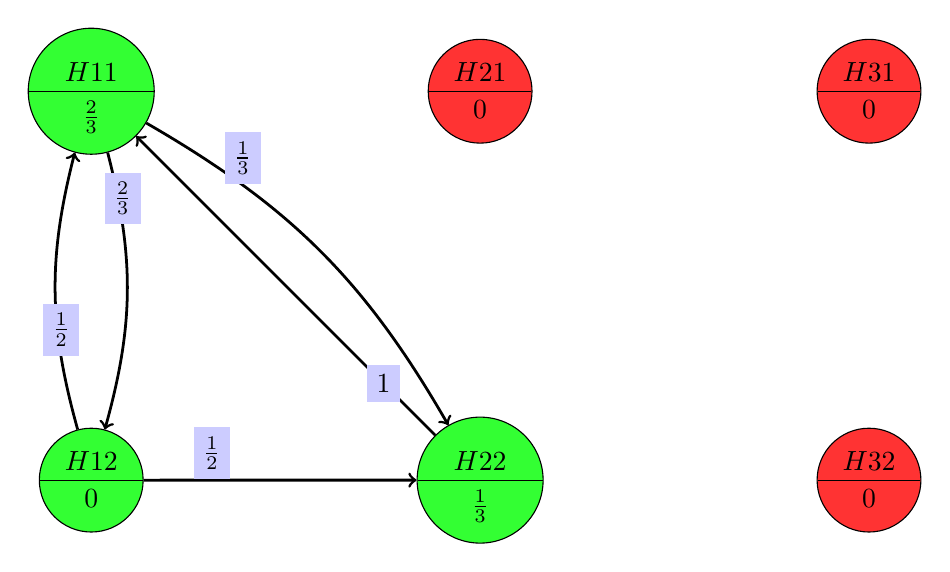
\begin{tikzpicture}[scale=0.7]

\node (H11) at (135.714285714286bp,-135.714285714286bp)[draw,circle split,fill=green!80] {$H11$ \nodepart{lower} $\frac{2}{3}$};
\node (H21) at (335.714285714286bp,-135.714285714286bp)[draw,circle split,fill=red!80] {$H21$ \nodepart{lower} $0$};
\node (H31) at (535.714285714286bp,-135.714285714286bp)[draw,circle split,fill=red!80] {$H31$ \nodepart{lower} $0$};
\node (H12) at (135.714285714286bp,-335.714285714286bp)[draw,circle split,fill=green!80] {$H12$ \nodepart{lower} $0$};
\node (H22) at (335.714285714286bp,-335.714285714286bp)[draw,circle split,fill=green!80] {$H22$ \nodepart{lower} $\frac{1}{3}$};
\node (H32) at (535.714285714286bp,-335.714285714286bp)[draw,circle split,fill=red!80] {$H32$ \nodepart{lower} $0$};
\draw [->,line width=1pt] (H11) to[bend left=15] node[near start,above,fill=blue!20] {$\frac{2}{3}$} (H12);
\draw [->,line width=1pt] (H11) to[bend left=15] node[near start,above,fill=blue!20] {$\frac{1}{3}$} (H22);
\draw [->,line width=1pt] (H12) to[bend left=15] node[near start,above,fill=blue!20] {$\frac{1}{2}$} (H11);
\draw [->,line width=1pt] (H12) to[auto] node[near start,above,fill=blue!20] {$\frac{1}{2}$} (H22);
\draw [->,line width=1pt] (H22) to (286bp, -286bp) node[fill=blue!20] {$1$} to (H11);
\end{tikzpicture}


  \caption{\label{fig:finalstate}Final graph from the test procedure after rejection of $H_{21}$, $H_{31}$ and $H_{32}$.}
\end{figure}

The command \texttt{gMCPReport}\index{report generation} generates a
full report of the testing procedure:

\begin{knitrout}\footnotesize
\definecolor{shadecolor}{rgb}{0.969, 0.969, 0.969}\color{fgcolor}\begin{kframe}
\begin{alltt}
\hlkwd{gMCPReport}\hlstd{(result,} \hlstr{"Report.tex"}\hlstd{)}
\end{alltt}
\end{kframe}
\end{knitrout}


\subsubsection{Adjusted p-values and simultaneous confidence intervals}\index{adjusted p-values}\index{simultaneous confidence intervals}

Also adjusted p-values and simultaneous confidence intervals can be computed.




Let's assume the tests for hypotheses $H1:\;\theta_1\leq0$,
$H2:\;\theta_2\leq0$ and $H3:\;\theta_3\leq0$ are three t-tests with degree
of freedom 9.  The estimates are
$\hat\theta_1=0.981$,
$\hat\theta_2=1.089$ and
$\hat\theta_3=0.8706$, the sample standard deviations
$s_1=0.876$,
$s_2=1.291$ and
$s_3=0.8571$ the t-statistics
$3.541$, $2.666$ and
$3.212$ and the corresponding p-values $0.0063$, 
$0.02577$ and
$0.01062$.  We want to adjust for multiple testing
by using the Bonferroni-Holm-Procedure with $\alpha=0.025$.

\begin{knitrout}\footnotesize
\definecolor{shadecolor}{rgb}{0.969, 0.969, 0.969}\color{fgcolor}\begin{kframe}
\begin{alltt}
\hlcom{# Estimates:}
\hlstd{est} \hlkwb{<-} \hlkwd{c}\hlstd{(}\hlstr{"H1"}\hlstd{=}\hlnum{0.860382}\hlstd{,} \hlstr{"H2"}\hlstd{=}\hlnum{0.9161474}\hlstd{,} \hlstr{"H3"}\hlstd{=}\hlnum{0.9732953}\hlstd{)}
\hlcom{# Sample standard deviations:}
\hlstd{ssd} \hlkwb{<-} \hlkwd{c}\hlstd{(}\hlstr{"H1"}\hlstd{=}\hlnum{0.8759528}\hlstd{,} \hlstr{"H2"}\hlstd{=}\hlnum{1.291310}\hlstd{,} \hlstr{"H3"}\hlstd{=}\hlnum{0.8570892}\hlstd{)}

\hlstd{pval} \hlkwb{<-} \hlkwd{c}\hlstd{(}\hlnum{0.01260}\hlstd{,} \hlnum{0.05154}\hlstd{,} \hlnum{0.02124}\hlstd{)}\hlopt{/}\hlnum{2}

\hlkwd{simConfint}\hlstd{(}\hlkwd{BonferroniHolm}\hlstd{(}\hlnum{3}\hlstd{),} \hlkwc{pvalues}\hlstd{=pval,}
                \hlkwc{confint}\hlstd{=}\hlkwa{function}\hlstd{(}\hlkwc{node}\hlstd{,} \hlkwc{alpha}\hlstd{) \{}
                        \hlkwd{c}\hlstd{(est[node]}\hlopt{-}\hlkwd{qt}\hlstd{(}\hlnum{1}\hlopt{-}\hlstd{alpha,}\hlkwc{df}\hlstd{=}\hlnum{9}\hlstd{)}\hlopt{*}\hlstd{ssd[node]}\hlopt{/}\hlkwd{sqrt}\hlstd{(}\hlnum{10}\hlstd{),} \hlnum{Inf}\hlstd{)}
                \hlstd{\},} \hlkwc{estimates}\hlstd{=est,} \hlkwc{alpha}\hlstd{=}\hlnum{0.025}\hlstd{,} \hlkwc{mu}\hlstd{=}\hlnum{0}\hlstd{,} \hlkwc{alternative}\hlstd{=}\hlstr{"greater"}\hlstd{)}
\end{alltt}
\begin{verbatim}
##    lower bound estimate upper bound
## H1      0.0000   0.8604         Inf
## H2     -0.0076   0.9161         Inf
## H3      0.0000   0.9733         Inf
\end{verbatim}
\begin{alltt}
\hlcom{# Note that the sample standard deviations in the following call}
\hlcom{# will be calculated from the pvalues and estimates.}
\hlkwd{simConfint}\hlstd{(}\hlkwd{BonferroniHolm}\hlstd{(}\hlnum{3}\hlstd{),} \hlkwc{pvalues}\hlstd{=pval,}
                \hlkwc{confint}\hlstd{=}\hlstr{"t"}\hlstd{,} \hlkwc{df}\hlstd{=}\hlnum{9}\hlstd{,} \hlkwc{estimates}\hlstd{=est,} \hlkwc{alpha}\hlstd{=}\hlnum{0.025}\hlstd{,} \hlkwc{alternative}\hlstd{=}\hlstr{"greater"}\hlstd{)}
\end{alltt}
\begin{verbatim}
##      lower bound estimate upper bound
## [1,]    0.000000   0.8604         Inf
## [2,]   -0.007581   0.9161         Inf
## [3,]    0.000000   0.9733         Inf
\end{verbatim}
\end{kframe}
\end{knitrout}


\subsection{Using the GUI}

\begin{figure}[ht]
  \centering    
  \includegraphics[width=0.7\textwidth]{pictures/CIDialog.png}      
  \caption{\label{fig:CIDialog} For normal and t-distributions simultaneous CI can be calculated by the GUI.}
\end{figure}


Use the following two buttons:
\includegraphics[width=1cm]{pictures/adjPval_b.png}
\includegraphics[width=1cm]{pictures/confint2_b.png}

See \cite{Bretz11}.

\section{Weighted parametric and Simes
tests}\index{Simes-Procedure}\index{parametric test} 

\begin{figure}[ht]
  \centering    
  \includegraphics[width=0.7\textwidth]{pictures/correlated.png}      
  \caption{\label{fig:correlated} You can also specify a correlation between the tests.}
\end{figure}

In the lower right panel with p-values, it is also possible to specify a known
correlation between the original test statistics (see figure
\ref{fig:correlated}). Either you can perform a Simes test or a weighted parametric
tests as described in \cite{Bretz11}. For the later it is assumed that
under the global null hypothesis $(\Phi^{-1}(1-p_1),\ldots,\Phi^{-1}(1-p_m))$ 
follow a multivariate normal distribution with correlation matrix $\Sigma$ where
$\Phi^{-1}$ denotes the inverse of the standard normal
distribution function. For example, this is the case if $p_1,\ldots,
  p_m$ are the raw p-values from one-sided $z$-tests for each of the
elementary hypotheses where the correlation between z-test statistics
is generated by an overlap in the observations (e.g. comparison with a
common control, group-sequential analyses etc.). An application of the
transformation $\Phi^{-1}(1-p_i)$ to raw p-values from a two-sided
test will not in general lead to a multivariate normal
distribution.

For further information please take a look at the vignette
"\href{http://cran.r-project.org/web/packages/gMCP/vignettes/parametric.pdf}{Weighted
parametric tests defined by graphs}".

\subsection{Correlation matrix creation}\index{correlation matrix}

The GUI features a dialog for easy creation of correlation matrices (see figure \ref{fig:createCM1}).

\begin{figure}[ht]
  \centering    
  \includegraphics[width=\textwidth]{pictures/createCM3.png}      
  \caption{\label{fig:createCM1} Dialog for specifying a correlation matrix.}
\end{figure}

If the entered matrix is not positive semidefinite, 
i.e.\ negative eigen values exist, a warning is given.

This dialog is perhaps useful on its own and can be opened by 
calling the function \texttt{corMatWizard}.

%\[A \kronecker B\]

%\begin{figure}[ht]
%  \centering    
%  \includegraphics[width=0.7\textwidth]{pictures/createCM1.png}      
%  \caption{\label{fig:createCM2} You can configure many things in the option dialog.}
%\end{figure}

%\begin{figure}[ht]
%  \centering    
%  \includegraphics[width=0.7\textwidth]{pictures/createCM1.png}      
%  \caption{\label{fig:createCM3} You can configure many things in the option dialog.}
%\end{figure}

\section{Epsilon edges}\index{epsilon edges}

%\begin{Def}
  %Convergence in distribution
  %Convergence in probability
  %Almost sure convergence
  %Sure convergence
  %Convergence in the r-th mean
%\end{Def}

The GUI supports epsilon edges. You can enter the weights in R syntax,
e.g.\ \texttt{1-2*\textbackslash epsilon+1/3*\textbackslash epsilon\^{}2} for $1-2\epsilon+\frac{1}{3}\epsilon^2$.

\begin{figure}[ht]
  \centering
  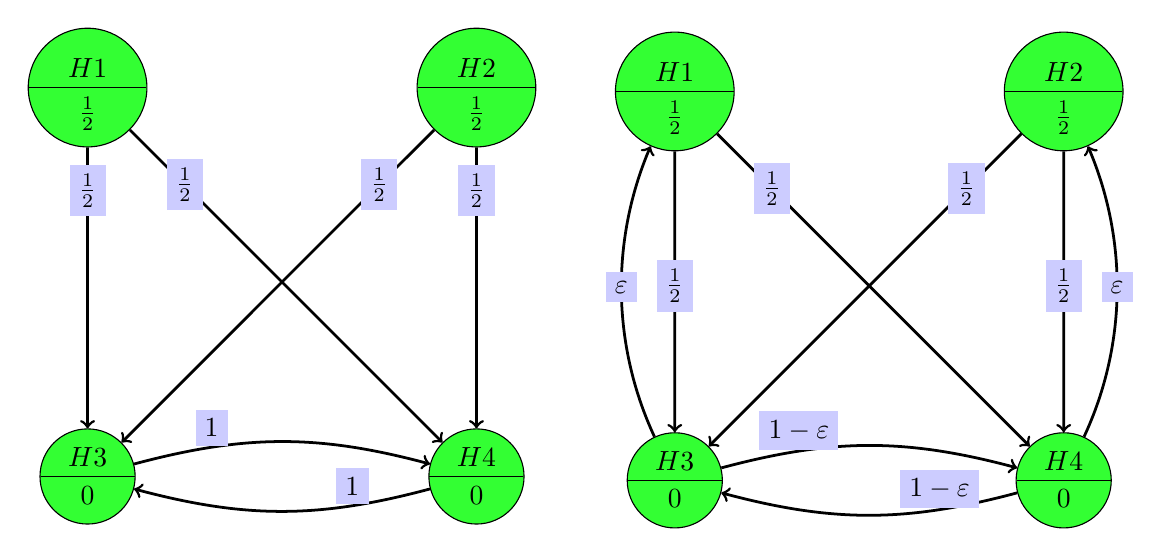
\begin{tikzpicture}[scale=0.7]
% Chunk 19

\node (H1) at (125bp,-125bp)[draw,circle split,minimum size=1.2cm, fill=green!80] {$H1$ \nodepart{lower} $\frac{1}{2}$};
\node (H2) at (325bp,-125bp)[draw,circle split,minimum size=1.2cm, fill=green!80] {$H2$ \nodepart{lower} $\frac{1}{2}$};
\node (H3) at (125bp,-325bp)[draw,circle split,minimum size=1.2cm, fill=green!80] {$H3$ \nodepart{lower} $0$};
\node (H4) at (325bp,-325bp)[draw,circle split,minimum size=1.2cm, fill=green!80] {$H4$ \nodepart{lower} $0$};
\draw [->,line width=1pt] (H1) to[auto] node[near start,above,fill=blue!20] {$\frac{1}{2}$} (H3);
\draw [->,line width=1pt] (H1) to (175bp, -175bp) node[fill=blue!20] {$\frac{1}{2}$} to (H4);
\draw [->,line width=1pt] (H2) to (275bp, -175bp) node[fill=blue!20] {$\frac{1}{2}$} to (H3);
\draw [->,line width=1pt] (H2) to[auto] node[near start,above,fill=blue!20] {$\frac{1}{2}$} (H4);
\draw [->,line width=1pt] (H3) to[bend left=15] node[near start,above,fill=blue!20] {$1$} (H4);
\draw [->,line width=1pt] (H4) to[bend left=15] node[near start,above,fill=blue!20] {$1$} (H3);
\node (H1) at (427bp,-127bp)[draw,circle split,minimum size=1.2cm, fill=green!80] {$H1$ \nodepart{lower} $\frac{1}{2}$};
\node (H2) at (627bp,-127bp)[draw,circle split,minimum size=1.2cm, fill=green!80] {$H2$ \nodepart{lower} $\frac{1}{2}$};
\node (H3) at (427bp,-327bp)[draw,circle split,minimum size=1.2cm, fill=green!80] {$H3$ \nodepart{lower} $0$};
\node (H4) at (627bp,-327bp)[draw,circle split,minimum size=1.2cm, fill=green!80] {$H4$ \nodepart{lower} $0$};
\draw [->,line width=1pt] (H1) to (427bp, -227bp) node[fill=blue!20] {$\frac{1}{2}$} to (H3);
\draw [->,line width=1pt] (H1) to (477bp, -177bp) node[fill=blue!20] {$\frac{1}{2}$} to (H4);
\draw [->,line width=1pt] (H2) to (577bp, -177bp) node[fill=blue!20] {$\frac{1}{2}$} to (H3);
\draw [->,line width=1pt] (H2) to (627bp, -227bp) node[fill=blue!20] {$\frac{1}{2}$} to (H4);
\draw [->,line width=1pt] (H3.115) arc(205:180:182bp) node[fill=blue!20] {$\epsilon$} arc(180:157:182bp) to (H1);
\draw [->,line width=1pt] (H3) to[bend left=15] node[near start,above,fill=blue!20] {$1-\epsilon$} (H4);
\draw [->,line width=1pt] (H4.425) arc(335:360:182bp) node[fill=blue!20] {$\epsilon$} arc(360:383:182bp) to (H2);
\draw [->,line width=1pt] (H4) to[bend left=15] node[near start,above,fill=blue!20] {$1-\epsilon$} (H3);

\end{tikzpicture}
  \caption{\label{fig:gatekeeping}\index{parallel gatekeeping}\index{gatekeeping!parallel}\index{gatekeeping!improved parallel} The Parallel Gatekeeping and the Improved Parallel Gatekeeping Procedure.}
\end{figure}


%Algorithm of Bretz et al. from \cite{bretz2011test} for rejecting a node:

%\[\alpha_l \leftarrow \begin{cases}\alpha_l+a_jg_{jl}&l\in I\\0&\text{otherwise}\end{cases}\]

%\[g_{lk} \leftarrow \begin{cases}\frac{g_{lk}+g_{lj}g_{jk}}{1-g_{lj}g_{jl}}&k,l\in I, l\neq k, g_{lj}g_{jl}<1\\0&\text{otherwise}\end{cases}\]

%We want now investigate what happens if a edge weight $\epsilon>0$ approaches
% $0$.
%In respect to 

%\[\alpha_l \leftarrow \begin{cases}0=\lim\limits_{g_{jl}\rightarrow0}(\alpha_l+a_jg_{jl})&l\in I\\0&\text{otherwise}\end{cases}\]

%The only question is, what happens if and $l\in I, l\neq k, g_{lj}g_{jl}<1$.
%If $g_{lj}g_{jl}==1$ still $g_{lk}<-0$.
 
%\[\lim\limits_{g_{jl}\rightarrow0}\left(\frac{g_{lk}+g_{lj}g_{jk}}{1-g_{lj}g_{jl}}\right)
%=\begin{cases}
%  \frac{g_{lk}+g_{lj}g_{jk}}{1-g_{lj}g_{jl}}&g_{lj}g_{jl}<1\\
%  0&g_{lj}g_{jl}=1\\a\\b\\\end{cases}
%=\]


\begin{knitrout}\footnotesize
\definecolor{shadecolor}{rgb}{0.969, 0.969, 0.969}\color{fgcolor}\begin{kframe}
\begin{alltt}
\hlstd{m} \hlkwb{<-} \hlkwd{rbind}\hlstd{(}\hlkwc{H1}\hlstd{=}\hlkwd{c}\hlstd{(}\hlnum{0}\hlstd{,}           \hlnum{0}\hlstd{,}           \hlnum{0.5}\hlstd{,}           \hlnum{0.5}          \hlstd{),}
           \hlkwc{H2}\hlstd{=}\hlkwd{c}\hlstd{(}\hlnum{0}\hlstd{,}           \hlnum{0}\hlstd{,}           \hlnum{0.5}\hlstd{,}           \hlnum{0.5}          \hlstd{),}
           \hlkwc{H3}\hlstd{=}\hlkwd{c}\hlstd{(}\hlstr{"\textbackslash{}\textbackslash{}epsilon"}\hlstd{,} \hlnum{0}\hlstd{,}           \hlnum{0}\hlstd{,}             \hlstr{"1-\textbackslash{}\textbackslash{}epsilon"}\hlstd{),}
           \hlkwc{H4}\hlstd{=}\hlkwd{c}\hlstd{(}\hlnum{0}\hlstd{,}           \hlstr{"\textbackslash{}\textbackslash{}epsilon"}\hlstd{,} \hlstr{"1-\textbackslash{}\textbackslash{}epsilon"}\hlstd{,} \hlnum{0}            \hlstd{))}

\hlstd{graph} \hlkwb{<-} \hlkwd{matrix2graph}\hlstd{(m)}
\hlcom{#graph <- improvedParallelGatekeeping()}
\hlstd{graph}
\end{alltt}
\begin{verbatim}
## A graphMCP graph
## H1 (weight=0.25)
## H2 (weight=0.25)
## H3 (weight=0.25)
## H4 (weight=0.25)
## Edges:
## H1  -( 0.5 )->  H3 
## H1  -( 0.5 )->  H4 
## H2  -( 0.5 )->  H3 
## H2  -( 0.5 )->  H4 
## H3  -( \epsilon )->  H1 
## H3  -( 1-\epsilon )->  H4 
## H4  -( \epsilon )->  H2 
## H4  -( 1-\epsilon )->  H3
\end{verbatim}
\begin{alltt}
\hlkwd{substituteEps}\hlstd{(graph,} \hlkwc{eps}\hlstd{=}\hlnum{0.001}\hlstd{)}
\end{alltt}
\begin{verbatim}
## A graphMCP graph
## H1 (weight=0.25)
## H2 (weight=0.25)
## H3 (weight=0.25)
## H4 (weight=0.25)
## Edges:
## H1  -( 0.5 )->  H3 
## H1  -( 0.5 )->  H4 
## H2  -( 0.5 )->  H3 
## H2  -( 0.5 )->  H4 
## H3  -( 0.001 )->  H1 
## H3  -( 0.999 )->  H4 
## H4  -( 0.001 )->  H2 
## H4  -( 0.999 )->  H3
\end{verbatim}
\begin{alltt}
\hlkwd{gMCP}\hlstd{(graph,} \hlkwc{pvalues}\hlstd{=}\hlkwd{c}\hlstd{(}\hlnum{0.02}\hlstd{,} \hlnum{0.04}\hlstd{,} \hlnum{0.01}\hlstd{,} \hlnum{0.02}\hlstd{),} \hlkwc{eps}\hlstd{=}\hlnum{0.001}\hlstd{)}
\end{alltt}
\begin{verbatim}
## gMCP-Result
## 
## Initial graph:
## A graphMCP graph
## H1 (weight=0.25)
## H2 (weight=0.25)
## H3 (weight=0.25)
## H4 (weight=0.25)
## Edges:
## H1  -( 0.5 )->  H3 
## H1  -( 0.5 )->  H4 
## H2  -( 0.5 )->  H3 
## H2  -( 0.5 )->  H4 
## H3  -( 0.001 )->  H1 
## H3  -( 0.999 )->  H4 
## H4  -( 0.001 )->  H2 
## H4  -( 0.999 )->  H3 
## 
## 
## P-values:
##   H1   H2   H3   H4 
## 0.02 0.04 0.01 0.02 
## 
## Adjusted p-values:
##      H1      H2      H3      H4 
## 0.04002 0.04002 0.04000 0.04002 
## 
## Alpha: 0.05 
## 
## Hypothesis rejected:
##   H1   H2   H3   H4 
## TRUE TRUE TRUE TRUE 
## 
## Final graph after 4 steps:
## A graphMCP graph
## H1 (rejected, weight=0)
## H2 (rejected, weight=1)
## H3 (rejected, weight=0)
## H4 (rejected, weight=0)
## No edges.
\end{verbatim}
\end{kframe}
\end{knitrout}


\section{Entangled graphs}\index{entangled graphs}\index{graphs!entangled}

As a new feature we support entangled graphs (see
\cite{maurer2013memory}), which allow us to describe an even bigger
class of multiple test procedures in the familiar graphical way. Most
notably these test procedures can have some kind of memory when
passing the local significance levels to unrejected null hypotheses,
i.e.\ for the step-wise rejective Bonferroni based test procedure the
passing of alpha levels when a null hypothesis is rejected can be
different depending from which previous rejected nodes this alpha
level originates.

\begin{Def}[Entangled Graph]
  An \emph{entangled graph} is a pair $(\mathcal{G}, w)$ with
  $\mathcal{G}=(\mathcal{G}_1,\ldots, \mathcal{G}_n)$ a $n$-tuple of
  graphs and $w$ $\ldots$.  We call $\mathcal{G}_1,\ldots,
  \mathcal{G}_n$ the \emph{component graphs}\index{graphs!component}
  of the entangled graph $\mathcal{G}$.
\end{Def}


You can add a second component graph by selecting "\emph{Extras
  $\rightarrow$ Add entangled graph}" from the menu. Should be
"\emph{Extras $\rightarrow$ Add another component graph}"?


For each graph a new tab in the graph panel and transition matrices
panel is created (see figure \ref{fig:entangledGUI} for example).


\begin{figure}[ht]
  \centering    
  \includegraphics[width=0.95\textwidth]{pictures/entangled.png}
  \caption{\label{fig:entangledGUI} Different tabs show the different entangled graphs / transition matrices.}
\end{figure}

\begin{knitrout}\footnotesize
\definecolor{shadecolor}{rgb}{0.969, 0.969, 0.969}\color{fgcolor}\begin{kframe}
\begin{alltt}
\hlstd{m} \hlkwb{<-} \hlkwd{rbind}\hlstd{(}\hlkwc{H1}\hlstd{=}\hlkwd{c}\hlstd{(}\hlnum{0}\hlstd{,} \hlnum{0}\hlstd{,} \hlnum{1}\hlstd{,} \hlnum{0}\hlstd{,} \hlnum{0}\hlstd{),}
           \hlkwc{H2}\hlstd{=}\hlkwd{c}\hlstd{(}\hlnum{0}\hlstd{,} \hlnum{0}\hlstd{,} \hlnum{1}\hlstd{,} \hlnum{0}\hlstd{,} \hlnum{0}\hlstd{),}
           \hlkwc{H3}\hlstd{=}\hlkwd{c}\hlstd{(}\hlnum{0}\hlstd{,} \hlnum{0}\hlstd{,} \hlnum{0}\hlstd{,} \hlnum{0.9999}\hlstd{,} \hlnum{1e-04}\hlstd{),}
           \hlkwc{H4}\hlstd{=}\hlkwd{c}\hlstd{(}\hlnum{0}\hlstd{,} \hlnum{1}\hlstd{,} \hlnum{0}\hlstd{,} \hlnum{0}\hlstd{,} \hlnum{0}\hlstd{),}
           \hlkwc{H5}\hlstd{=}\hlkwd{c}\hlstd{(}\hlnum{0}\hlstd{,} \hlnum{0}\hlstd{,} \hlnum{0}\hlstd{,} \hlnum{0}\hlstd{,} \hlnum{0}\hlstd{))}
\hlstd{weights} \hlkwb{<-} \hlkwd{c}\hlstd{(}\hlnum{1}\hlstd{,} \hlnum{0}\hlstd{,} \hlnum{0}\hlstd{,} \hlnum{0}\hlstd{,} \hlnum{0}\hlstd{)}
\hlstd{subgraph1} \hlkwb{<-} \hlkwd{new}\hlstd{(}\hlstr{"graphMCP"}\hlstd{,} \hlkwc{m}\hlstd{=m,} \hlkwc{weights}\hlstd{=weights)}

\hlstd{m} \hlkwb{<-} \hlkwd{rbind}\hlstd{(}\hlkwc{H1}\hlstd{=}\hlkwd{c}\hlstd{(}\hlnum{0}\hlstd{,} \hlnum{0}\hlstd{,} \hlnum{1}\hlstd{,} \hlnum{0}\hlstd{,} \hlnum{0}\hlstd{),}
           \hlkwc{H2}\hlstd{=}\hlkwd{c}\hlstd{(}\hlnum{0}\hlstd{,} \hlnum{0}\hlstd{,} \hlnum{1}\hlstd{,} \hlnum{0}\hlstd{,} \hlnum{0}\hlstd{),}
           \hlkwc{H3}\hlstd{=}\hlkwd{c}\hlstd{(}\hlnum{0}\hlstd{,} \hlnum{0}\hlstd{,} \hlnum{0}\hlstd{,} \hlnum{1e-04}\hlstd{,} \hlnum{0.9999}\hlstd{),}
           \hlkwc{H4}\hlstd{=}\hlkwd{c}\hlstd{(}\hlnum{0}\hlstd{,} \hlnum{0}\hlstd{,} \hlnum{0}\hlstd{,} \hlnum{0}\hlstd{,} \hlnum{0}\hlstd{),}
           \hlkwc{H5}\hlstd{=}\hlkwd{c}\hlstd{(}\hlnum{1}\hlstd{,} \hlnum{0}\hlstd{,} \hlnum{0}\hlstd{,} \hlnum{0}\hlstd{,} \hlnum{0}\hlstd{))}
\hlstd{weights} \hlkwb{<-} \hlkwd{c}\hlstd{(}\hlnum{0}\hlstd{,} \hlnum{1}\hlstd{,} \hlnum{0}\hlstd{,} \hlnum{0}\hlstd{,} \hlnum{0}\hlstd{)}
\hlstd{subgraph2} \hlkwb{<-} \hlkwd{new}\hlstd{(}\hlstr{"graphMCP"}\hlstd{,} \hlkwc{m}\hlstd{=m,} \hlkwc{weights}\hlstd{=weights)}

\hlstd{weights} \hlkwb{<-} \hlkwd{c}\hlstd{(}\hlnum{0.5}\hlstd{,} \hlnum{0.5}\hlstd{)}
\hlstd{graph} \hlkwb{<-} \hlkwd{new}\hlstd{(}\hlstr{"entangledMCP"}\hlstd{,} \hlkwc{subgraphs}\hlstd{=}\hlkwd{list}\hlstd{(subgraph1, subgraph2),} \hlkwc{weights}\hlstd{=weights)}
\end{alltt}
\end{kframe}
\end{knitrout}


\begin{figure}[ht]
  \centering
  
% This is also a good example how we could improve the graph2latex function:
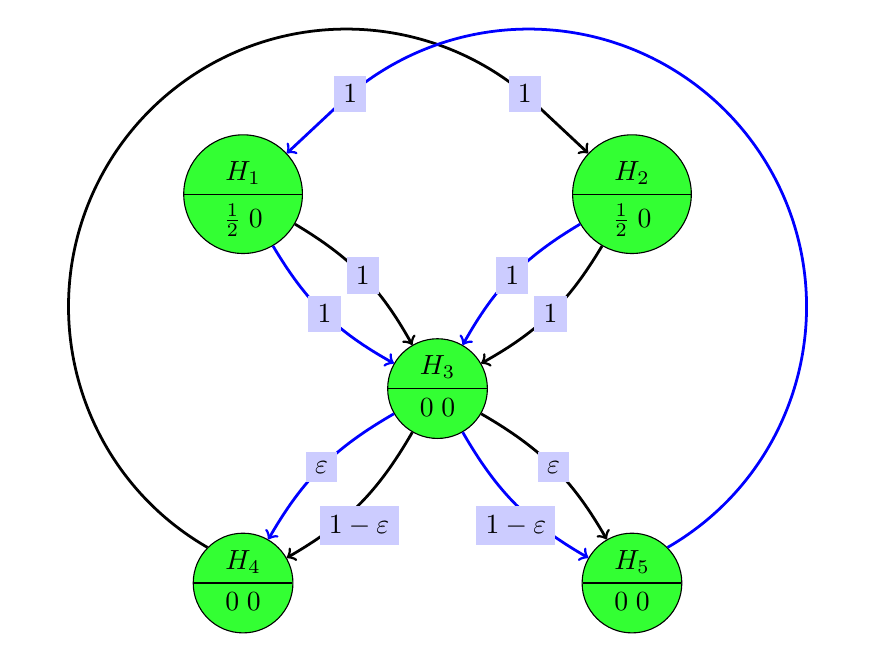
\begin{tikzpicture}[scale=1]
\node (H1) at (70bp,-70bp)[draw,circle split,fill=green!80] {$H_1$ \nodepart{lower} $\frac12\;0$};
\node (H2) at (210bp,-70bp)[draw,circle split,fill=green!80] {$H_2$ \nodepart{lower} $\frac12\;0$};
\node (H3) at (140bp,-140bp)[draw,circle split,fill=green!80] {$H_3$ \nodepart{lower} $0\;0$};
\node (H4) at (70bp,-210bp)[draw,circle split,fill=green!80] {$H_4$ \nodepart{lower} $0\;0$};
\node (H5) at (210bp,-210bp)[draw,circle split,fill=green!80] {$H_5$ \nodepart{lower} $0\;0$};
\draw [draw=black,->,line width=1pt] (H1) to[bend left=15] node[midway,fill=blue!20] {$1$} (H3);
\draw [draw=black,->,line width=1pt] (H2) to[bend left=15] node[midway,fill=blue!20] {$1$} (H3);
\draw [draw=black,->,line width=1pt] (H3) to[bend left=15] node[midway,below,fill=blue!20] {$1-\epsilon$} (H4);
\draw [draw=black,->,line width=1pt] (H3) to[bend left=15] node[midway,fill=blue!20] {$\epsilon$} (H5);
\draw [draw=black,->,line width=1pt] (H4.135) arc(-120:-310:100bp) node[fill=blue!20] {$1$} to (H2);
\draw [draw=blue,->,line width=1pt] (H1) to[bend right=15] node[midway,fill=blue!20] {$1$} (H3);
\draw [draw=blue,->,line width=1pt] (H2) to[bend right=15] node[midway,fill=blue!20] {$1$} (H3);
\draw [draw=blue,->,line width=1pt] (H3) to[bend right=15] node[midway,fill=blue!20] {$\epsilon$} (H4);
\draw [draw=blue,->,line width=1pt] (H3) to[bend right=15] node[midway,below,fill=blue!20] {$1-\epsilon$} (H5);
\draw [draw=blue,->,line width=1pt] (H5.45) arc(-60:130:100bp) node[fill=blue!20] {$1$} to (H1);
\end{tikzpicture}

%<<echo=FALSE,results=tex>>=
%
%cat(graph2latex(Entangled1Maurer2012(), scale=0.7, scaleText=FALSE))
%
%@
  \caption{\label{entagledgraph} Entangled graph from Maurer et Bretz}
\end{figure}

\section{Power Simulations}\index{power simulation}

\subsection{Using the R command line}

\begin{knitrout}\footnotesize
\definecolor{shadecolor}{rgb}{0.969, 0.969, 0.969}\color{fgcolor}\begin{kframe}
\begin{alltt}
\hlcom{# Bonferroni adjustment}
\hlstd{G} \hlkwb{<-} \hlkwd{diag}\hlstd{(}\hlnum{2}\hlstd{)}
\hlstd{weights} \hlkwb{<-} \hlkwd{c}\hlstd{(}\hlnum{0.5}\hlstd{,}\hlnum{0.5}\hlstd{)}
\hlstd{corMat} \hlkwb{<-} \hlkwd{diag}\hlstd{(}\hlnum{2}\hlstd{)}\hlopt{+}\hlkwd{matrix}\hlstd{(}\hlnum{1}\hlstd{,}\hlnum{2}\hlstd{,}\hlnum{2}\hlstd{)}
\hlstd{theta} \hlkwb{<-} \hlkwd{c}\hlstd{(}\hlnum{1}\hlstd{,}\hlnum{2}\hlstd{)}
\hlkwd{calcPower}\hlstd{(weights,} \hlkwc{alpha}\hlstd{=}\hlnum{0.025}\hlstd{, G, theta, corMat)}
\end{alltt}
\begin{verbatim}
## [1] 1 2
##      [,1] [,2]
## [1,]    2    1
## [2,]    1    2
## [1] 10000
## $LocalPower
##     H1     H2 
## 0.1898 0.4322 
## 
## $ExpRejections
## [1] 0.622
## 
## $PowAtlst1
## [1] 0.4837
## 
## $RejectAll
## [1] 0.1383
\end{verbatim}
\begin{alltt}
\hlkwd{calcPower}\hlstd{(weights,} \hlkwc{alpha}\hlstd{=}\hlnum{0.025}\hlstd{, G,} \hlnum{2}\hlopt{*}\hlstd{theta,} \hlnum{2}\hlopt{*}\hlstd{corMat)}
\end{alltt}
\begin{verbatim}
## [1] 2 4
##      [,1] [,2]
## [1,]    4    2
## [2,]    2    4
## [1] 10000
## $LocalPower
##     H1     H2 
## 0.4520 0.8104 
## 
## $ExpRejections
## [1] 1.262
## 
## $PowAtlst1
## [1] 0.8436
## 
## $RejectAll
## [1] 0.4188
\end{verbatim}
\end{kframe}
\end{knitrout}


\begin{figure}[ht]
  \centering
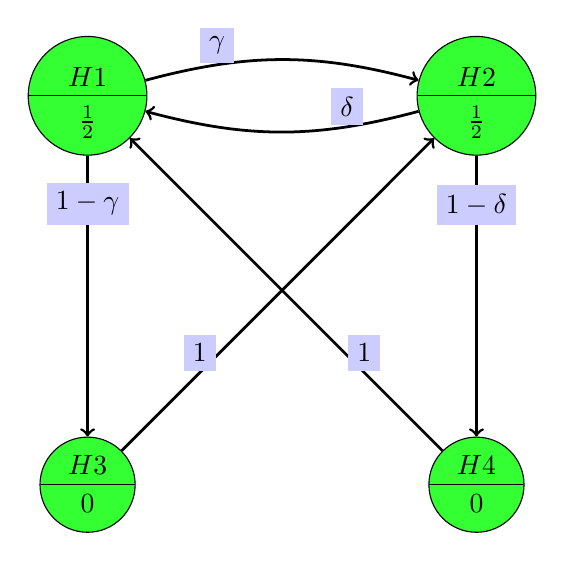
\begin{tikzpicture}[scale=0.7]

\node (H1) at (135.714285714286bp,-135.714285714286bp)[draw,circle split,fill=green!80] {$H1$ \nodepart{lower} $\frac{1}{2}$};
\node (H2) at (335.714285714286bp,-135.714285714286bp)[draw,circle split,fill=green!80] {$H2$ \nodepart{lower} $\frac{1}{2}$};
\node (H3) at (135.714285714286bp,-335.714285714286bp)[draw,circle split,fill=green!80] {$H3$ \nodepart{lower} $0$};
\node (H4) at (335.714285714286bp,-335.714285714286bp)[draw,circle split,fill=green!80] {$H4$ \nodepart{lower} $0$};
\draw [->,line width=1pt] (H1) to[bend left=15] node[near start,above,fill=blue!20] {$\gamma$} (H2);
\draw [->,line width=1pt] (H1) to[auto] node[near start,above,fill=blue!20] {$1-\gamma$} (H3);
\draw [->,line width=1pt] (H2) to[bend left=15] node[near start,above,fill=blue!20] {$\delta$} (H1);
\draw [->,line width=1pt] (H2) to[auto] node[near start,above,fill=blue!20] {$1-\delta$} (H4);
\draw [->,line width=1pt] (H3) to[auto] node[near start,above,fill=blue!20] {$1$} (H2);
\draw [->,line width=1pt] (H4) to[auto] node[near start,above,fill=blue!20] {$1$} (H1);
\end{tikzpicture}


  \caption{\label{powergraph} Graph from Bretz et al. (2009)}
\end{figure}

\begin{figure}[ht]
  \centering    
  \includegraphics[width=9cm]{pictures/power.png}      
  \caption{\label{power} Local power and some (trivial) user defined power functions.}
\end{figure}

\subsection{Variable edge weights}\index{edge weights!variable}

Apart from latin letters the following greek letters can be used to
name a variable\footnote{Note that omicron is not allowed since it can
not be destinguished from the latin character "o".}. Please enter them
with a leading backslash so that they are recognized:

\begin{quote}
  $\backslash$alpha, $\backslash$beta, $\backslash$gamma,
  $\backslash$delta, $\backslash$epsilon, $\backslash$zeta,
  $\backslash$eta, $\backslash$theta, $\backslash$iota,
  $\backslash$kappa, $\backslash$lambda, $\backslash$mu,
  $\backslash$nu, $\backslash$xi,
  % $\backslash$omicron,
  $\backslash$pi, $\backslash$rho, $\backslash$sigma, $\backslash$tau,
  $\backslash$upsilon, $\backslash$phi, $\backslash$chi,
  $\backslash$psi, $\backslash$omega.
\end{quote}

These are shown in the GUI as $\alpha,\; \beta,\; \gamma,\; \delta,\;
\epsilon,\; \zeta,\; \eta,\; \theta,\; \iota,\; \kappa,\; \lambda,\;
\mu,\; \nu,\; \xi,\;
%\omicron,\; 
\pi,\; \rho,\; \sigma,\; \tau,\; \upsilon,\; \phi, \chi,\; \psi$ and
$\omega$.

\includegraphics[width=5cm]{pictures/variableEditor.png}

\begin{knitrout}\footnotesize
\definecolor{shadecolor}{rgb}{0.969, 0.969, 0.969}\color{fgcolor}\begin{kframe}
\begin{alltt}
\hlstd{graph} \hlkwb{<-} \hlkwd{generalSuccessive}\hlstd{()}
\hlstd{graph}
\end{alltt}
\begin{verbatim}
## A graphMCP graph
## H1 (weight=0.5)
## H2 (weight=0.5)
## H3 (weight=0)
## H4 (weight=0)
## Edges:
## H1  -( \gamma )->  H2 
## H1  -( 1-\gamma )->  H3 
## H2  -( \delta )->  H1 
## H2  -( 1-\delta )->  H4 
## H3  -( 1 )->  H2 
## H4  -( 1 )->  H1
\end{verbatim}
\end{kframe}
\end{knitrout}


\section{Options and Import/Export}

\subsection{Options}\index{options}

\begin{description}
  \item[Grid] For easier placement of nodes a grid can be used that aligns the
  nodes to its intersections. You can specify a positive integer that sets the
  grid size, i.e.\ the width in pixels between two proximate parallel
  lines. If you set the grid size to 1 this would allow unrestricted placement
  and therefore disables the grid.
  \item[Number of digits] Number of digits to be shown at various places. In
  this version not every part of the GUI will use this value, but this will
  improve in further versions.
  \item[Line width] Especially if you want to use exported PNG graphics in
    other documents, you may want to adjust the line width of edges and nodes,
    when borders look to thin or thick.
  \item[Font Size] Font size of the text in the GUI widgets.
  \item[Look'n'Feel] The way the widgets of a GUI look and how they behave
    is called "look and feel" in Java. Depending on your operating
    system and classpath several Look'n'Feel implementations may be available 
    (e.g. Metal (Java default), Windows, Mac OS, Motif and/or System/GTK).
    If you are used to a particular Look'n'Feel, you can select it here.
    But if you have problems with the graphical interface, please try to use
    the default Metal theme to check whether it could be a problem with the
    selected Look'n'Feel.
  \item[Colored image files and pdf reports] Colors are used to highlight
    different conditions in the graph like hypotheses that could be rejected.
    While these colors are helpful in the GUI, you perhaps prefer black and
    white PNG image files and PDF reports.
  \item[Show rejected nodes in GUI] When using the GUI to for stepwise rejection
    of hypotheses, this options determines whether rejected nodes should
    "disappear" or whether they remain on the screen and are only marked as
    rejected.
  \item[Use JLaTeXMath] There are not many reasons not to use the free Java
    library JLaTeXMath to render numbers, symbols and formulas in the
    GUI. The option is mainly provided in case that errors occur
    displaying the numbers and formulas.
  \item[Show epsilon edges as dashed lines] You can set whether epsilon
    edges should been shown as dashed or solid lines.
  \item[Show fractions instead of decimal numbers] Floating point numbers are used
    for all calculations and values like $1/3$ would be normally shown as
    $0.3333333$. When this option is active the method fractions from package
    MASS is used to display fractions whenever the floating point numbers are
    close to a fraction that looks right.  
  \item[Use epsilon approximation] In this version this value can not be
    changed. No calculations with infinitesimal small values are done but
    instead the epsilon is approximated by a small real number.
  \item[Epsilon] The small real value that should be used to approximate
    the infinitesimal small epsilon. Default is $10^{-3}$.
%  \item[Try to show fractions / rounded numbers] Floating point numbers are
%   used for all calculations and values like $1/3$ would be normally shown as
%    $0.3333333$. When this option is active the method fractions from package
%    MASS is used to display fractions whenever the floating point numbers are
%    close to a fraction that looks right.
%  \item[Number of digits to assure] This is an option for displaying numbers
%  and does not influence the calculations. As seen in the previous option
%  description, we sometimes try to display fractions instead of floating point
%  numbers. This option will assure that the shown fraction does not
%  differ in more than the specified value from the floating point number.
  \item[Verbose output of algorithms] If checked the selected the algorithms produce a
  verbose output that is shown in the GUI. For example the Simes test specifies
  for each intersection of elementar hypotheses whether and why it could be
  rejected.
  \item[Monte Carlo sample size for power] The Monte Carlo sample size for power
  calculations. Default is 10000.
  \item[Type of random numbers] You can select quasirandom or pseudorandom
  numbers for power calculations. The quasirandom option uses a randomized
  Lattice rule, and should be more efficient than the pseudorandom option that
  uses ordinary (pseudo) random numbers.
  \item[Check online for updates] On start-up gMCP can check automatically
    whether a new version of gMCP is available. Only your version of R (like
    2.13.1), the version of gMCP (like 0.7-5) and a random number (to
    distinguish different requests) are transmitted.
  \item[Weights of subgraphs are upscaled to 1] If '\emph{No}' is selected then 
    for each intersection of hypotheses (i.e. each subgraph)
    a weighted test is performed at the possibly reduced level alpha of $\text{sum}(w)*alpha$,
    where $\text{sum}(w)$ is the sum of all node weights in this subset
    If '\emph{Yes}' is selected all weights are upscaled, so that $\text{sum}(w)=1$.
  \item[Export images with transparent background] If checked the background of
    exported PNG graphics will be transparent. Otherwise the graphs are
    displayed on a white background.
  \item[If a node is dragged also all edges to this node follow] If selected the
    edges will always repositioned whenever a node is dragged. Otherwise only
    newly added eges behave that way and edges that have been dragged themselves
    are considered "anchored" and will stay with the edge weight label at the
    same position.
  \item[Automatically enter the editing mode, whenever a table cell
    gets the focus] 
  \item[Enable highly experimental feature]\label{experimentalFeatures} The gMCP
    GUI often contains new features that are not that well tested. If you want
    to use or take a look at them, activate this option. But be prepared that
    things might go wrong.
  \item[Show R code to reproduce results in R] After performing a test in the GUI 
    the result dialog does not only show the pure results, but also R code to 
    reproduce these results in R. If you are not interested in this feature
    you can disable it here.
\end{description}

\subsubsection{Privacy}

The GUI always asks before sending data to our server. It will do so to
\begin{enumerate}
  \item check whether a new version of gMCP exists,  
%  \item send a wishlist if the user chooses to,
  \item submit/load a graph to the online archive 
  \item send bug reports if an error occurs.
\end{enumerate}

Only in the last case of a bug report some information about your
computer is collected that can be reviewed by the user before sending
the bug report. If you do not agree with sending this data, simply
don't send a problematic bug report or if you never want to send bug
reports, disable the option in the options menu.

\subsection{Import/Exports}\index{import}\index{export}

This subsection is work in progress, but fortunately the menu entries
in figure \ref{fig:fileMenu} should be fairly self-explanatory.

\begin{figure}[ht]
  \centering    
  \includegraphics[width=4cm]{pictures/filemenu.png}      
  \caption{\label{fig:fileMenu} Import and export of graphs.}
\end{figure}

You can export graphs to png files. The background of these png files
will be made transparent, so that they will fit into whichever
document you insert them.  Note that some image viewers visualize
transparency with a checkerboard pattern. In some Windows application
the transparent background may be wrongly shown as black - if this
happens or you generally prefer a non-transparent white background,
you can toggle the option "\emph{Export images with transparent 
background}" in the options dialog.

Since version 0.8-7 gMCP also can create word documents (Office Open XML / docx).

\begin{figure}[ht]
  \centering    
  \includegraphics[width=7cm]{pictures/docxExport.png}      
  \caption{\label{fig:wordexample} Example Word export - first page.}
\end{figure}

\subsection{Important TikZ commands for optimizing the reports}\index{graph2latex}\index{TikZ}
A clear automatic placement of edges and weight labels without
overlapping is a very difficult task and for complicated graphs the
\texttt{gMCP} package will often fail to accomplish this
automatically. If the result of \texttt{graph2latex} does not give you
an acceptable layout, simply load the graph into the GUI and use the
mouse to drag the edge labels around until you are satisfied with the
placement. Save the graph and the TikZ output will be pretty close to
the graph seen in the GUI.

PGF/TikZ is very useful \LaTeX-package, we recommend it for many
purposes and it's totally worth reading its 560 pages manual
(\cite{TikZ}), but if you don't have the time right now, we will give
you short overview of the most important commands for our kind of
graphs so that you can easily adapt the output from
\texttt{graph2latex}.

You also perhaps want to use an TikZ editor with a preview pane like qtikz
or
ktikz\footnote{\url{http://www.hackenberger.at/blog/ktikz-editor-for-the-tikz-language/}}.

Let's start with this graph in figure \ref{uglygraph}:

\scriptsize
\lstset{language=[LaTeX]TeX}
\begin{lstlisting}
\begin{tikzpicture}[scale=1]
\node (H11) at (200bp,200bp) [draw,circle split,fill=green!80] {$H11$ \nodepart{lower} $0.0333$};
...
\draw [->,line width=1pt] (H11) to[bend left=15] node[near start,above,fill=blue!20] {0.667} (H12);
...
\end{tikzpicture}
\end{lstlisting}
\normalsize

\begin{figure}[ht]
  \centering
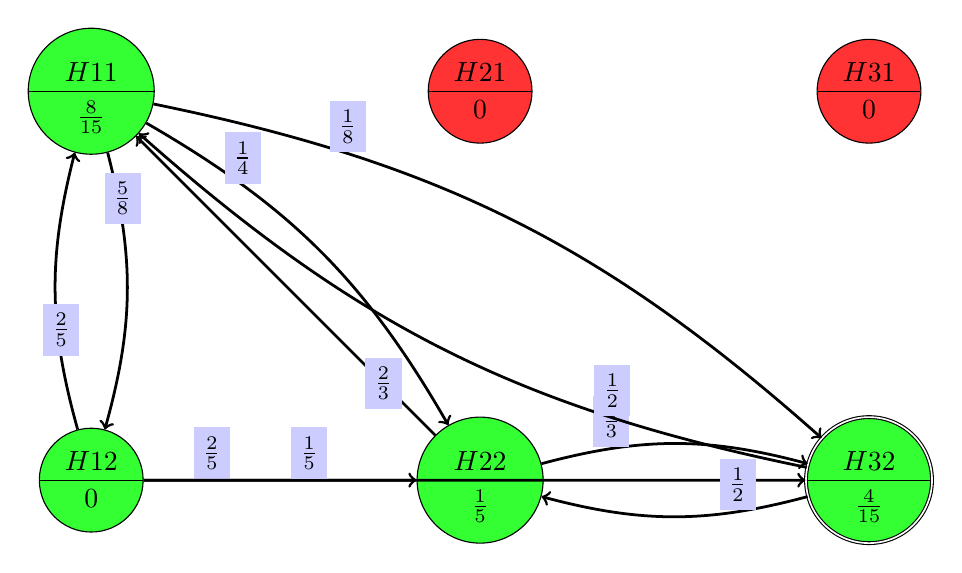
\begin{tikzpicture}[scale=0.7]

\node (H11) at (135.714285714286bp,-135.714285714286bp)[draw,circle split,fill=green!80] {$H11$ \nodepart{lower} $\frac{8}{15}$};
\node (H21) at (335.714285714286bp,-135.714285714286bp)[draw,circle split,fill=red!80] {$H21$ \nodepart{lower} $0$};
\node (H31) at (535.714285714286bp,-135.714285714286bp)[draw,circle split,fill=red!80] {$H31$ \nodepart{lower} $0$};
\node (H12) at (135.714285714286bp,-335.714285714286bp)[draw,circle split,fill=green!80] {$H12$ \nodepart{lower} $0$};
\node (H22) at (335.714285714286bp,-335.714285714286bp)[draw,circle split,fill=green!80] {$H22$ \nodepart{lower} $\frac{1}{5}$};
\node (H32) at (535.714285714286bp,-335.714285714286bp)[draw,circle split,double,fill=green!80] {$H32$ \nodepart{lower} $\frac{4}{15}$};
\draw [->,line width=1pt] (H11) to[bend left=15] node[near start,above,fill=blue!20] {$\frac{5}{8}$} (H12);
\draw [->,line width=1pt] (H11) to[bend left=15] node[near start,above,fill=blue!20] {$\frac{1}{4}$} (H22);
\draw [->,line width=1pt] (H11) to[bend left=15] node[near start,above,fill=blue!20] {$\frac{1}{8}$} (H32);
\draw [->,line width=1pt] (H12) to[bend left=15] node[near start,above,fill=blue!20] {$\frac{2}{5}$} (H11);
\draw [->,line width=1pt] (H12) to[auto] node[near start,above,fill=blue!20] {$\frac{2}{5}$} (H22);
\draw [->,line width=1pt] (H12) to[auto] node[near start,above,fill=blue!20] {$\frac{1}{5}$} (H32);
\draw [->,line width=1pt] (H22) to (286bp, -286bp) node[fill=blue!20] {$\frac{2}{3}$} to (H11);
\draw [->,line width=1pt] (H22) to[bend left=15] node[near start,above,fill=blue!20] {$\frac{1}{3}$} (H32);
\draw [->,line width=1pt] (H32) to[bend left=15] node[near start,above,fill=blue!20] {$\frac{1}{2}$} (H11);
\draw [->,line width=1pt] (H32) to[bend left=15] node[near start,above,fill=blue!20] {$\frac{1}{2}$} (H22);
\end{tikzpicture}


  \caption{\label{uglygraph}Graph from \texttt{graph2latex} that does not look optimal.}
\end{figure}

You can scale the TikZ graphic by changing the \texttt{[scale=1]}
option.  By default \texttt{graph2latex} doesn't scale TikZ graphics,
but has an optional parameter \texttt{scale}.

For an explanation what \texttt{green!80} means and how you can
specify other colors, please take a look at the xcolor manual
from \cite{xcolor}.

You can choose between the following label positions \texttt{above,
  below, right, left, above right, above left, below right}, and
\texttt{below left}.  In addition these positions can take an optional
dimension argument, so that for example \texttt{below=1pt} can be used
to place a label below and additionally shift it 1pt downwards.

You can change the position where the edge weight label is placed to
\texttt{at start, very near start, near start, midway, near end, very
  near end} and \texttt{at end} or simply use something like
\texttt{pos=0.5}.  If you add an argument \texttt{sloped}, the text
label will be rotated so that a parallel line to the base line becomes
a tangent to the edge.

Often it is useful to reduce the bending angle in \texttt{[bend
    left=15]} below 15. You could also specify and change
\texttt{out=15} and \texttt{in=165} separately.

A powerful feature is the use of styles, since this will effect all
objects of a given class. But for this please take a look directly at
the TikZ manual (\cite{TikZ}).

\section{Case Studies}\label{sec:caseStudies}

This section is work in progress.

\subsection{Identifying effective and/or safe doses by stepwise confidence intervals for ratios}
In this subsection we show how to use gMCP to reproduce the results of the paper from \cite{bretz2003identifying} with the same title.

\subsection{Testing strategies in multi-dose experiments including active control}

\cite{bauer1998testing}

\begin{knitrout}\footnotesize
\definecolor{shadecolor}{rgb}{0.969, 0.969, 0.969}\color{fgcolor}\begin{kframe}
\begin{alltt}
\hlkwd{data}\hlstd{(hydroquinone)}
\hlstd{pvalues} \hlkwb{<-} \hlkwd{c}\hlstd{()}
\hlstd{x} \hlkwb{<-} \hlstd{hydroquinone}\hlopt{$}\hlstd{micronuclei[hydroquinone}\hlopt{$}\hlstd{group} \hlopt{==} \hlstr{"C-"}\hlstd{]}
\hlkwa{for} \hlstd{(dose} \hlkwa{in} \hlkwd{c}\hlstd{(}\hlstr{"30 mg/kg"}\hlstd{,} \hlstr{"50 mg/kg"}\hlstd{,} \hlstr{"75 mg/kg"}\hlstd{,} \hlstr{"100 mg/kg"}\hlstd{,} \hlstr{"C+"}\hlstd{)) \{}
    \hlstd{y} \hlkwb{<-} \hlstd{hydroquinone}\hlopt{$}\hlstd{micronuclei[hydroquinone}\hlopt{$}\hlstd{group} \hlopt{==} \hlstd{dose]}
    \hlstd{result} \hlkwb{<-} \hlkwd{wilcox.test}\hlstd{(x, y,} \hlkwc{alternative} \hlstd{=} \hlstr{"less"}\hlstd{,} \hlkwc{correct} \hlstd{=} \hlnum{TRUE}\hlstd{)}
    \hlstd{pvalues} \hlkwb{<-} \hlkwd{c}\hlstd{(result}\hlopt{$}\hlstd{p.value, pvalues)}
\hlstd{\}}
\hlstd{pvalues}
\end{alltt}
\begin{verbatim}
## [1] 0.004929 0.002634 0.002634 0.004319 0.066255
\end{verbatim}
\begin{alltt}
\hlkwd{library}\hlstd{(coin,} \hlkwc{quietly} \hlstd{=} \hlnum{TRUE}\hlstd{)}
\hlstd{pvalues} \hlkwb{<-} \hlkwd{c}\hlstd{()}
\hlkwa{for} \hlstd{(dose} \hlkwa{in} \hlkwd{c}\hlstd{(}\hlstr{"30 mg/kg"}\hlstd{,} \hlstr{"50 mg/kg"}\hlstd{,} \hlstr{"75 mg/kg"}\hlstd{,} \hlstr{"100 mg/kg"}\hlstd{,} \hlstr{"C+"}\hlstd{)) \{}
    \hlstd{subdata} \hlkwb{<-} \hlkwd{droplevels}\hlstd{(hydroquinone[hydroquinone}\hlopt{$}\hlstd{group} \hlopt \hlkwd{c}\hlstd{(}\hlstr{"C-"}\hlstd{, dose), ])}
    \hlstd{result} \hlkwb{<-} \hlkwd{wilcox_test}\hlstd{(micronuclei} \hlopt{~} \hlstd{group,} \hlkwc{data} \hlstd{= subdata,} \hlkwc{distribution} \hlstd{=} \hlstr{"exact"}\hlstd{)}
    \hlstd{pvalues} \hlkwb{<-} \hlkwd{c}\hlstd{(}\hlkwd{pvalue}\hlstd{(result), pvalues)}
\hlstd{\}}
\hlstd{pvalues}
\end{alltt}
\begin{verbatim}
## [1] 0.006061 0.001263 0.001263 0.005051 0.135101
\end{verbatim}
\end{kframe}
\end{knitrout}


\begin{figure}[ht]
\begin{center}
\begin{knitrout}\footnotesize
\definecolor{shadecolor}{rgb}{0.969, 0.969, 0.969}\color{fgcolor}
\includegraphics[width=\maxwidth]{figure/unnamed-chunk-25} 

\end{knitrout}

\end{center}
\caption{\label{bpHydroquinone} Boxplot of the hydroquinone data set}
\end{figure}

\clearpage

\begin{appendix} 

\section{Appendix - Example graphs}\label{sec:exampleGraphs}

\begin{figure}[ht]
\begin{center}
\scalebox{0.7}{
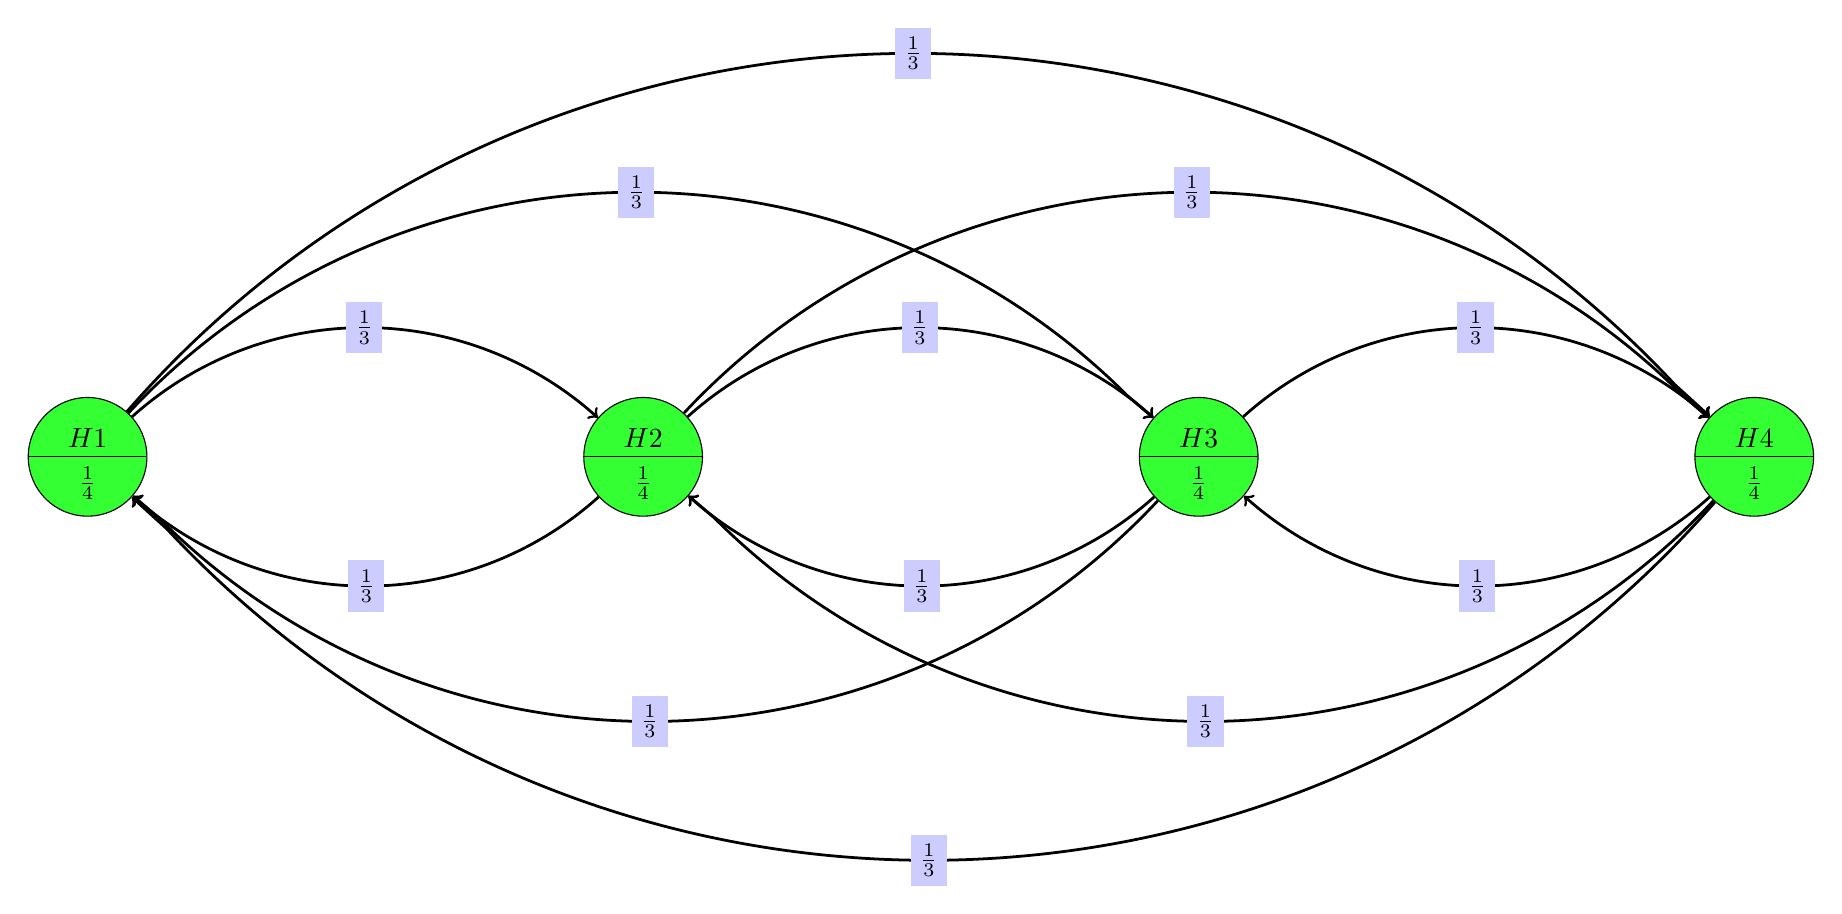
\begin{tikzpicture}

\node (H1) at (125bp,-225bp)[draw,circle split,fill=green!80] {$H1$ \nodepart{lower} $\frac{1}{4}$};
\node (H2) at (325bp,-225bp)[draw,circle split,fill=green!80] {$H2$ \nodepart{lower} $\frac{1}{4}$};
\node (H3) at (525bp,-225bp)[draw,circle split,fill=green!80] {$H3$ \nodepart{lower} $\frac{1}{4}$};
\node (H4) at (725bp,-225bp)[draw,circle split,fill=green!80] {$H4$ \nodepart{lower} $\frac{1}{4}$};
\draw [->,line width=1pt] (H1.42) arc(132:90:125bp) node[fill=blue!20] {$\frac{1}{3}$} arc(90:50:125bp) to (H2);
\draw [->,line width=1pt] (H1.47) arc(137:90:250bp) node[fill=blue!20] {$\frac{1}{3}$} arc(90:45:250bp) to (H3);
\draw [->,line width=1pt] (H1.49) arc(139:90:375bp) node[fill=blue!20] {$\frac{1}{3}$} arc(90:43:375bp) to (H4);
\draw [->,line width=1pt] (H2.222) arc(312:270:125bp) node[fill=blue!20] {$\frac{1}{3}$} arc(270:230:125bp) to (H1);
\draw [->,line width=1pt] (H2.42) arc(132:90:125bp) node[fill=blue!20] {$\frac{1}{3}$} arc(90:50:125bp) to (H3);
\draw [->,line width=1pt] (H2.47) arc(137:90:250bp) node[fill=blue!20] {$\frac{1}{3}$} arc(90:45:250bp) to (H4);
\draw [->,line width=1pt] (H3.227) arc(317:270:250bp) node[fill=blue!20] {$\frac{1}{3}$} arc(270:225:250bp) to (H1);
\draw [->,line width=1pt] (H3.222) arc(312:270:125bp) node[fill=blue!20] {$\frac{1}{3}$} arc(270:230:125bp) to (H2);
\draw [->,line width=1pt] (H3.42) arc(132:90:125bp) node[fill=blue!20] {$\frac{1}{3}$} arc(90:50:125bp) to (H4);
\draw [->,line width=1pt] (H4.229) arc(319:270:375bp) node[fill=blue!20] {$\frac{1}{3}$} arc(270:223:375bp) to (H1);
\draw [->,line width=1pt] (H4.227) arc(317:270:250bp) node[fill=blue!20] {$\frac{1}{3}$} arc(270:225:250bp) to (H2);
\draw [->,line width=1pt] (H4.222) arc(312:270:125bp) node[fill=blue!20] {$\frac{1}{3}$} arc(270:230:125bp) to (H3);
\end{tikzpicture}

}
\end{center}

\end{figure}\begin{figure}[ht]
\begin{center}
\scalebox{0.7}{
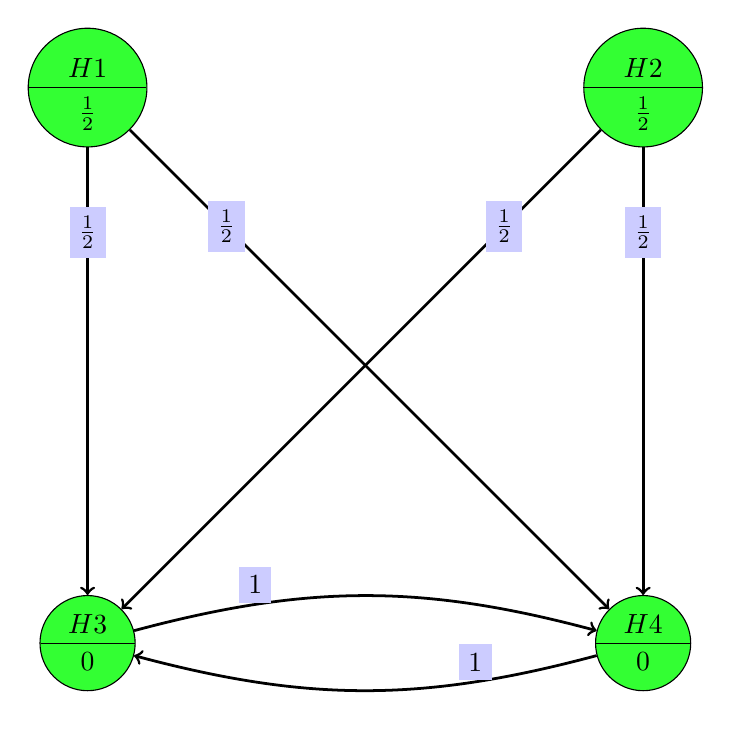
\begin{tikzpicture}

\node (H1) at (125bp,-125bp)[draw,circle split,fill=green!80] {$H1$ \nodepart{lower} $\frac{1}{2}$};
\node (H2) at (325bp,-125bp)[draw,circle split,fill=green!80] {$H2$ \nodepart{lower} $\frac{1}{2}$};
\node (H3) at (125bp,-325bp)[draw,circle split,fill=green!80] {$H3$ \nodepart{lower} $0$};
\node (H4) at (325bp,-325bp)[draw,circle split,fill=green!80] {$H4$ \nodepart{lower} $0$};
\draw [->,line width=1pt] (H1) to[auto] node[near start,above,fill=blue!20] {$\frac{1}{2}$} (H3);
\draw [->,line width=1pt] (H1) to (175bp, -175bp) node[fill=blue!20] {$\frac{1}{2}$} to (H4);
\draw [->,line width=1pt] (H2) to (275bp, -175bp) node[fill=blue!20] {$\frac{1}{2}$} to (H3);
\draw [->,line width=1pt] (H2) to[auto] node[near start,above,fill=blue!20] {$\frac{1}{2}$} (H4);
\draw [->,line width=1pt] (H3) to[bend left=15] node[near start,above,fill=blue!20] {$1$} (H4);
\draw [->,line width=1pt] (H4) to[bend left=15] node[near start,above,fill=blue!20] {$1$} (H3);
\end{tikzpicture}

}
\end{center}

\end{figure}\begin{figure}[ht]
\begin{center}
\scalebox{0.7}{
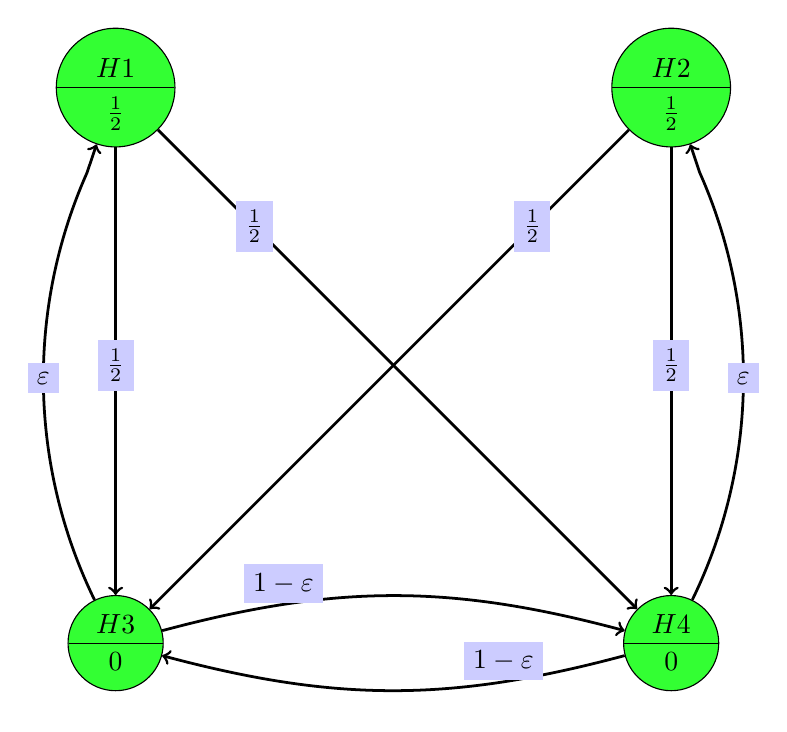
\begin{tikzpicture}

\node (H1) at (125bp,-125bp)[draw,circle split,fill=green!80] {$H1$ \nodepart{lower} $\frac{1}{2}$};
\node (H2) at (325bp,-125bp)[draw,circle split,fill=green!80] {$H2$ \nodepart{lower} $\frac{1}{2}$};
\node (H3) at (125bp,-325bp)[draw,circle split,fill=green!80] {$H3$ \nodepart{lower} $0$};
\node (H4) at (325bp,-325bp)[draw,circle split,fill=green!80] {$H4$ \nodepart{lower} $0$};
\draw [->,line width=1pt] (H1) to (125bp, -225bp) node[fill=blue!20] {$\frac{1}{2}$} to (H3);
\draw [->,line width=1pt] (H1) to (175bp, -175bp) node[fill=blue!20] {$\frac{1}{2}$} to (H4);
\draw [->,line width=1pt] (H2) to (275bp, -175bp) node[fill=blue!20] {$\frac{1}{2}$} to (H3);
\draw [->,line width=1pt] (H2) to (325bp, -225bp) node[fill=blue!20] {$\frac{1}{2}$} to (H4);
\draw [->,line width=1pt] (H3.116) arc(206:180:182bp) node[fill=blue!20] {$\epsilon$} arc(180:156:182bp) to (H1);
\draw [->,line width=1pt] (H3) to[bend left=15] node[near start,above,fill=blue!20] {$1-\epsilon$} (H4);
\draw [->,line width=1pt] (H4.424) arc(334:360:182bp) node[fill=blue!20] {$\epsilon$} arc(360:384:182bp) to (H2);
\draw [->,line width=1pt] (H4) to[bend left=15] node[near start,above,fill=blue!20] {$1-\epsilon$} (H3);
\end{tikzpicture}

}
\end{center}

\end{figure}\begin{figure}[ht]
\begin{center}
\scalebox{0.7}{
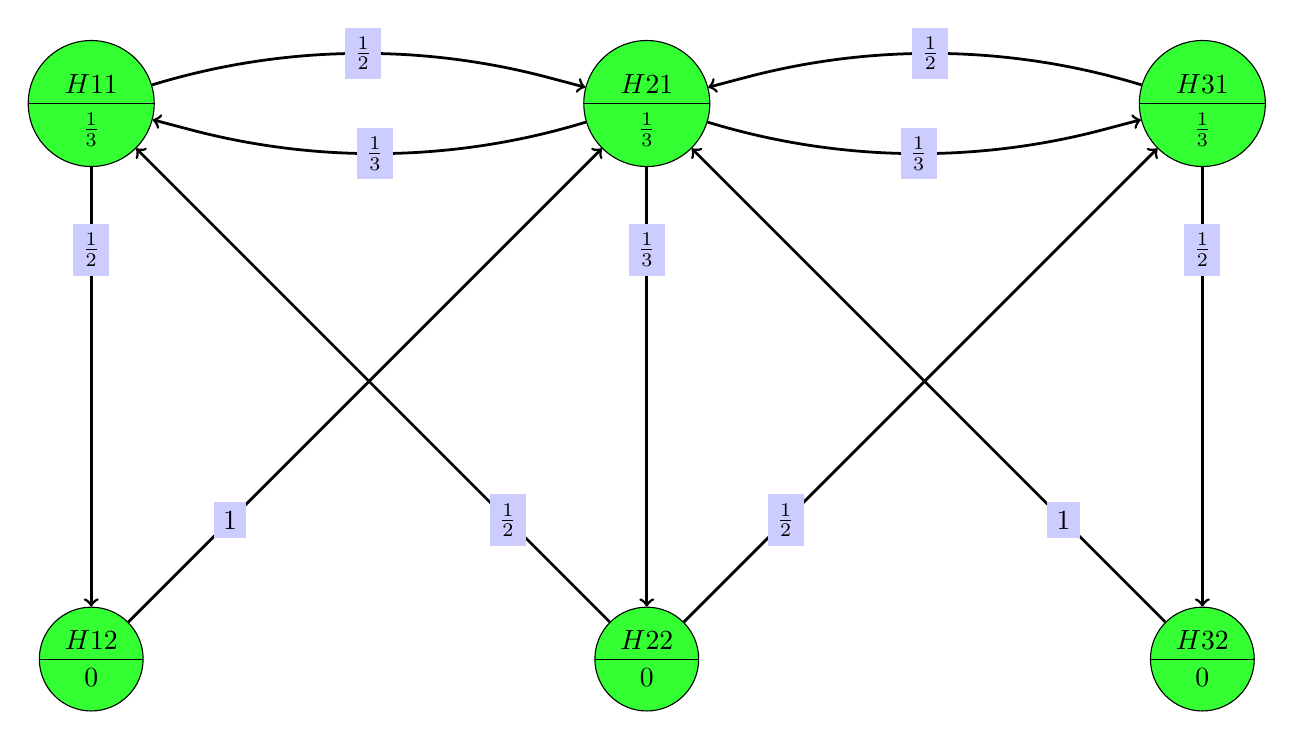
\begin{tikzpicture}

\node (H11) at (125bp,-125bp)[draw,circle split,fill=green!80] {$H11$ \nodepart{lower} $\frac{1}{3}$};
\node (H21) at (325bp,-125bp)[draw,circle split,fill=green!80] {$H21$ \nodepart{lower} $\frac{1}{3}$};
\node (H31) at (525bp,-125bp)[draw,circle split,fill=green!80] {$H31$ \nodepart{lower} $\frac{1}{3}$};
\node (H12) at (125bp,-325bp)[draw,circle split,fill=green!80] {$H12$ \nodepart{lower} $0$};
\node (H22) at (325bp,-325bp)[draw,circle split,fill=green!80] {$H22$ \nodepart{lower} $0$};
\node (H32) at (525bp,-325bp)[draw,circle split,fill=green!80] {$H32$ \nodepart{lower} $0$};
\draw [->,line width=1pt] (H11.17) arc(107:90:260bp) node[fill=blue!20] {$\frac{1}{2}$} arc(90:75:260bp) to (H21);
\draw [->,line width=1pt] (H11) to[auto] node[near start,above,fill=blue!20] {$\frac{1}{2}$} (H12);
\draw [->,line width=1pt] (H21.197) arc(287:270:260bp) node[fill=blue!20] {$\frac{1}{3}$} arc(270:255:260bp) to (H11);
\draw [->,line width=1pt] (H21.343) arc(253:270:260bp) node[fill=blue!20] {$\frac{1}{3}$} arc(270:285:260bp) to (H31);
\draw [->,line width=1pt] (H21) to[auto] node[near start,above,fill=blue!20] {$\frac{1}{3}$} (H22);
\draw [->,line width=1pt] (H31.163) arc(73:90:260bp) node[fill=blue!20] {$\frac{1}{2}$} arc(90:105:260bp) to (H21);
\draw [->,line width=1pt] (H31) to[auto] node[near start,above,fill=blue!20] {$\frac{1}{2}$} (H32);
\draw [->,line width=1pt] (H12) to (175bp, -275bp) node[fill=blue!20] {$1$} to (H21);
\draw [->,line width=1pt] (H22) to (275bp, -275bp) node[fill=blue!20] {$\frac{1}{2}$} to (H11);
\draw [->,line width=1pt] (H22) to (375bp, -275bp) node[fill=blue!20] {$\frac{1}{2}$} to (H31);
\draw [->,line width=1pt] (H32) to (475bp, -275bp) node[fill=blue!20] {$1$} to (H21);
\end{tikzpicture}

}
\end{center}

\end{figure}\begin{figure}[ht]
\begin{center}
\scalebox{0.7}{
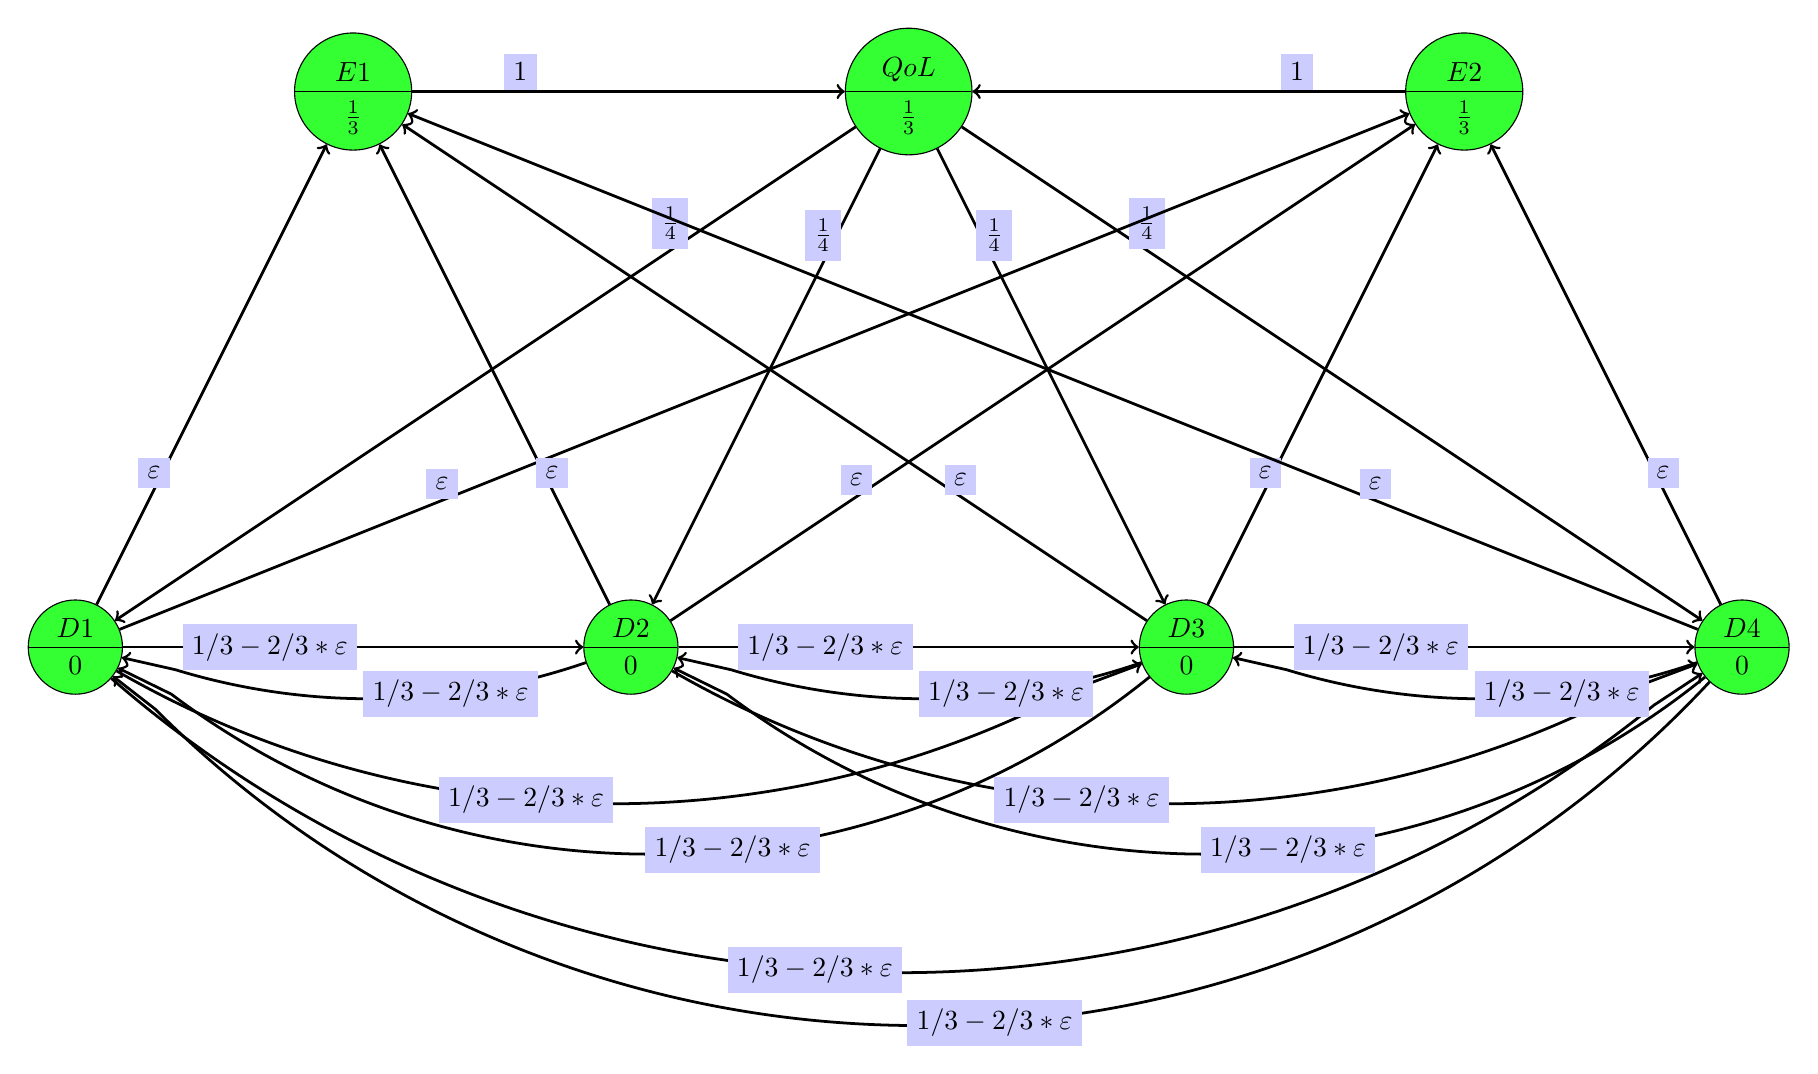
\begin{tikzpicture}

\node (E1) at (225bp,-125bp)[draw,circle split,fill=green!80] {$E1$ \nodepart{lower} $\frac{1}{3}$};
\node (QoL) at (425bp,-125bp)[draw,circle split,fill=green!80] {$QoL$ \nodepart{lower} $\frac{1}{3}$};
\node (E2) at (625bp,-125bp)[draw,circle split,fill=green!80] {$E2$ \nodepart{lower} $\frac{1}{3}$};
\node (D1) at (125bp,-325bp)[draw,circle split,fill=green!80] {$D1$ \nodepart{lower} $0$};
\node (D2) at (325bp,-325bp)[draw,circle split,fill=green!80] {$D2$ \nodepart{lower} $0$};
\node (D3) at (525bp,-325bp)[draw,circle split,fill=green!80] {$D3$ \nodepart{lower} $0$};
\node (D4) at (725bp,-325bp)[draw,circle split,fill=green!80] {$D4$ \nodepart{lower} $0$};
\draw [->,line width=1pt] (E1) to[auto] node[near start,above,fill=blue!20] {$1$} (QoL);
\draw [->,line width=1pt] (QoL) to[auto] node[near start,above,fill=blue!20] {$\frac{1}{4}$} (D1);
\draw [->,line width=1pt] (QoL) to[auto] node[near start,above,fill=blue!20] {$\frac{1}{4}$} (D2);
\draw [->,line width=1pt] (QoL) to[auto] node[near start,above,fill=blue!20] {$\frac{1}{4}$} (D3);
\draw [->,line width=1pt] (QoL) to[auto] node[near start,above,fill=blue!20] {$\frac{1}{4}$} (D4);
\draw [->,line width=1pt] (E2) to[auto] node[near start,above,fill=blue!20] {$1$} (QoL);
\draw [->,line width=1pt] (D1) to[auto] node[near start,above,fill=blue!20] {$\epsilon$} (E1);
\draw [->,line width=1pt] (D1) to[auto] node[near start,above,fill=blue!20] {$\epsilon$} (E2);
\draw [->,line width=1pt] (D1) to (195bp, -325bp) node[fill=blue!20] {$1/3-2/3*\epsilon$} to (D2);
\draw [->,line width=1pt] (D1.330) arc(240:265:357bp) node[fill=blue!20] {$1/3-2/3*\epsilon$} arc(265:298:357bp) to (D3);
\draw [->,line width=1pt] (D1.319) arc(229:266:432bp) node[fill=blue!20] {$1/3-2/3*\epsilon$} arc(266:309:432bp) to (D4);
\draw [->,line width=1pt] (D2) to[auto] node[near start,above,fill=blue!20] {$\epsilon$} (E1);
\draw [->,line width=1pt] (D2) to[auto] node[near start,above,fill=blue!20] {$\epsilon$} (E2);
\draw [->,line width=1pt] (D2.199) arc(289:277:239bp) node[fill=blue!20] {$1/3-2/3*\epsilon$} arc(277:253:239bp) to (D1);
\draw [->,line width=1pt] (D2) to (395bp, -325bp) node[fill=blue!20] {$1/3-2/3*\epsilon$} to (D3);
\draw [->,line width=1pt] (D2.330) arc(240:265:357bp) node[fill=blue!20] {$1/3-2/3*\epsilon$} arc(265:298:357bp) to (D4);
\draw [->,line width=1pt] (D3) to[auto] node[near start,above,fill=blue!20] {$\epsilon$} (E1);
\draw [->,line width=1pt] (D3) to[auto] node[near start,above,fill=blue!20] {$\epsilon$} (E2);
\draw [->,line width=1pt] (D3.219) arc(309:276:286bp) node[fill=blue!20] {$1/3-2/3*\epsilon$} arc(276:233:286bp) to (D1);
\draw [->,line width=1pt] (D3.199) arc(289:277:239bp) node[fill=blue!20] {$1/3-2/3*\epsilon$} arc(277:253:239bp) to (D2);
\draw [->,line width=1pt] (D3) to (595bp, -325bp) node[fill=blue!20] {$1/3-2/3*\epsilon$} to (D4);
\draw [->,line width=1pt] (D4) to[auto] node[near start,above,fill=blue!20] {$\epsilon$} (E1);
\draw [->,line width=1pt] (D4) to[auto] node[near start,above,fill=blue!20] {$\epsilon$} (E2);
\draw [->,line width=1pt] (D4.227) arc(317:274:389bp) node[fill=blue!20] {$1/3-2/3*\epsilon$} arc(274:225:389bp) to (D1);
\draw [->,line width=1pt] (D4.219) arc(309:276:286bp) node[fill=blue!20] {$1/3-2/3*\epsilon$} arc(276:233:286bp) to (D2);
\draw [->,line width=1pt] (D4.199) arc(289:277:239bp) node[fill=blue!20] {$1/3-2/3*\epsilon$} arc(277:253:239bp) to (D3);
\end{tikzpicture}

}
\end{center}

\end{figure}\begin{figure}[ht]
\begin{center}
\scalebox{0.7}{
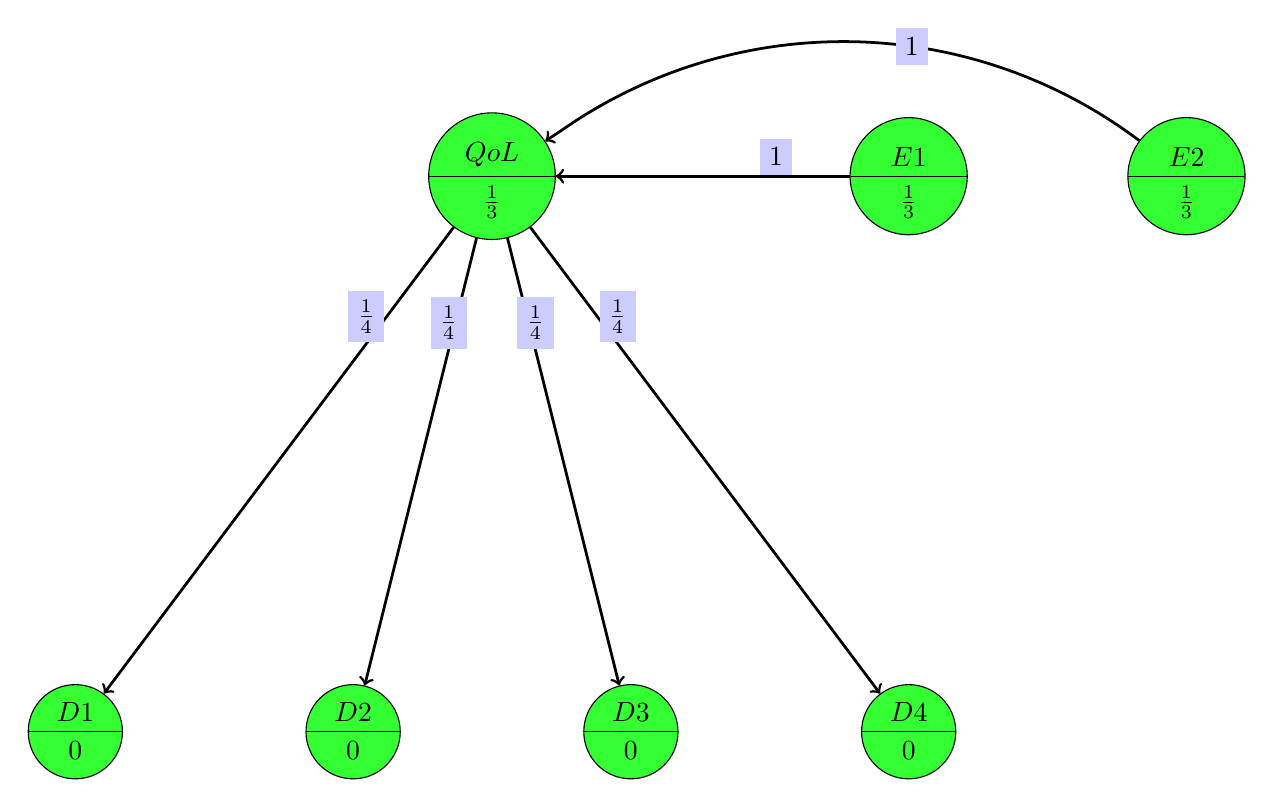
\begin{tikzpicture}

\node (QoL) at (225bp,-175bp)[draw,circle split,fill=green!80] {$QoL$ \nodepart{lower} $\frac{1}{3}$};
\node (E1) at (375bp,-175bp)[draw,circle split,fill=green!80] {$E1$ \nodepart{lower} $\frac{1}{3}$};
\node (E2) at (475bp,-175bp)[draw,circle split,fill=green!80] {$E2$ \nodepart{lower} $\frac{1}{3}$};
\node (D1) at (75bp,-375bp)[draw,circle split,fill=green!80] {$D1$ \nodepart{lower} $0$};
\node (D2) at (175bp,-375bp)[draw,circle split,fill=green!80] {$D2$ \nodepart{lower} $0$};
\node (D3) at (275bp,-375bp)[draw,circle split,fill=green!80] {$D3$ \nodepart{lower} $0$};
\node (D4) at (375bp,-375bp)[draw,circle split,fill=green!80] {$D4$ \nodepart{lower} $0$};
\draw [->,line width=1pt] (QoL) to[auto] node[near start,above,fill=blue!20] {$\frac{1}{4}$} (D1);
\draw [->,line width=1pt] (QoL) to[auto] node[near start,above,fill=blue!20] {$\frac{1}{4}$} (D2);
\draw [->,line width=1pt] (QoL) to[auto] node[near start,above,fill=blue!20] {$\frac{1}{4}$} (D3);
\draw [->,line width=1pt] (QoL) to[auto] node[near start,above,fill=blue!20] {$\frac{1}{4}$} (D4);
\draw [->,line width=1pt] (E1) to[auto] node[near start,above,fill=blue!20] {$1$} (QoL);
\draw [->,line width=1pt] (E2.143) arc(53:82:177bp) node[fill=blue!20] {$1$} arc(82:125:177bp) to (QoL);
\end{tikzpicture}

}
\end{center}

\end{figure}\cleardoublepage
\begin{figure}[ht]
\begin{center}
\scalebox{0.7}{
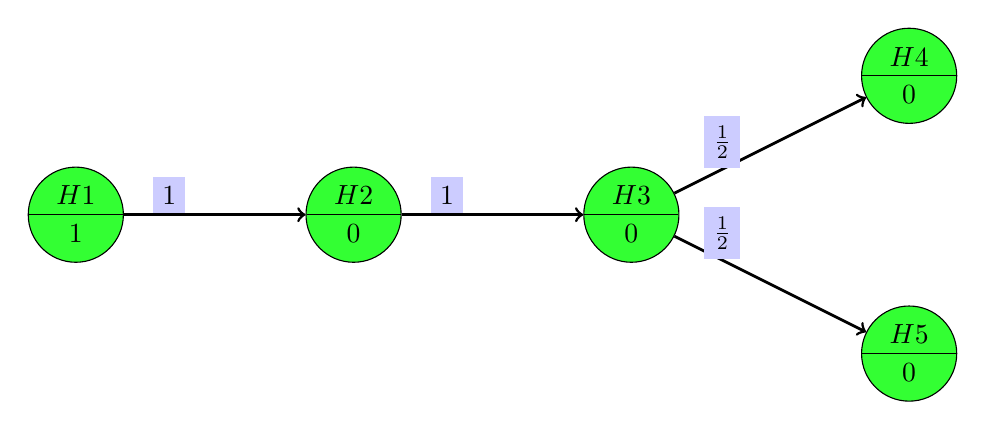
\begin{tikzpicture}

\node (H1) at (125bp,-125bp)[draw,circle split,fill=green!80] {$H1$ \nodepart{lower} $1$};
\node (H2) at (225bp,-125bp)[draw,circle split,fill=green!80] {$H2$ \nodepart{lower} $0$};
\node (H3) at (325bp,-125bp)[draw,circle split,fill=green!80] {$H3$ \nodepart{lower} $0$};
\node (H4) at (425bp,-75bp)[draw,circle split,fill=green!80] {$H4$ \nodepart{lower} $0$};
\node (H5) at (425bp,-175bp)[draw,circle split,fill=green!80] {$H5$ \nodepart{lower} $0$};
\draw [->,line width=1pt] (H1) to[auto] node[near start,above,fill=blue!20] {$1$} (H2);
\draw [->,line width=1pt] (H2) to[auto] node[near start,above,fill=blue!20] {$1$} (H3);
\draw [->,line width=1pt] (H3) to[auto] node[near start,above,fill=blue!20] {$\frac{1}{2}$} (H4);
\draw [->,line width=1pt] (H3) to[auto] node[near start,above,fill=blue!20] {$\frac{1}{2}$} (H5);
\end{tikzpicture}

}
\end{center}

\end{figure}\begin{figure}[ht]
\begin{center}
\scalebox{0.7}{
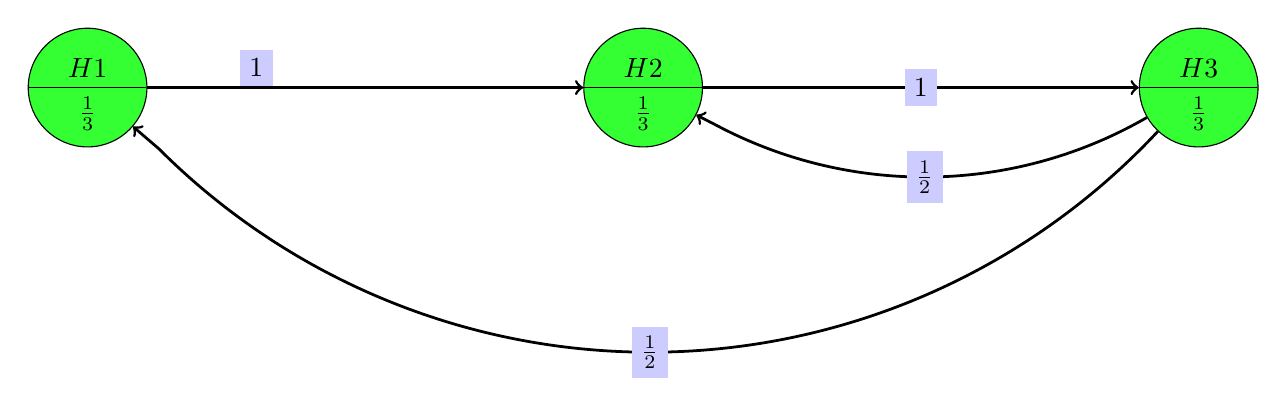
\begin{tikzpicture}

\node (H1) at (125bp,-125bp)[draw,circle split,fill=green!80] {$H1$ \nodepart{lower} $\frac{1}{3}$};
\node (H2) at (325bp,-125bp)[draw,circle split,fill=green!80] {$H2$ \nodepart{lower} $\frac{1}{3}$};
\node (H3) at (525bp,-125bp)[draw,circle split,fill=green!80] {$H3$ \nodepart{lower} $\frac{1}{3}$};
\draw [->,line width=1pt] (H1) to[auto] node[near start,above,fill=blue!20] {$1$} (H2);
\draw [->,line width=1pt] (H2) to (425bp, -125bp) node[fill=blue!20] {$1$} to (H3);
\draw [->,line width=1pt] (H3.227) arc(317:270:250bp) node[fill=blue!20] {$\frac{1}{2}$} arc(270:225:250bp) to (H1);
\draw [->,line width=1pt] (H3.210) arc(300:270:160bp) node[fill=blue!20] {$\frac{1}{2}$} arc(270:242:160bp) to (H2);
\end{tikzpicture}

}
\end{center}

\end{figure}\begin{figure}[ht]
\begin{center}
\scalebox{0.7}{
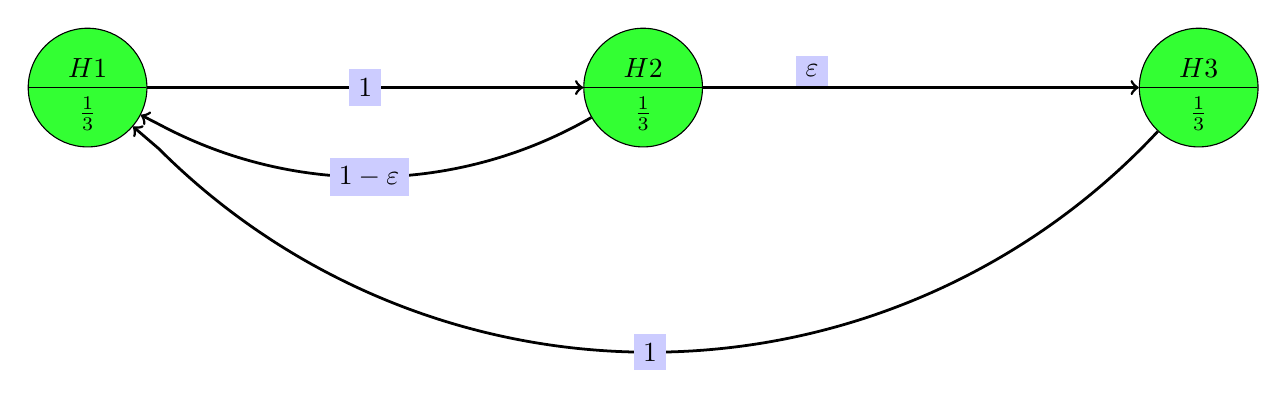
\begin{tikzpicture}

\node (H1) at (125bp,-125bp)[draw,circle split,fill=green!80] {$H1$ \nodepart{lower} $\frac{1}{3}$};
\node (H2) at (325bp,-125bp)[draw,circle split,fill=green!80] {$H2$ \nodepart{lower} $\frac{1}{3}$};
\node (H3) at (525bp,-125bp)[draw,circle split,fill=green!80] {$H3$ \nodepart{lower} $\frac{1}{3}$};
\draw [->,line width=1pt] (H1) to (225bp, -125bp) node[fill=blue!20] {$1$} to (H2);
\draw [->,line width=1pt] (H2.210) arc(300:270:160bp) node[fill=blue!20] {$1-\epsilon$} arc(270:242:160bp) to (H1);
\draw [->,line width=1pt] (H2) to[auto] node[near start,above,fill=blue!20] {$\epsilon$} (H3);
\draw [->,line width=1pt] (H3.227) arc(317:270:250bp) node[fill=blue!20] {$1$} arc(270:225:250bp) to (H1);
\end{tikzpicture}

}
\end{center}

\end{figure}\begin{figure}[ht]
\begin{center}
\scalebox{0.7}{
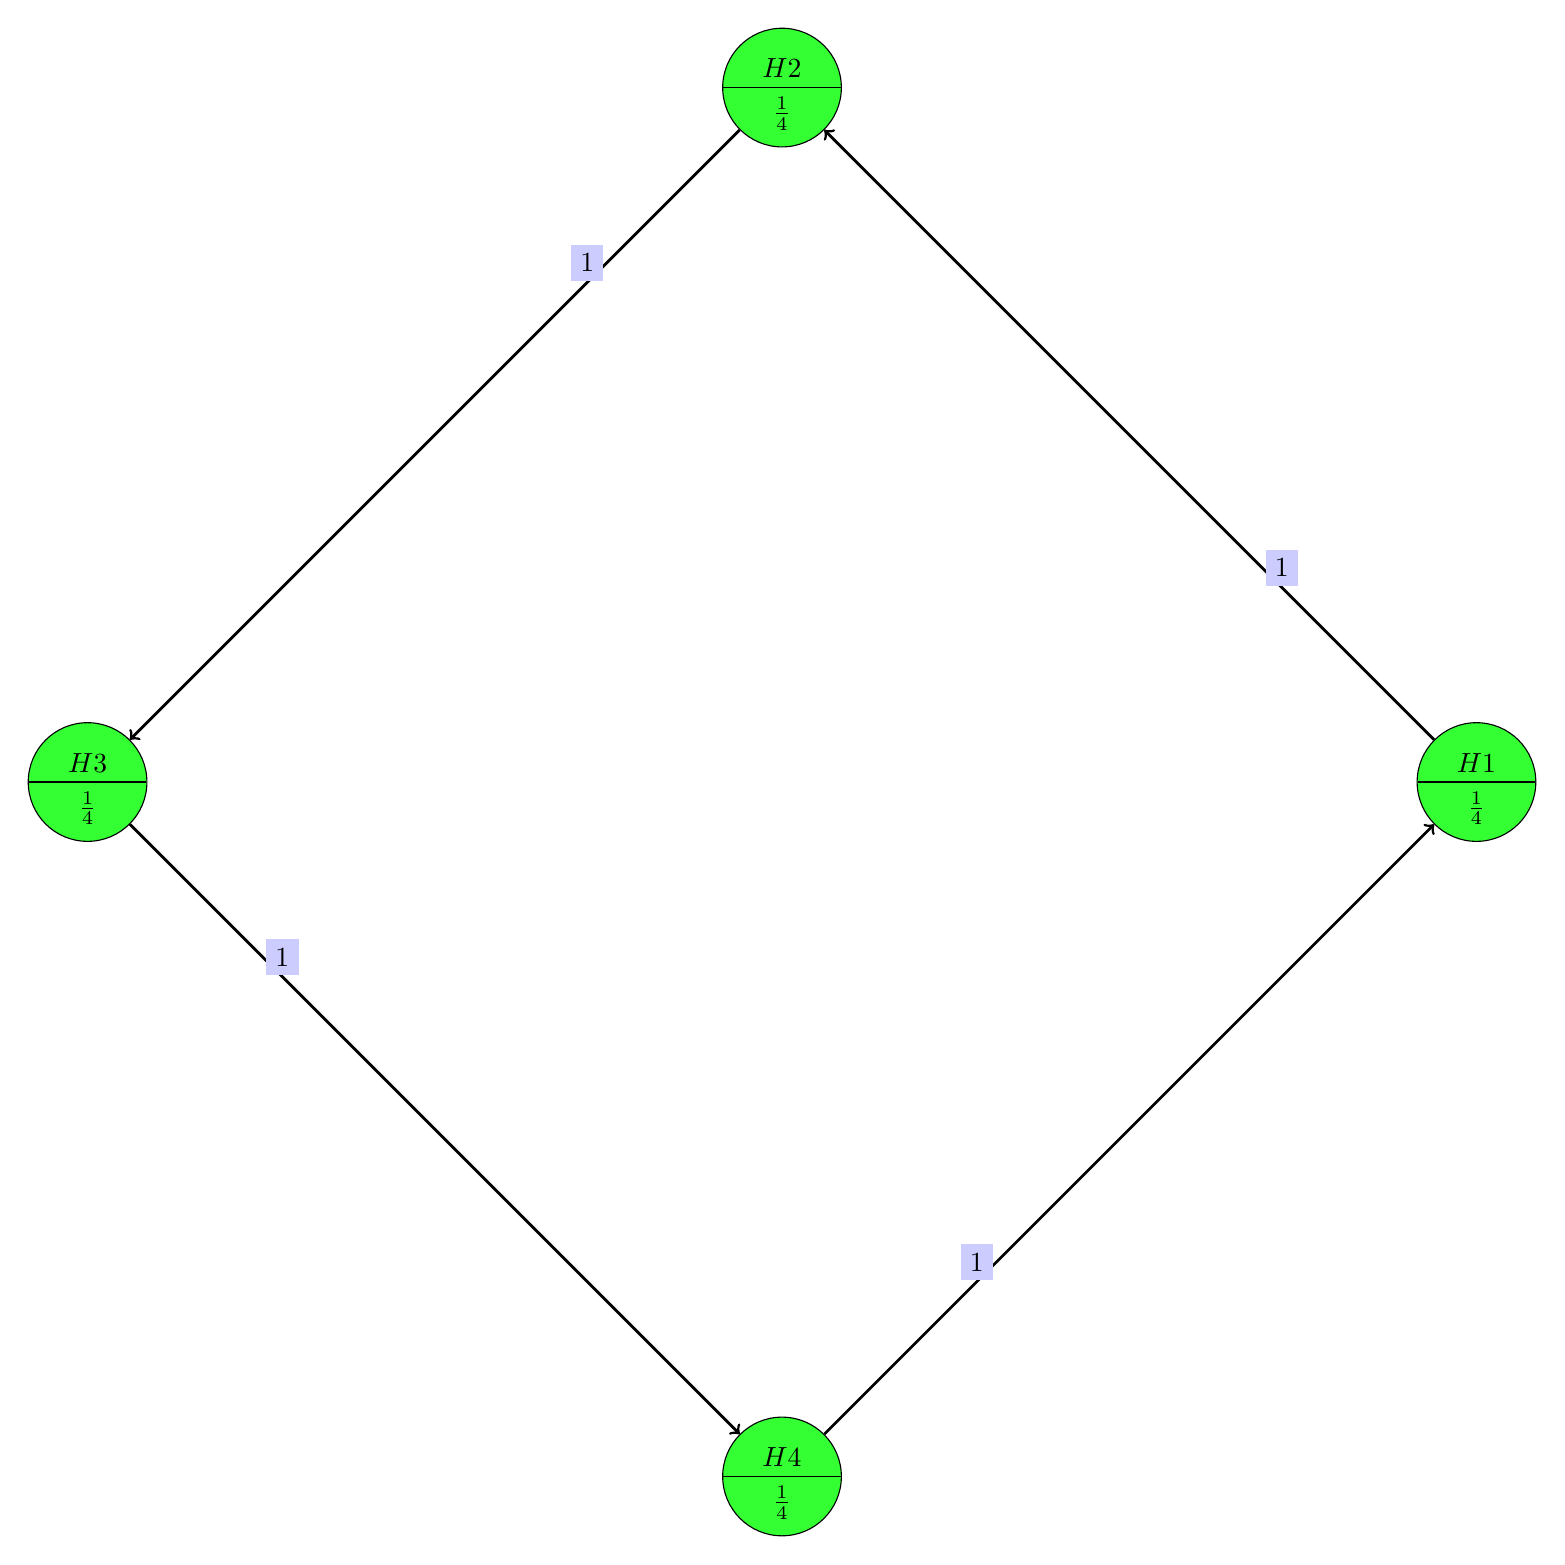
\begin{tikzpicture}

\node (H1) at (575bp,-325bp)[draw,circle split,fill=green!80] {$H1$ \nodepart{lower} $\frac{1}{4}$};
\node (H2) at (325bp,-75bp)[draw,circle split,fill=green!80] {$H2$ \nodepart{lower} $\frac{1}{4}$};
\node (H3) at (75bp,-325bp)[draw,circle split,fill=green!80] {$H3$ \nodepart{lower} $\frac{1}{4}$};
\node (H4) at (325bp,-575bp)[draw,circle split,fill=green!80] {$H4$ \nodepart{lower} $\frac{1}{4}$};
\draw [->,line width=1pt] (H1) to[auto] node[near start,above,fill=blue!20] {$1$} (H2);
\draw [->,line width=1pt] (H2) to[auto] node[near start,above,fill=blue!20] {$1$} (H3);
\draw [->,line width=1pt] (H3) to[auto] node[near start,above,fill=blue!20] {$1$} (H4);
\draw [->,line width=1pt] (H4) to[auto] node[near start,above,fill=blue!20] {$1$} (H1);
\end{tikzpicture}

}
\end{center}

\end{figure}\begin{figure}[ht]
\begin{center}
\scalebox{0.7}{
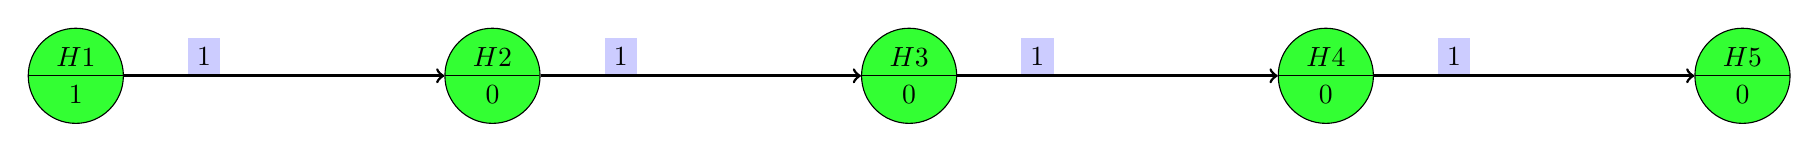
\begin{tikzpicture}

\node (H1) at (75bp,-125bp)[draw,circle split,fill=green!80] {$H1$ \nodepart{lower} $1$};
\node (H2) at (225bp,-125bp)[draw,circle split,fill=green!80] {$H2$ \nodepart{lower} $0$};
\node (H3) at (375bp,-125bp)[draw,circle split,fill=green!80] {$H3$ \nodepart{lower} $0$};
\node (H4) at (525bp,-125bp)[draw,circle split,fill=green!80] {$H4$ \nodepart{lower} $0$};
\node (H5) at (675bp,-125bp)[draw,circle split,fill=green!80] {$H5$ \nodepart{lower} $0$};
\draw [->,line width=1pt] (H1) to[auto] node[near start,above,fill=blue!20] {$1$} (H2);
\draw [->,line width=1pt] (H2) to[auto] node[near start,above,fill=blue!20] {$1$} (H3);
\draw [->,line width=1pt] (H3) to[auto] node[near start,above,fill=blue!20] {$1$} (H4);
\draw [->,line width=1pt] (H4) to[auto] node[near start,above,fill=blue!20] {$1$} (H5);
\end{tikzpicture}

}
\end{center}

\end{figure}\begin{figure}[ht]
\begin{center}
\scalebox{0.7}{
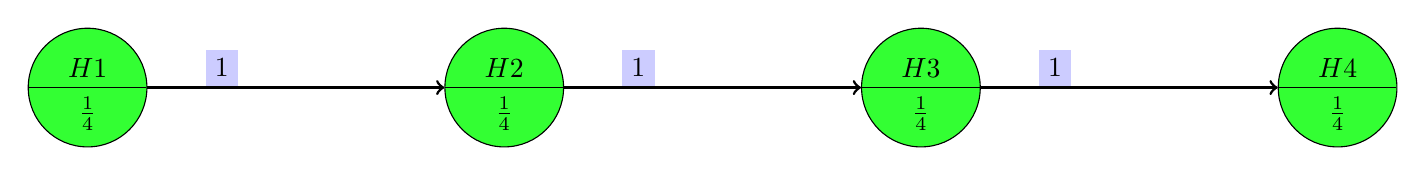
\begin{tikzpicture}

\node (H1) at (75bp,-125bp)[draw,circle split,fill=green!80] {$H1$ \nodepart{lower} $\frac{1}{4}$};
\node (H2) at (225bp,-125bp)[draw,circle split,fill=green!80] {$H2$ \nodepart{lower} $\frac{1}{4}$};
\node (H3) at (375bp,-125bp)[draw,circle split,fill=green!80] {$H3$ \nodepart{lower} $\frac{1}{4}$};
\node (H4) at (525bp,-125bp)[draw,circle split,fill=green!80] {$H4$ \nodepart{lower} $\frac{1}{4}$};
\draw [->,line width=1pt] (H1) to[auto] node[near start,above,fill=blue!20] {$1$} (H2);
\draw [->,line width=1pt] (H2) to[auto] node[near start,above,fill=blue!20] {$1$} (H3);
\draw [->,line width=1pt] (H3) to[auto] node[near start,above,fill=blue!20] {$1$} (H4);
\end{tikzpicture}

}
\end{center}

\end{figure}\cleardoublepage
\begin{figure}[ht]
\begin{center}
\scalebox{0.7}{
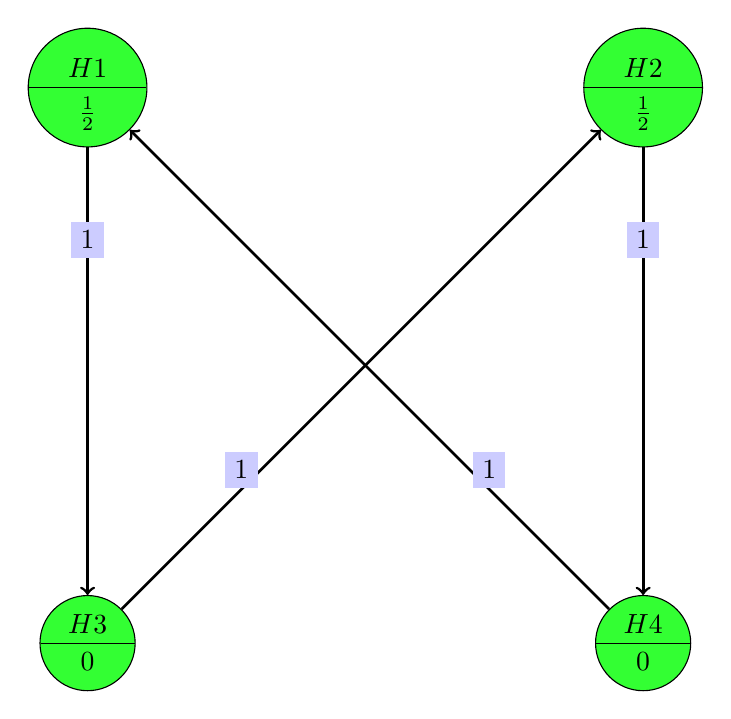
\begin{tikzpicture}

\node (H1) at (125bp,-125bp)[draw,circle split,fill=green!80] {$H1$ \nodepart{lower} $\frac{1}{2}$};
\node (H2) at (325bp,-125bp)[draw,circle split,fill=green!80] {$H2$ \nodepart{lower} $\frac{1}{2}$};
\node (H3) at (125bp,-325bp)[draw,circle split,fill=green!80] {$H3$ \nodepart{lower} $0$};
\node (H4) at (325bp,-325bp)[draw,circle split,fill=green!80] {$H4$ \nodepart{lower} $0$};
\draw [->,line width=1pt] (H1) to[auto] node[near start,above,fill=blue!20] {$1$} (H3);
\draw [->,line width=1pt] (H2) to[auto] node[near start,above,fill=blue!20] {$1$} (H4);
\draw [->,line width=1pt] (H3) to[auto] node[near start,above,fill=blue!20] {$1$} (H2);
\draw [->,line width=1pt] (H4) to[auto] node[near start,above,fill=blue!20] {$1$} (H1);
\end{tikzpicture}

}
\end{center}

\end{figure}\begin{figure}[ht]
\begin{center}
\scalebox{0.7}{
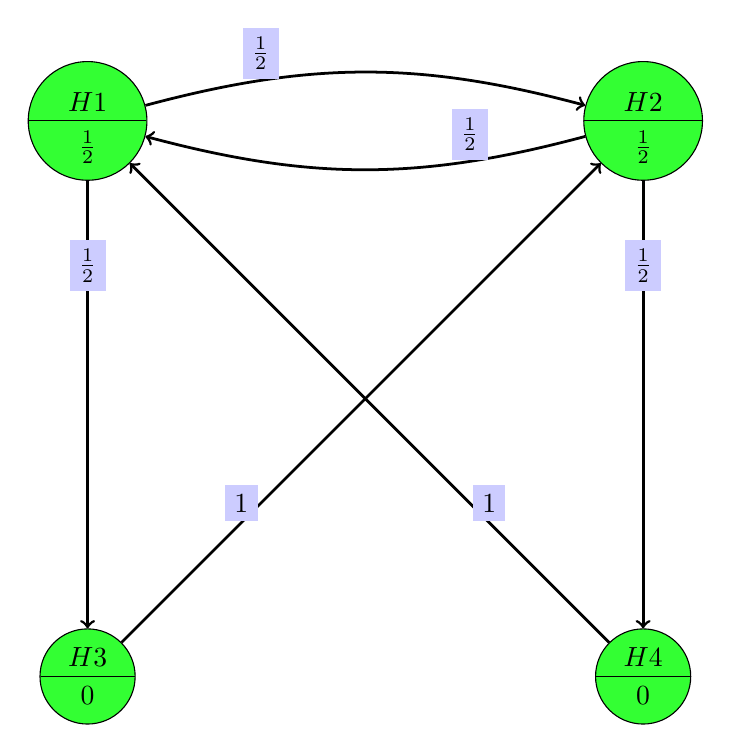
\begin{tikzpicture}

\node (H1) at (125bp,-125bp)[draw,circle split,fill=green!80] {$H1$ \nodepart{lower} $\frac{1}{2}$};
\node (H2) at (325bp,-125bp)[draw,circle split,fill=green!80] {$H2$ \nodepart{lower} $\frac{1}{2}$};
\node (H3) at (125bp,-325bp)[draw,circle split,fill=green!80] {$H3$ \nodepart{lower} $0$};
\node (H4) at (325bp,-325bp)[draw,circle split,fill=green!80] {$H4$ \nodepart{lower} $0$};
\draw [->,line width=1pt] (H1) to[bend left=15] node[near start,above,fill=blue!20] {$\frac{1}{2}$} (H2);
\draw [->,line width=1pt] (H1) to[auto] node[near start,above,fill=blue!20] {$\frac{1}{2}$} (H3);
\draw [->,line width=1pt] (H2) to[bend left=15] node[near start,above,fill=blue!20] {$\frac{1}{2}$} (H1);
\draw [->,line width=1pt] (H2) to[auto] node[near start,above,fill=blue!20] {$\frac{1}{2}$} (H4);
\draw [->,line width=1pt] (H3) to[auto] node[near start,above,fill=blue!20] {$1$} (H2);
\draw [->,line width=1pt] (H4) to[auto] node[near start,above,fill=blue!20] {$1$} (H1);
\end{tikzpicture}

}
\end{center}

\end{figure}\begin{figure}[ht]
\begin{center}
\scalebox{0.7}{
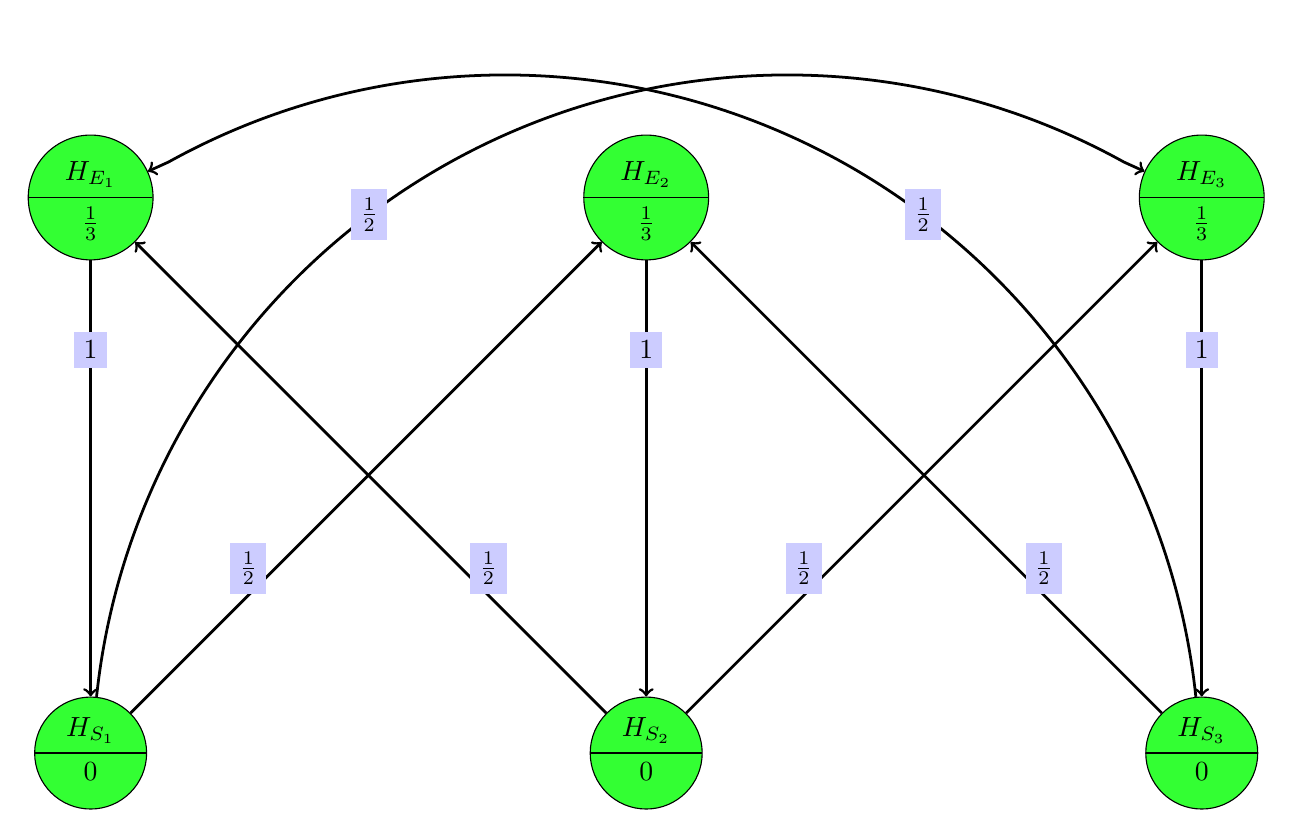
\begin{tikzpicture}

\node (HE1) at (125bp,-125bp)[draw,circle split,fill=green!80] {$H_{E_1}$ \nodepart{lower} $\frac{1}{3}$};
\node (HE2) at (325bp,-125bp)[draw,circle split,fill=green!80] {$H_{E_2}$ \nodepart{lower} $\frac{1}{3}$};
\node (HE3) at (525bp,-125bp)[draw,circle split,fill=green!80] {$H_{E_3}$ \nodepart{lower} $\frac{1}{3}$};
\node (HS1) at (125bp,-325bp)[draw,circle split,fill=green!80] {$H_{S_1}$ \nodepart{lower} $0$};
\node (HS2) at (325bp,-325bp)[draw,circle split,fill=green!80] {$H_{S_2}$ \nodepart{lower} $0$};
\node (HS3) at (525bp,-325bp)[draw,circle split,fill=green!80] {$H_{S_3}$ \nodepart{lower} $0$};
\draw [->,line width=1pt] (HE1) to[auto] node[near start,above,fill=blue!20] {$1$} (HS1);
\draw [->,line width=1pt] (HE2) to[auto] node[near start,above,fill=blue!20] {$1$} (HS2);
\draw [->,line width=1pt] (HE3) to[auto] node[near start,above,fill=blue!20] {$1$} (HS3);
\draw [->,line width=1pt] (HS1) to[auto] node[near start,above,fill=blue!20] {$\frac{1}{2}$} (HE2);
\draw [->,line width=1pt] (HS1.84) arc(174:127:250bp) node[fill=blue!20] {$\frac{1}{2}$} arc(127:61:250bp) to (HE3);
\draw [->,line width=1pt] (HS2) to[auto] node[near start,above,fill=blue!20] {$\frac{1}{2}$} (HE1);
\draw [->,line width=1pt] (HS2) to[auto] node[near start,above,fill=blue!20] {$\frac{1}{2}$} (HE3);
\draw [->,line width=1pt] (HS3.96) arc(6:53:250bp) node[fill=blue!20] {$\frac{1}{2}$} arc(53:119:250bp) to (HE1);
\draw [->,line width=1pt] (HS3) to[auto] node[near start,above,fill=blue!20] {$\frac{1}{2}$} (HE2);
\end{tikzpicture}

}
\end{center}

\end{figure}\begin{figure}[ht]
\begin{center}
\scalebox{0.7}{
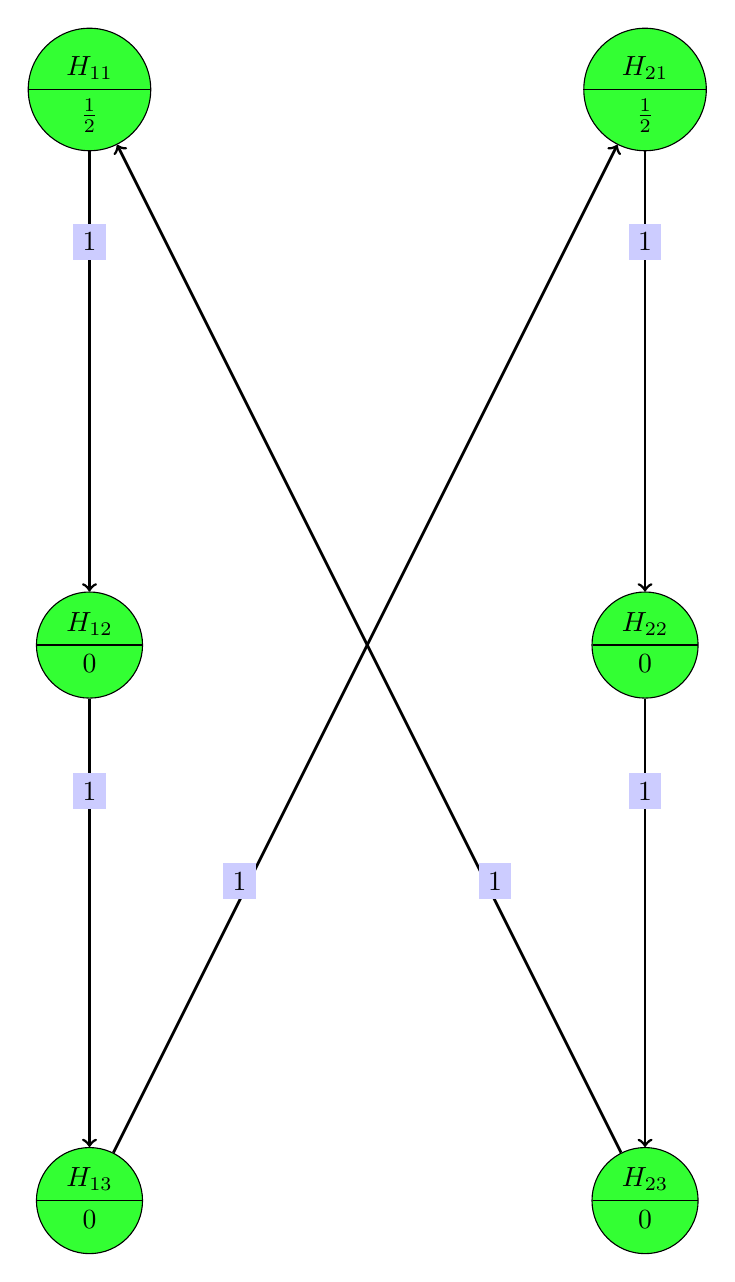
\begin{tikzpicture}

\node (H11) at (125bp,-125bp)[draw,circle split,fill=green!80] {$H_{11}$ \nodepart{lower} $\frac{1}{2}$};
\node (H21) at (325bp,-125bp)[draw,circle split,fill=green!80] {$H_{21}$ \nodepart{lower} $\frac{1}{2}$};
\node (H12) at (125bp,-325bp)[draw,circle split,fill=green!80] {$H_{12}$ \nodepart{lower} $0$};
\node (H22) at (325bp,-325bp)[draw,circle split,fill=green!80] {$H_{22}$ \nodepart{lower} $0$};
\node (H13) at (125bp,-525bp)[draw,circle split,fill=green!80] {$H_{13}$ \nodepart{lower} $0$};
\node (H23) at (325bp,-525bp)[draw,circle split,fill=green!80] {$H_{23}$ \nodepart{lower} $0$};
\draw [->,line width=1pt] (H11) to[auto] node[near start,above,fill=blue!20] {$1$} (H12);
\draw [->,line width=1pt] (H21) to[auto] node[near start,above,fill=blue!20] {$1$} (H22);
\draw [->,line width=1pt] (H12) to[auto] node[near start,above,fill=blue!20] {$1$} (H13);
\draw [->,line width=1pt] (H22) to[auto] node[near start,above,fill=blue!20] {$1$} (H23);
\draw [->,line width=1pt] (H13) to[auto] node[near start,above,fill=blue!20] {$1$} (H21);
\draw [->,line width=1pt] (H23) to[auto] node[near start,above,fill=blue!20] {$1$} (H11);
\end{tikzpicture}

}
\end{center}

\end{figure}\begin{figure}[ht]
\begin{center}
\scalebox{0.7}{
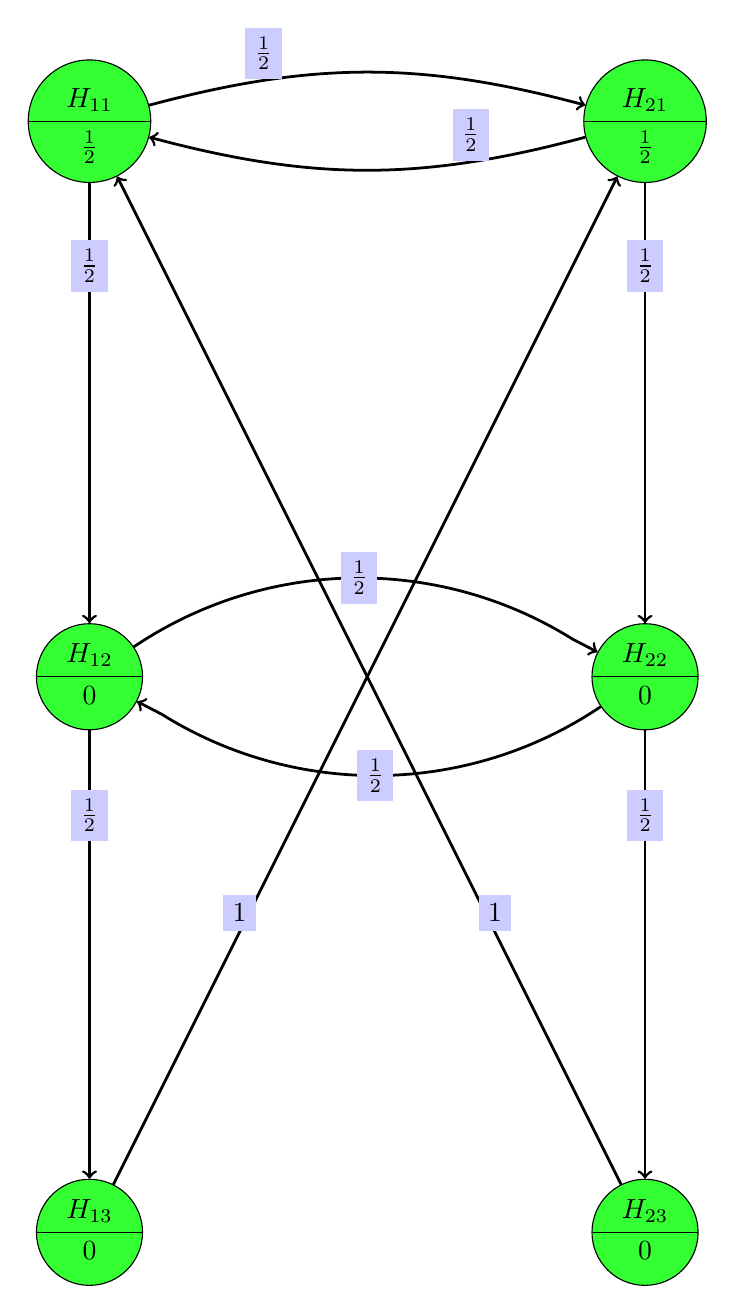
\begin{tikzpicture}

\node (H11) at (125bp,-125bp)[draw,circle split,fill=green!80] {$H_{11}$ \nodepart{lower} $\frac{1}{2}$};
\node (H21) at (325bp,-125bp)[draw,circle split,fill=green!80] {$H_{21}$ \nodepart{lower} $\frac{1}{2}$};
\node (H12) at (125bp,-325bp)[draw,circle split,fill=green!80] {$H_{12}$ \nodepart{lower} $0$};
\node (H22) at (325bp,-325bp)[draw,circle split,fill=green!80] {$H_{22}$ \nodepart{lower} $0$};
\node (H13) at (125bp,-525bp)[draw,circle split,fill=green!80] {$H_{13}$ \nodepart{lower} $0$};
\node (H23) at (325bp,-525bp)[draw,circle split,fill=green!80] {$H_{23}$ \nodepart{lower} $0$};
\draw [->,line width=1pt] (H11) to[bend left=15] node[near start,above,fill=blue!20] {$\frac{1}{2}$} (H21);
\draw [->,line width=1pt] (H11) to[auto] node[near start,above,fill=blue!20] {$\frac{1}{2}$} (H12);
\draw [->,line width=1pt] (H21) to[bend left=15] node[near start,above,fill=blue!20] {$\frac{1}{2}$} (H11);
\draw [->,line width=1pt] (H21) to[auto] node[near start,above,fill=blue!20] {$\frac{1}{2}$} (H22);
\draw [->,line width=1pt] (H12.34) arc(124:90:145bp) node[fill=blue!20] {$\frac{1}{2}$} arc(90:58:145bp) to (H22);
\draw [->,line width=1pt] (H12) to[auto] node[near start,above,fill=blue!20] {$\frac{1}{2}$} (H13);
\draw [->,line width=1pt] (H22.214) arc(304:270:145bp) node[fill=blue!20] {$\frac{1}{2}$} arc(270:238:145bp) to (H12);
\draw [->,line width=1pt] (H22) to[auto] node[near start,above,fill=blue!20] {$\frac{1}{2}$} (H23);
\draw [->,line width=1pt] (H13) to[auto] node[near start,above,fill=blue!20] {$1$} (H21);
\draw [->,line width=1pt] (H23) to[auto] node[near start,above,fill=blue!20] {$1$} (H11);
\end{tikzpicture}

}
\end{center}

\end{figure}\begin{figure}[ht]
\begin{center}
\scalebox{0.7}{
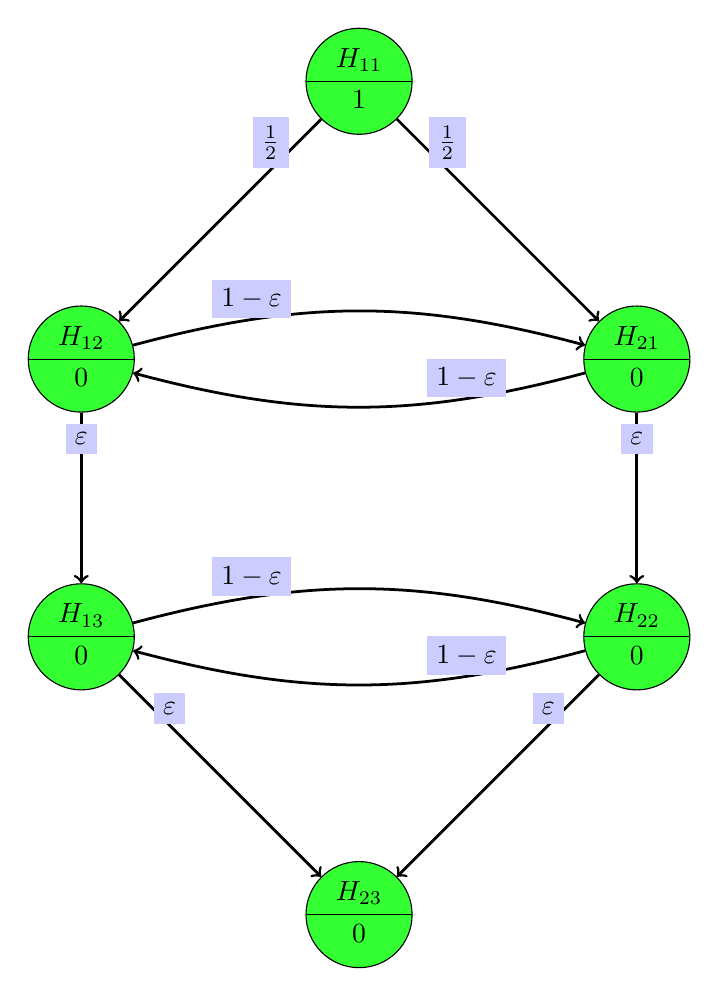
\begin{tikzpicture}

\node (H11) at (225bp,-125bp)[draw,circle split,fill=green!80] {$H_{11}$ \nodepart{lower} $1$};
\node (H21) at (325bp,-225bp)[draw,circle split,fill=green!80] {$H_{21}$ \nodepart{lower} $0$};
\node (H12) at (125bp,-225bp)[draw,circle split,fill=green!80] {$H_{12}$ \nodepart{lower} $0$};
\node (H22) at (325bp,-325bp)[draw,circle split,fill=green!80] {$H_{22}$ \nodepart{lower} $0$};
\node (H13) at (125bp,-325bp)[draw,circle split,fill=green!80] {$H_{13}$ \nodepart{lower} $0$};
\node (H23) at (225bp,-425bp)[draw,circle split,fill=green!80] {$H_{23}$ \nodepart{lower} $0$};
\draw [->,line width=1pt] (H11) to[auto] node[near start,above,fill=blue!20] {$\frac{1}{2}$} (H21);
\draw [->,line width=1pt] (H11) to[auto] node[near start,above,fill=blue!20] {$\frac{1}{2}$} (H12);
\draw [->,line width=1pt] (H21) to[bend left=15] node[near start,above,fill=blue!20] {$1-\epsilon$} (H12);
\draw [->,line width=1pt] (H21) to[auto] node[near start,above,fill=blue!20] {$\epsilon$} (H22);
\draw [->,line width=1pt] (H12) to[bend left=15] node[near start,above,fill=blue!20] {$1-\epsilon$} (H21);
\draw [->,line width=1pt] (H12) to[auto] node[near start,above,fill=blue!20] {$\epsilon$} (H13);
\draw [->,line width=1pt] (H22) to[bend left=15] node[near start,above,fill=blue!20] {$1-\epsilon$} (H13);
\draw [->,line width=1pt] (H22) to[auto] node[near start,above,fill=blue!20] {$\epsilon$} (H23);
\draw [->,line width=1pt] (H13) to[bend left=15] node[near start,above,fill=blue!20] {$1-\epsilon$} (H22);
\draw [->,line width=1pt] (H13) to[auto] node[near start,above,fill=blue!20] {$\epsilon$} (H23);
\end{tikzpicture}

}
\end{center}

\end{figure}\cleardoublepage
\begin{figure}[ht]
\begin{center}
\scalebox{0.7}{
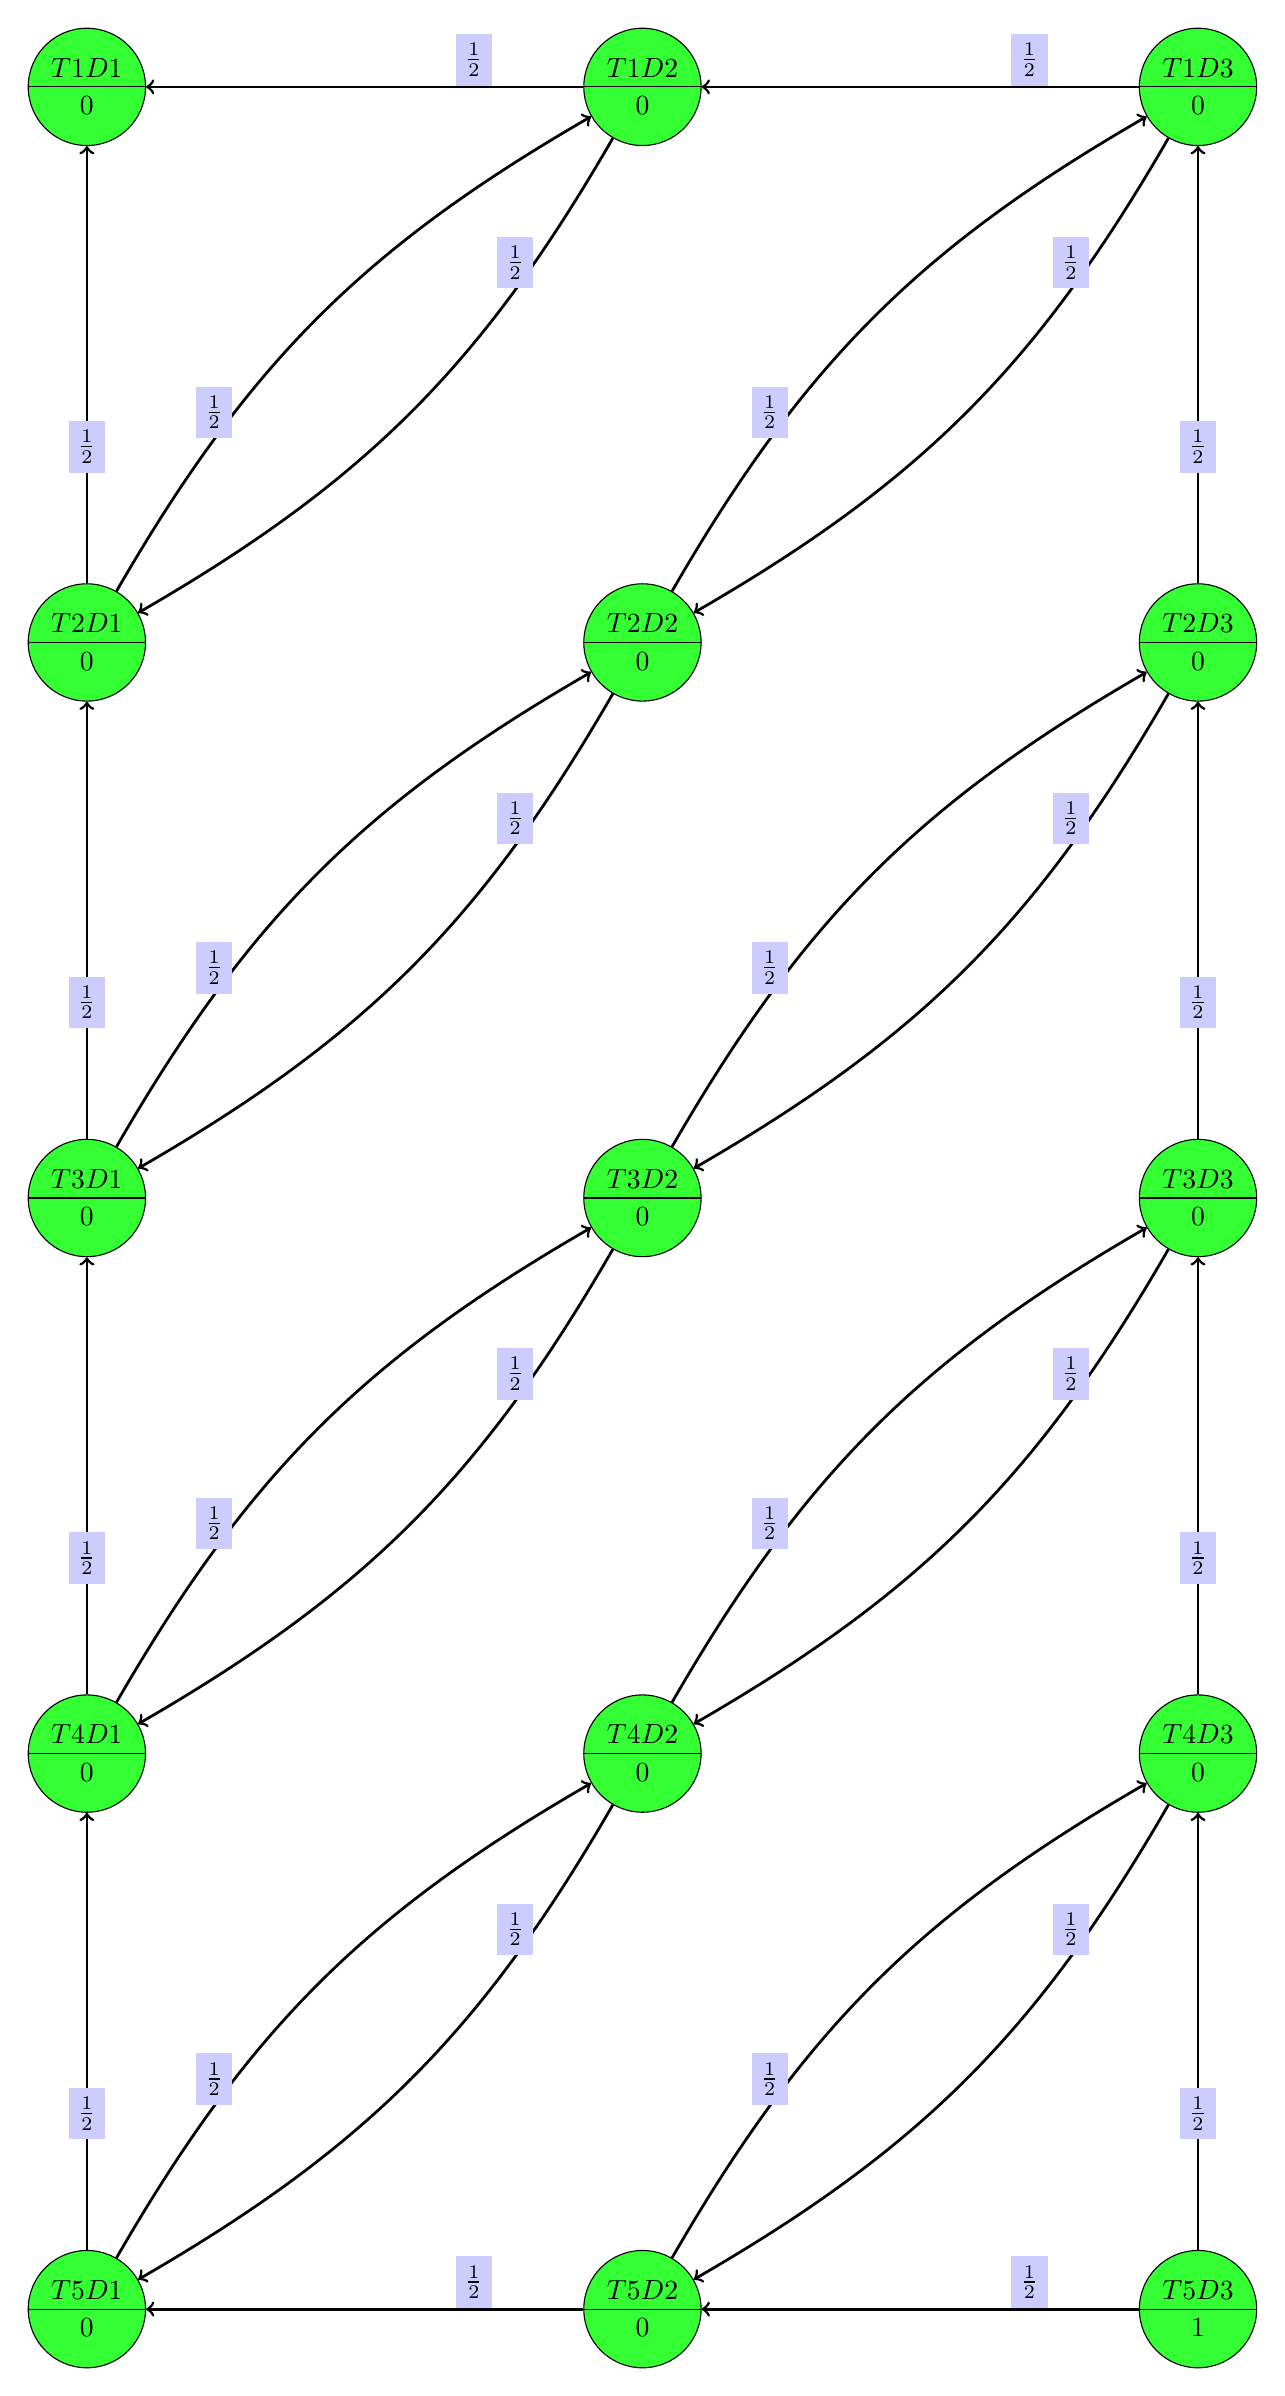
\begin{tikzpicture}

\node (T1D1) at (125bp,-125bp)[draw,circle split,fill=green!80] {$T1D1$ \nodepart{lower} $0$};
\node (T1D2) at (325bp,-125bp)[draw,circle split,fill=green!80] {$T1D2$ \nodepart{lower} $0$};
\node (T1D3) at (525bp,-125bp)[draw,circle split,fill=green!80] {$T1D3$ \nodepart{lower} $0$};
\node (T2D1) at (125bp,-325bp)[draw,circle split,fill=green!80] {$T2D1$ \nodepart{lower} $0$};
\node (T2D2) at (325bp,-325bp)[draw,circle split,fill=green!80] {$T2D2$ \nodepart{lower} $0$};
\node (T2D3) at (525bp,-325bp)[draw,circle split,fill=green!80] {$T2D3$ \nodepart{lower} $0$};
\node (T3D1) at (125bp,-525bp)[draw,circle split,fill=green!80] {$T3D1$ \nodepart{lower} $0$};
\node (T3D2) at (325bp,-525bp)[draw,circle split,fill=green!80] {$T3D2$ \nodepart{lower} $0$};
\node (T3D3) at (525bp,-525bp)[draw,circle split,fill=green!80] {$T3D3$ \nodepart{lower} $0$};
\node (T4D1) at (125bp,-725bp)[draw,circle split,fill=green!80] {$T4D1$ \nodepart{lower} $0$};
\node (T4D2) at (325bp,-725bp)[draw,circle split,fill=green!80] {$T4D2$ \nodepart{lower} $0$};
\node (T4D3) at (525bp,-725bp)[draw,circle split,fill=green!80] {$T4D3$ \nodepart{lower} $0$};
\node (T5D1) at (125bp,-925bp)[draw,circle split,fill=green!80] {$T5D1$ \nodepart{lower} $0$};
\node (T5D2) at (325bp,-925bp)[draw,circle split,fill=green!80] {$T5D2$ \nodepart{lower} $0$};
\node (T5D3) at (525bp,-925bp)[draw,circle split,fill=green!80] {$T5D3$ \nodepart{lower} $1$};
\draw [->,line width=1pt] (T1D2) to[auto] node[near start,above,fill=blue!20] {$\frac{1}{2}$} (T1D1);
\draw [->,line width=1pt] (T1D2) to[bend left=15] node[near start,above,fill=blue!20] {$\frac{1}{2}$} (T2D1);
\draw [->,line width=1pt] (T1D3) to[auto] node[near start,above,fill=blue!20] {$\frac{1}{2}$} (T1D2);
\draw [->,line width=1pt] (T1D3) to[bend left=15] node[near start,above,fill=blue!20] {$\frac{1}{2}$} (T2D2);
\draw [->,line width=1pt] (T2D1) to[auto] node[near start,above,fill=blue!20] {$\frac{1}{2}$} (T1D1);
\draw [->,line width=1pt] (T2D1) to[bend left=15] node[near start,above,fill=blue!20] {$\frac{1}{2}$} (T1D2);
\draw [->,line width=1pt] (T2D2) to[bend left=15] node[near start,above,fill=blue!20] {$\frac{1}{2}$} (T1D3);
\draw [->,line width=1pt] (T2D2) to[bend left=15] node[near start,above,fill=blue!20] {$\frac{1}{2}$} (T3D1);
\draw [->,line width=1pt] (T2D3) to[auto] node[near start,above,fill=blue!20] {$\frac{1}{2}$} (T1D3);
\draw [->,line width=1pt] (T2D3) to[bend left=15] node[near start,above,fill=blue!20] {$\frac{1}{2}$} (T3D2);
\draw [->,line width=1pt] (T3D1) to[auto] node[near start,above,fill=blue!20] {$\frac{1}{2}$} (T2D1);
\draw [->,line width=1pt] (T3D1) to[bend left=15] node[near start,above,fill=blue!20] {$\frac{1}{2}$} (T2D2);
\draw [->,line width=1pt] (T3D2) to[bend left=15] node[near start,above,fill=blue!20] {$\frac{1}{2}$} (T2D3);
\draw [->,line width=1pt] (T3D2) to[bend left=15] node[near start,above,fill=blue!20] {$\frac{1}{2}$} (T4D1);
\draw [->,line width=1pt] (T3D3) to[auto] node[near start,above,fill=blue!20] {$\frac{1}{2}$} (T2D3);
\draw [->,line width=1pt] (T3D3) to[bend left=15] node[near start,above,fill=blue!20] {$\frac{1}{2}$} (T4D2);
\draw [->,line width=1pt] (T4D1) to[auto] node[near start,above,fill=blue!20] {$\frac{1}{2}$} (T3D1);
\draw [->,line width=1pt] (T4D1) to[bend left=15] node[near start,above,fill=blue!20] {$\frac{1}{2}$} (T3D2);
\draw [->,line width=1pt] (T4D2) to[bend left=15] node[near start,above,fill=blue!20] {$\frac{1}{2}$} (T3D3);
\draw [->,line width=1pt] (T4D2) to[bend left=15] node[near start,above,fill=blue!20] {$\frac{1}{2}$} (T5D1);
\draw [->,line width=1pt] (T4D3) to[auto] node[near start,above,fill=blue!20] {$\frac{1}{2}$} (T3D3);
\draw [->,line width=1pt] (T4D3) to[bend left=15] node[near start,above,fill=blue!20] {$\frac{1}{2}$} (T5D2);
\draw [->,line width=1pt] (T5D1) to[auto] node[near start,above,fill=blue!20] {$\frac{1}{2}$} (T4D1);
\draw [->,line width=1pt] (T5D1) to[bend left=15] node[near start,above,fill=blue!20] {$\frac{1}{2}$} (T4D2);
\draw [->,line width=1pt] (T5D2) to[bend left=15] node[near start,above,fill=blue!20] {$\frac{1}{2}$} (T4D3);
\draw [->,line width=1pt] (T5D2) to[auto] node[near start,above,fill=blue!20] {$\frac{1}{2}$} (T5D1);
\draw [->,line width=1pt] (T5D3) to[auto] node[near start,above,fill=blue!20] {$\frac{1}{2}$} (T4D3);
\draw [->,line width=1pt] (T5D3) to[auto] node[near start,above,fill=blue!20] {$\frac{1}{2}$} (T5D2);
\end{tikzpicture}

}
\end{center}

\end{figure}


\cleardoublepage

\section{Appendix - Multiple Testing Basics}

Let $\Theta$ be a parameter space indexing a family of probabilities
$\{P_\theta\;|\;\theta\in\Theta\}$ and $(\Omega, \sF, P_\theta)$ the
associated probability spaces.  For a family of null hypotheses
$H_i\subset\Theta$, $i\in\{1,\ldots,n\}=:I$ a multiple test procedure
$\phi$ is defined as a family of $(\sF, \Pot(\{0,1\}^n))$-measurable
functions $\{\phi_J:\; \Omega \rightarrow \{0,1\}^n\;|\;J\subset I\}$.
(We'll write $\phi_j$ for $\phi_\{j\}$). 

The family of hypotheses $\{H_i \;|\;i\in I\}$ is called
\emph{closed}\index{closed family} if it is closed under intersection. 

\begin{Def}[Familywise Error Rate]\index{familywise error rate}
  Let $H_J:=\bigcap_{j\in J} H_j$. The multiple test procedure $\phi$
  controls the \emph{familywise error rate at level $\alpha$ in the
    weak sense} if
  \[\forall \theta\in H_I: \; P_\theta(\phi_J=1\text{ for some }J\subset I)\leq\alpha.\]
  The multiple test procedure $\phi$ controls the \emph{familywise
    error rate at level $\alpha$ in the strong sense} if
  \[\forall \theta\in\Theta: \; P_\theta\left(\max\limits_{J\subset I, \theta\in H_J}\phi_J=1\right)\leq\alpha.\]
  %\[\forall \theta\in\Theta: \; P_\theta(\phi_J=1\text{ and }\theta\in H_J\text{ for some }J\subset I)\leq\alpha.\]
\end{Def}

This section is work in progress.

%\subsection{Closed testing principle}\index{closed testing principle}
\begin{Theorem}[Closed testing principle]\index{closed testing principle}
 \cite{marcus1976closed}
\end{Theorem}

\begin{Def}[Coherence and Consonance]
  A multiple test procedure is called \emph{consonant}\index{consonance} if 
  \[\forall J\subset I:\; \left(\phi_J=1\;\Rightarrow\;\exists j\in J:\;\phi_j=1\right).\]
  %or in other words if $\Cap_{j\in J}H_j$ can be rejected than there exists a $H_j$, $j\in J$ that is rejected. 

  A multiple test procedure is called \emph{coherent}\index{coherence} if
  \[\forall J,\,J'\subset I:\; \left(\phi_J=0\text{ and }J'\subset J\;\Rightarrow\;\phi_{J'}=0\right).\]

  For further reading see
  \cite{hochberg2009multiple} and \cite{gabriel1969simultaneous}.
\end{Def}

%\subsection{Partitioning principle}\index{partitioning principle}

\begin{Def}

\end{Def}

\begin{Theorem}[Simes-Procedure]\index{Simes-Procedure} 
Let $T_1, \ldots, T_m$
be test statistics for $m\in\N$ null hypotheses $H_1, \ldots, H_m$ and
$p_1, \ldots, p_m$ the associated p-values and $\alpha\in]0,1[$.
%Then the following test will control the familywise error rate at level $\alpha\in]0,1[$ in the strong sense:

Denote the ordered p-values by $p^{(1)}<p^{(2)}<\ldots<p^{(m)}$ 
and the corresponding hypotheses by $H^{(1)},H^{(2)},\ldots, H^{(m)}$.

Reject $H_0$ if
\[p^{(j)}\leq\frac{j\alpha}{n}\quad\text{for some $1\leq j\leq m$}.\]

For independent tests the FWER is controlled at level $\alpha$.
\end{Theorem}

\begin{Theorem}[Weighted Simes Procedure]\index{Weighted Simes Procedure} 
Benjamini and Hochberg (1997)

Let $\sum_{k=1}^m w_k = m$ and reject $H_0$ if
\[p^{(j)}\leq\frac{\sum_{k=1}^jw_[{(k)}}{m}\cdot\alpha\quad\text{for some $1\leq j\leq m$}.\]

\end{Theorem}

\begin{Theorem}[Hommel Procedure]\index{Hommel Procedure} 
Hommel 1988
\end{Theorem}

\begin{Theorem}[Hochberg Procedure]\index{Hochberg procedure}
Hochberg 1988
\end{Theorem}

Adjusted p-values form the Hochberg Procedure are greater as or equal
to the Hommel-adjusted p-values.

\subsubsection*{Adjusted p-Values in the Simes Test}

For each set $J\subset I$ we calculate
\[m_J := \min\limits_{j\in J}\left(\frac{p_j}{\sum_{i\in J_j}w_i}\right),\quad J_j=\{k\in J\;|\; p_k\leq p_j\}.\]

The weighted Simes Test rejects $H_J$ iff $m_J\leq\alpha$.
%for some $j \in J$
%\[p_j\leq\alpha \sum_{i\in J_j}w_i\]
%or equivalent
%\[\]

In a closed testing procedure a hypothesis $H_j$ is rejected iff $H_J$
is rejected for each $J\subset I$ with $j\in J$.

An adjusted p-pvalue $p'_j$ is defined as the minimal $\alpha$ so that
the test to global level $\alpha$ rejects $H_j$.

Therefore $p'_j=\text{max}(m_J\;|\;j\in J)$.

\section{Appendix - Graph Theory Basics}

When we talk about graphs in the context of gMCP we always mean finite,
directed, weighted graphs with no self-loops and no parallel edges:

\begin{Def}
 In our context a (valid) \emph{graph} $G$ is a triple $G=(V,E,w)$
 of a non-empty, finite set $V$ of nodes together with the set of edges
 $E\subset (V\times V)\setminus\{(v,v)\;|\;v\in V\}$ and a mapping $w:\;V\cup
 E\rightarrow [0,1]$ that fullfills $\sum_{v\in V}w(v)\leq1$ and $w(e)>0$ for
 each edge $e\in E$.
\end{Def}

Isomorphisms.

This section is work in progress.

%\begin{Theorem}[Unimprovable graph] 
% Let $G=(V,E,w)$ be a graph with $\sum_{v\in V}w(v)=1$.
% If for all $v, v'\in V$, $v\neq v'$ with $w(v)>0$ a path from $v$ to $v'$
% exists, than there is no other graph with an uniformly better
% associated test statistic.
%\begin{Proof}
%\end{Proof}
%\end{Theorem}

\end{appendix}

\newpage

\addcontentsline{toc}{section}{Index}
\printindex

\newpage

\listofalgorithms
\listoffigures
\listoftables

\newpage

\addcontentsline{toc}{section}{Literatur}
\bibliography{literatur}

\addcontentsline{toc}{section}{Table of Symbols}
\section*{Table of Symbols}\footnotesize
%\twocolumn[\section{Symbolverzeichnis}]
\begin{tabularx}{\textwidth}{lX}
\multicolumn{2}{l}{\textbf{Sets}}\\
\R& set of real numbers\\
\NN& set of natural numbers (including 0)\\
$\Pot(X)$ & power set of set $X$, i.e.\ the set of all subsets of $X$\\
\\
%\multicolumn{2}{l}{\textbf{Relationen}}\\
%$X\Subset Y$& $X$ ist relativ kompakt in $Y$\\
%\end{tabularx}\\
%\begin{tabularx}{\textwidth}{lX}
\multicolumn{2}{l}{\textbf{Functions}}\\
$\skp{\cdot,\cdot}$ & standard direct product $\skp{x,y}=\sum_{j=1}^nx_j\cdot y_j$ for $x,y\in\R^n$\\
$\id_X$ & identity on $X$, i.e.\ $\id_X:\;X\rightarrow X,\;x\mapsto x$\\
%\\
%\multicolumn{2}{l}{\textbf{Andere Symbole}}\\
\end{tabularx}
%\onecolumn

\normalsize

\newpage


\end{document}
